\documentclass[aspectratio=169,12pt]{beamer}
\usepackage[utf8]{inputenc}
\usepackage[T5]{fontenc}
\usepackage[vietnamese]{babel}
\usepackage{lmodern}
\usepackage{graphicx}
\usepackage{booktabs}
\usepackage{tabularx}
\usepackage{multicol}
\usepackage{tikz}
\usepackage{xcolor}

\usetheme{Madrid}
\usefonttheme{professionalfonts}

% --- Custom Colors & Settings ---
\definecolor{UBrandBlue}{RGB}{0, 71, 155}
\definecolor{UBrandGold}{RGB}{255, 184, 28}
\setbeamercolor{palette primary}{bg=UBrandBlue,fg=white}
\setbeamercolor{palette secondary}{bg=UBrandGold,fg=black}
\setbeamercolor{palette tertiary}{bg=UBrandBlue!80!black,fg=white}
\setbeamercolor{title}{bg=UBrandBlue,fg=white}
\setbeamercolor{item}{fg=UBrandBlue}


\title[Thực hành - Chương 05]{Chuẩn bị Dữ liệu}
\subtitle{Analysis: Data Preparation}
\author[Giảng viên]{Trí tuệ Nhân tạo cho Kế toán (AI in Accounting)}
\institute[Đại học]{Khoa Kế toán - Kiểm toán}
\date{Bài giảng Thực hành 05}

\begin{document}

\begin{frame}
    \titlepage
\end{frame}

\begin{frame}{Góc nhìn Chuyên gia (Professional Insight)}
\begin{itemize}
    \item \textbf{Thực tế 80/20:} Chuẩn bị dữ liệu thường chiếm 80\% thời gian của một dự án phân tích dữ liệu, chỉ 20\% còn lại dành cho việc phân tích thực sự.
    \item \textbf{Rác vào - Rác ra (GIGO):} Dữ liệu không được chuẩn bị kỹ lưỡng sẽ dẫn đến kết quả phân tích sai lệch, bất kể mô hình học máy (Machine Learning) có phức tạp đến đâu.
    \item \textbf{Tầm quan trọng của ETL:} Quá trình Trích xuất (Extract), Chuyển đổi (Transform), và Tải (Load) là kỹ năng cốt lõi bắt buộc đối với một Kế toán viên trong kỷ nguyên số.
\end{itemize}
\end{frame}

\begin{frame}{Lộ trình Chương (Chapter Roadmap)}
\begin{itemize}
    \item \textbf{LO 5.1:} Định hình dữ liệu (Data Profiling).
    \item \textbf{LO 5.2:} Mô tả quá trình ETL.
    \item \textbf{LO 5.3:} Mẫu trích xuất dữ liệu.
    \item \textbf{LO 5.4:} Mẫu chuyển đổi cột (Column Transformation).
    \item \textbf{LO 5.5:} Mẫu chuyển đổi bảng (Table Transformation).
    \item \textbf{LO 5.6:} Mẫu chuyển đổi mô hình dữ liệu.
    \item \textbf{LO 5.7:} Mẫu tải dữ liệu.
\end{itemize}
\end{frame}

\begin{frame}{5.1 Quá trình Định hình Dữ liệu (Data Profiling)}
\begin{itemize}
    \item \textbf{Data Profiling là gì?} Là bước khảo sát đầu tiên để hiểu rõ dữ liệu trước khi xử lý. Giống như việc "khám sức khỏe tổng quát" cho dữ liệu.
    \item \textbf{Hai bước định hình chính:}
    \begin{itemize}
        \item \textit{Điều tra chất lượng (Investigate Quality):} Tìm các giá trị bị thiếu (Missing), bất thường (Anomalies), hoặc sai định dạng.
        \item \textit{Điều tra cấu trúc (Investigate Structure):} Hiểu cách các cột (trường) và hàng (bản ghi) được tổ chức.
    \end{itemize}
    \item \textbf{Quyết định \& Thông báo:} Khi phát hiện lỗi nghiêm trọng, cần quyết định loại bỏ/sửa chữa dữ liệu và thông báo cho các bên liên quan.
\end{itemize}
\end{frame}

\begin{frame}{ILLUSTRATION 5.1}

    \begin{figure}[h]
        \centering
        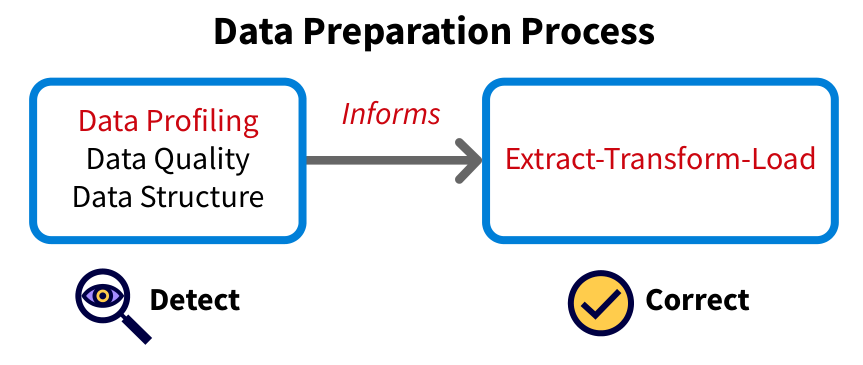
\includegraphics[width=0.95\textwidth,height=0.75\textheight,keepaspectratio]{../textbookForPractice/Figures/Ch_05/ILLUSTRATION 5.1.png}
    \end{figure}
\end{frame}

\begin{frame}{ILLUSTRATION 5.1A}

    \begin{figure}[h]
        \centering
        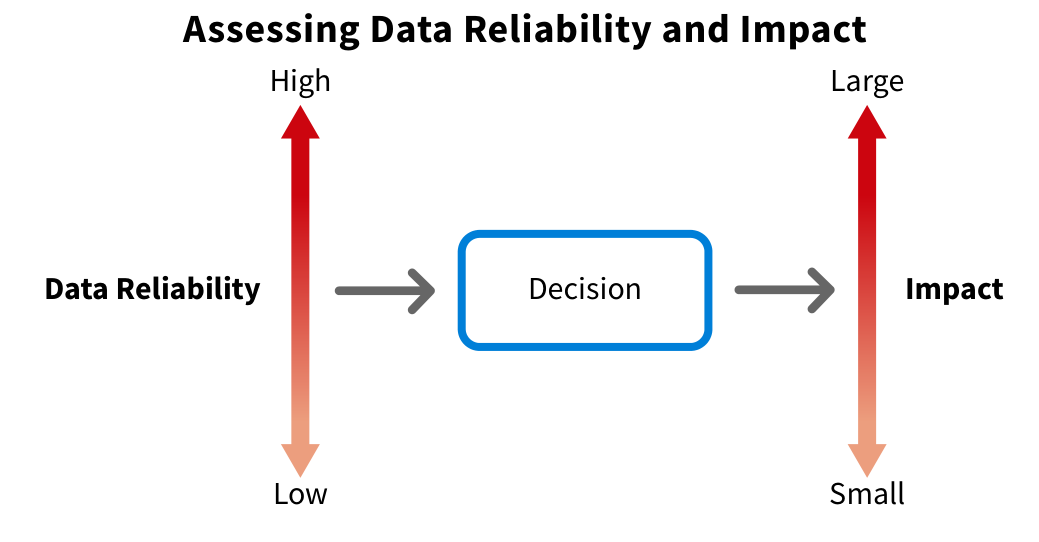
\includegraphics[width=0.95\textwidth,height=0.75\textheight,keepaspectratio]{../textbookForPractice/Figures/Ch_05/ILLUSTRATION 5.1A.png}
    \end{figure}
\end{frame}

\begin{frame}{ILLUSTRATION 5.2}

    \begin{figure}[h]
        \centering
        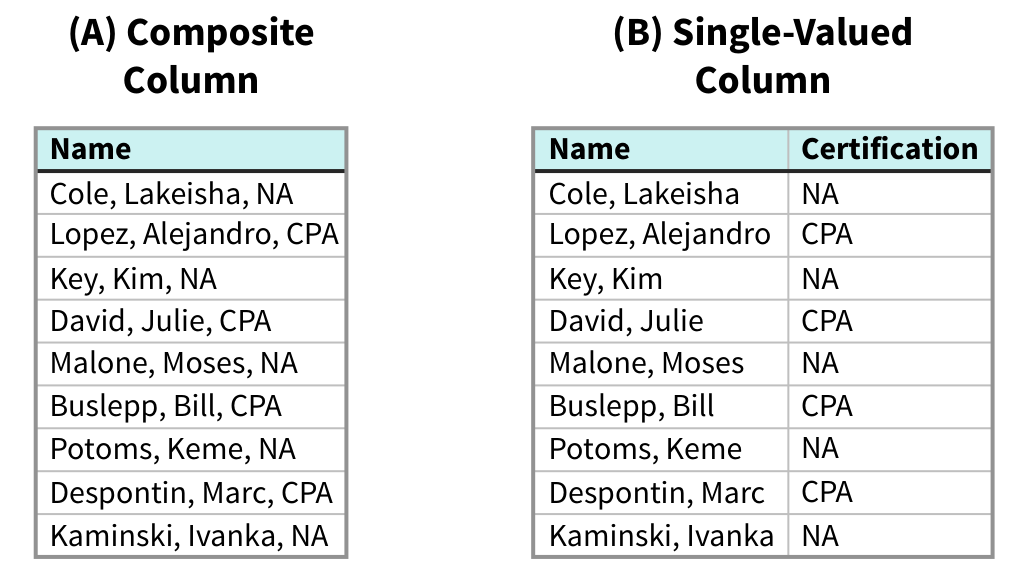
\includegraphics[width=0.95\textwidth,height=0.75\textheight,keepaspectratio]{../textbookForPractice/Figures/Ch_05/ILLUSTRATION 5.2.png}
    \end{figure}
\end{frame}

\begin{frame}{ILLUSTRATION 5.3}

    \begin{figure}[h]
        \centering
        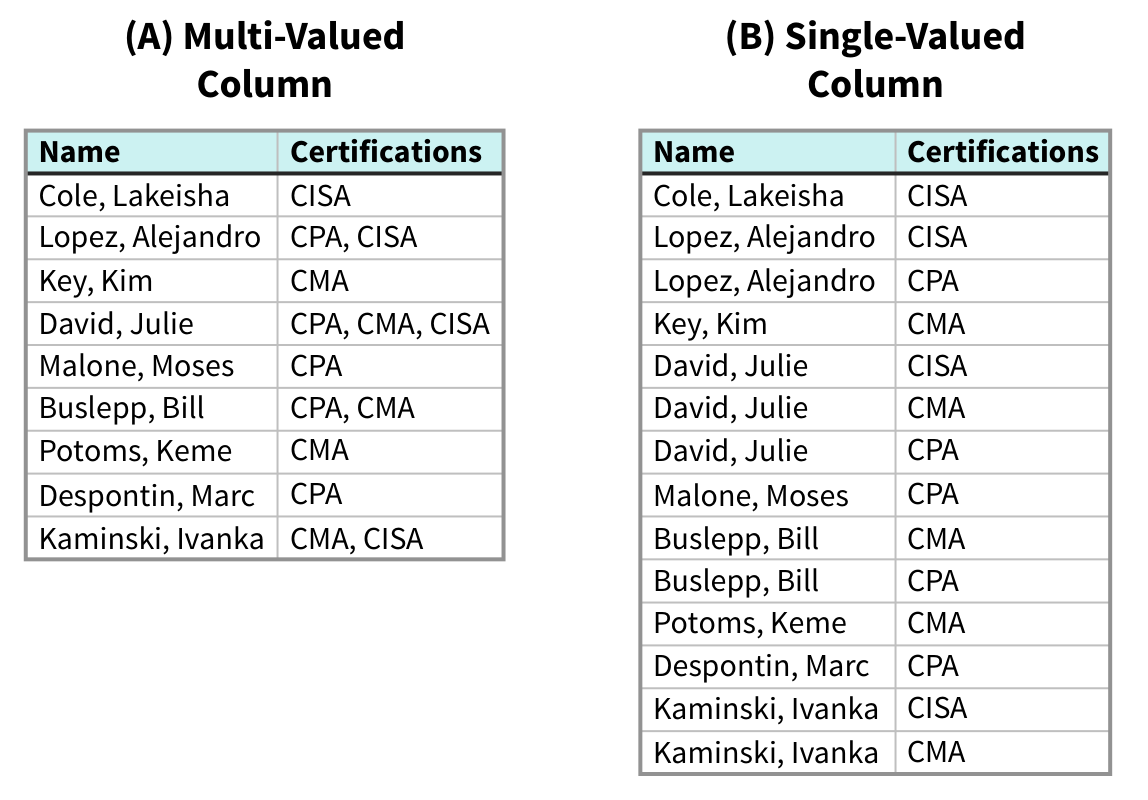
\includegraphics[width=0.95\textwidth,height=0.75\textheight,keepaspectratio]{../textbookForPractice/Figures/Ch_05/ILLUSTRATION 5.3.png}
    \end{figure}
\end{frame}

\begin{frame}{ILLUSTRATION 5.4}

    \begin{figure}[h]
        \centering
        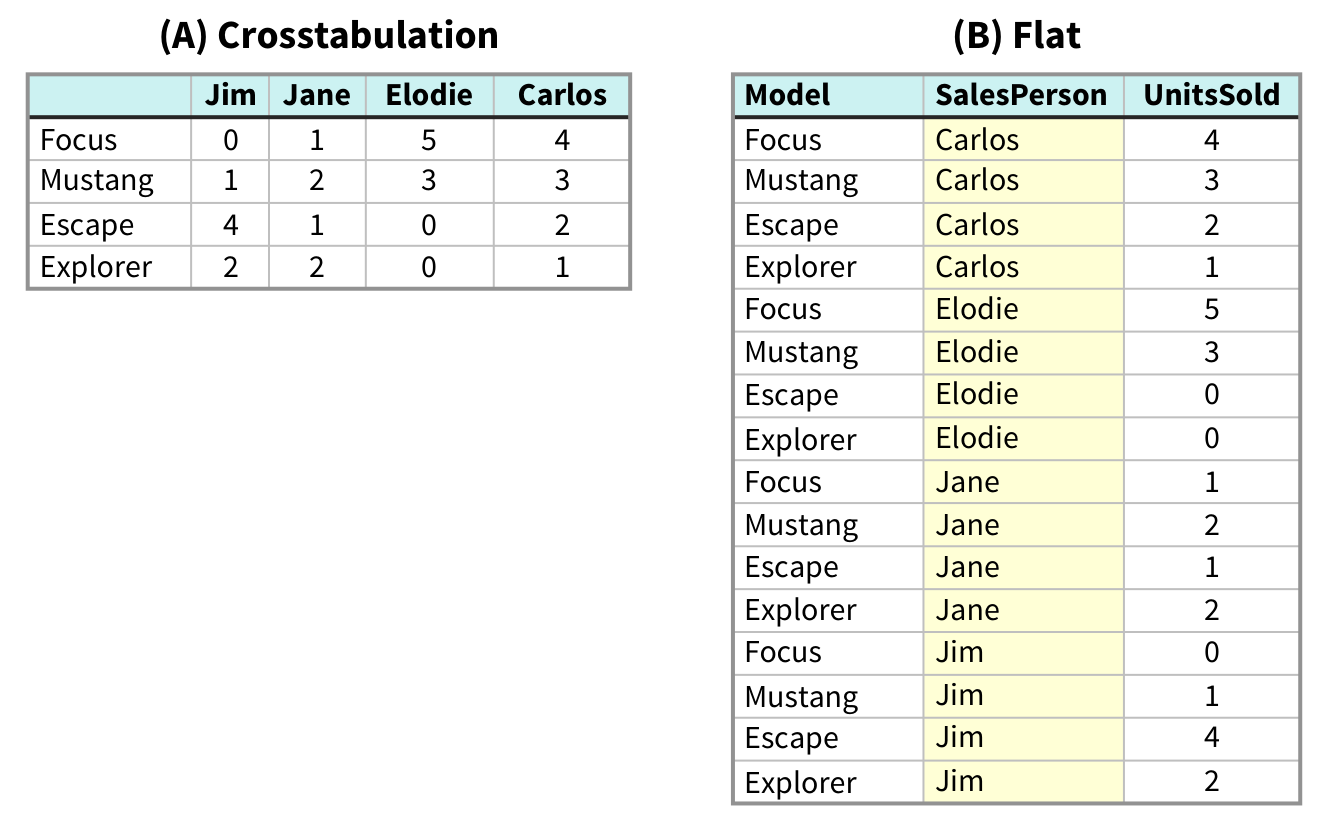
\includegraphics[width=0.95\textwidth,height=0.75\textheight,keepaspectratio]{../textbookForPractice/Figures/Ch_05/ILLUSTRATION 5.4.png}
    \end{figure}
\end{frame}

\begin{frame}{ILLUSTRATION 5.5}

    \begin{figure}[h]
        \centering
        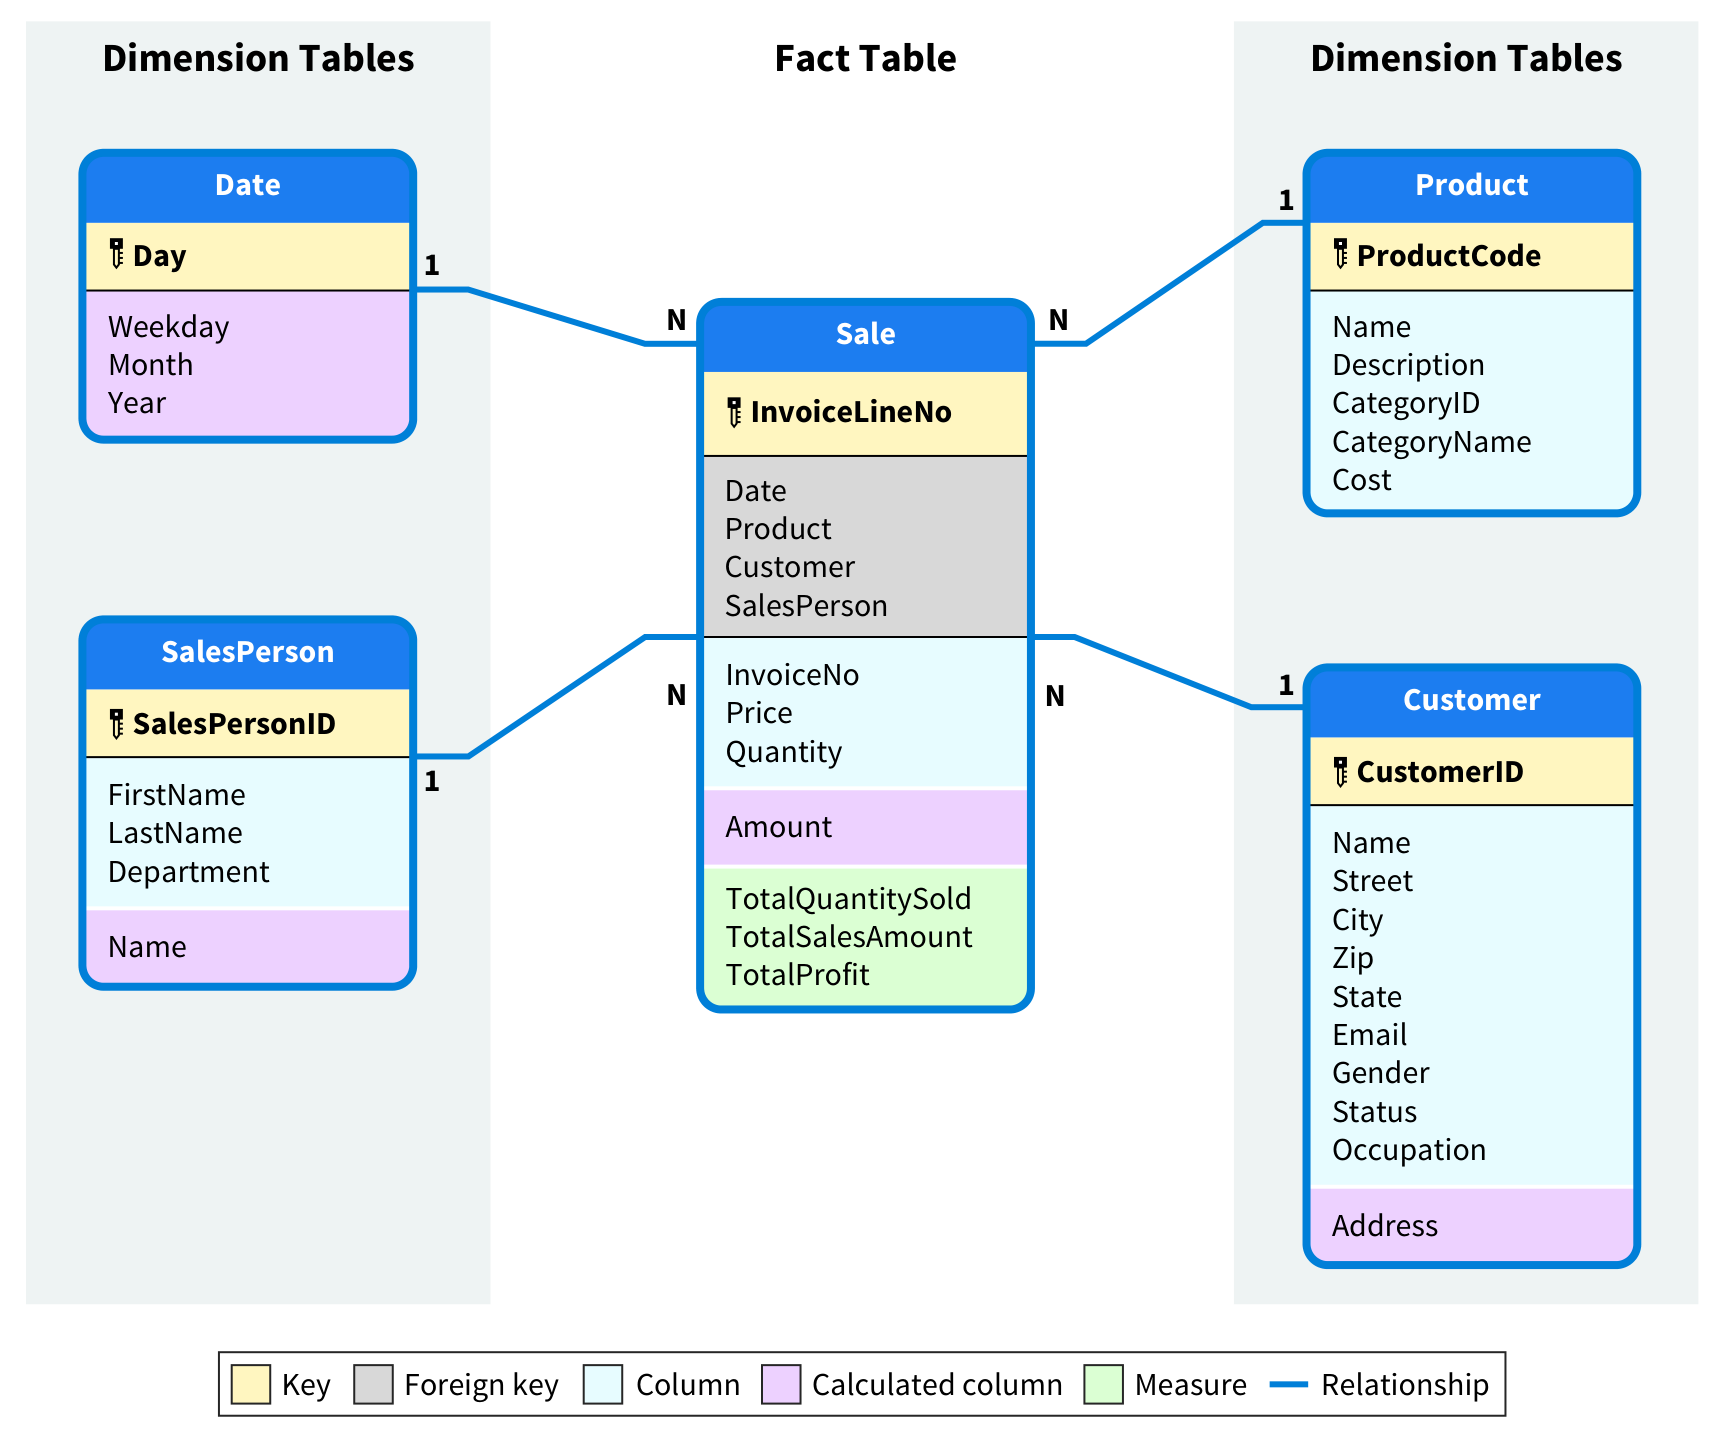
\includegraphics[width=0.95\textwidth,height=0.75\textheight,keepaspectratio]{../textbookForPractice/Figures/Ch_05/ILLUSTRATION 5.5.png}
    \end{figure}
\end{frame}

\begin{frame}{ILLUSTRATION 5.6}

    \begin{figure}[h]
        \centering
        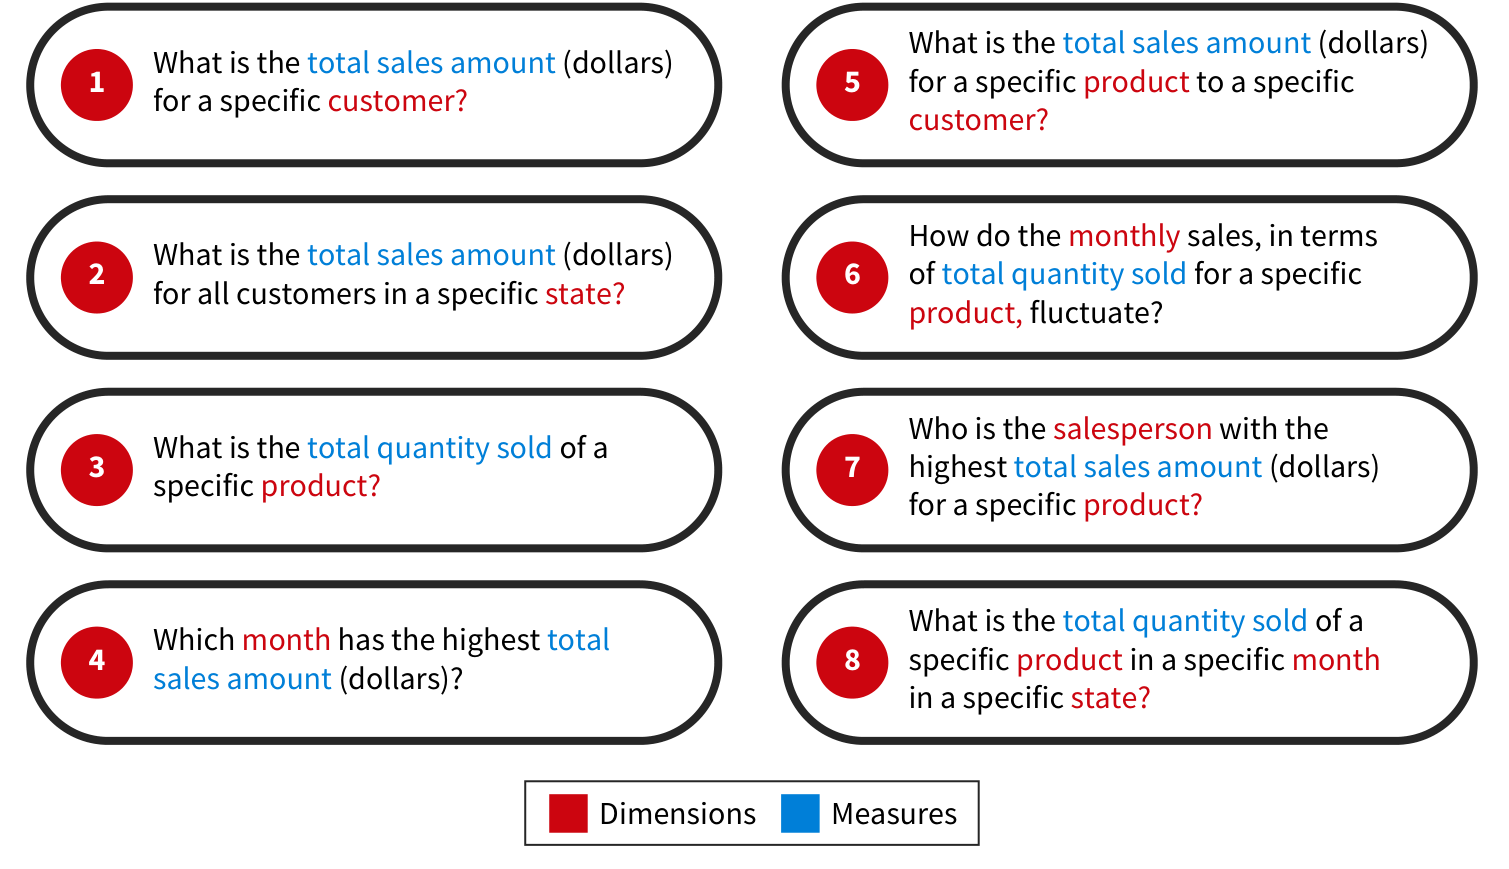
\includegraphics[width=0.95\textwidth,height=0.75\textheight,keepaspectratio]{../textbookForPractice/Figures/Ch_05/ILLUSTRATION 5.6.png}
    \end{figure}
\end{frame}

\begin{frame}{ILLUSTRATION 5.7}

    \begin{figure}[h]
        \centering
        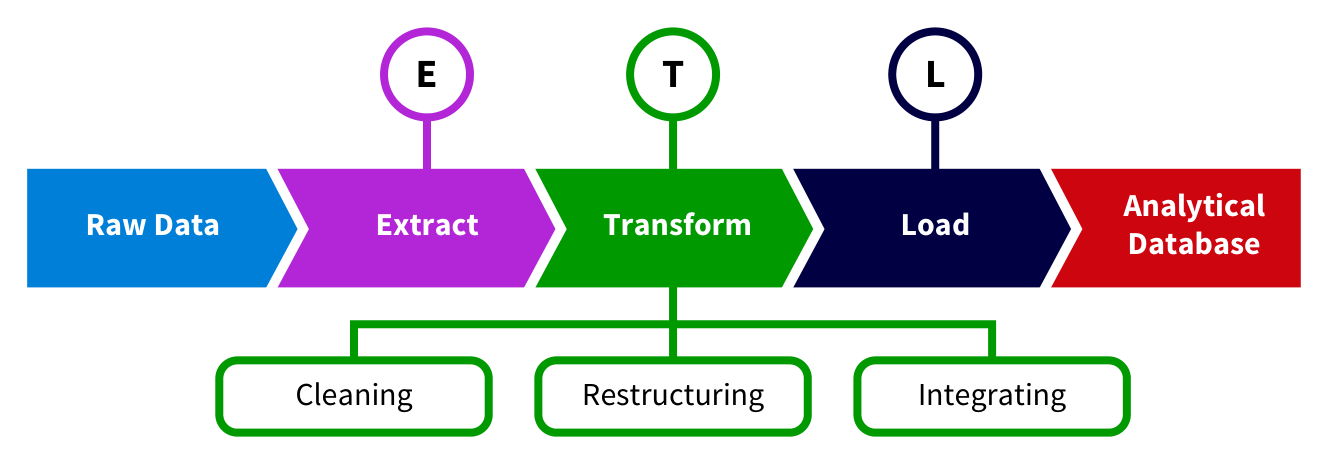
\includegraphics[width=0.95\textwidth,height=0.75\textheight,keepaspectratio]{../textbookForPractice/Figures/Ch_05/ILLUSTRATION 5.7.png}
    \end{figure}
\end{frame}

\begin{frame}{ILLUSTRATION 5.8}

    \begin{figure}[h]
        \centering
        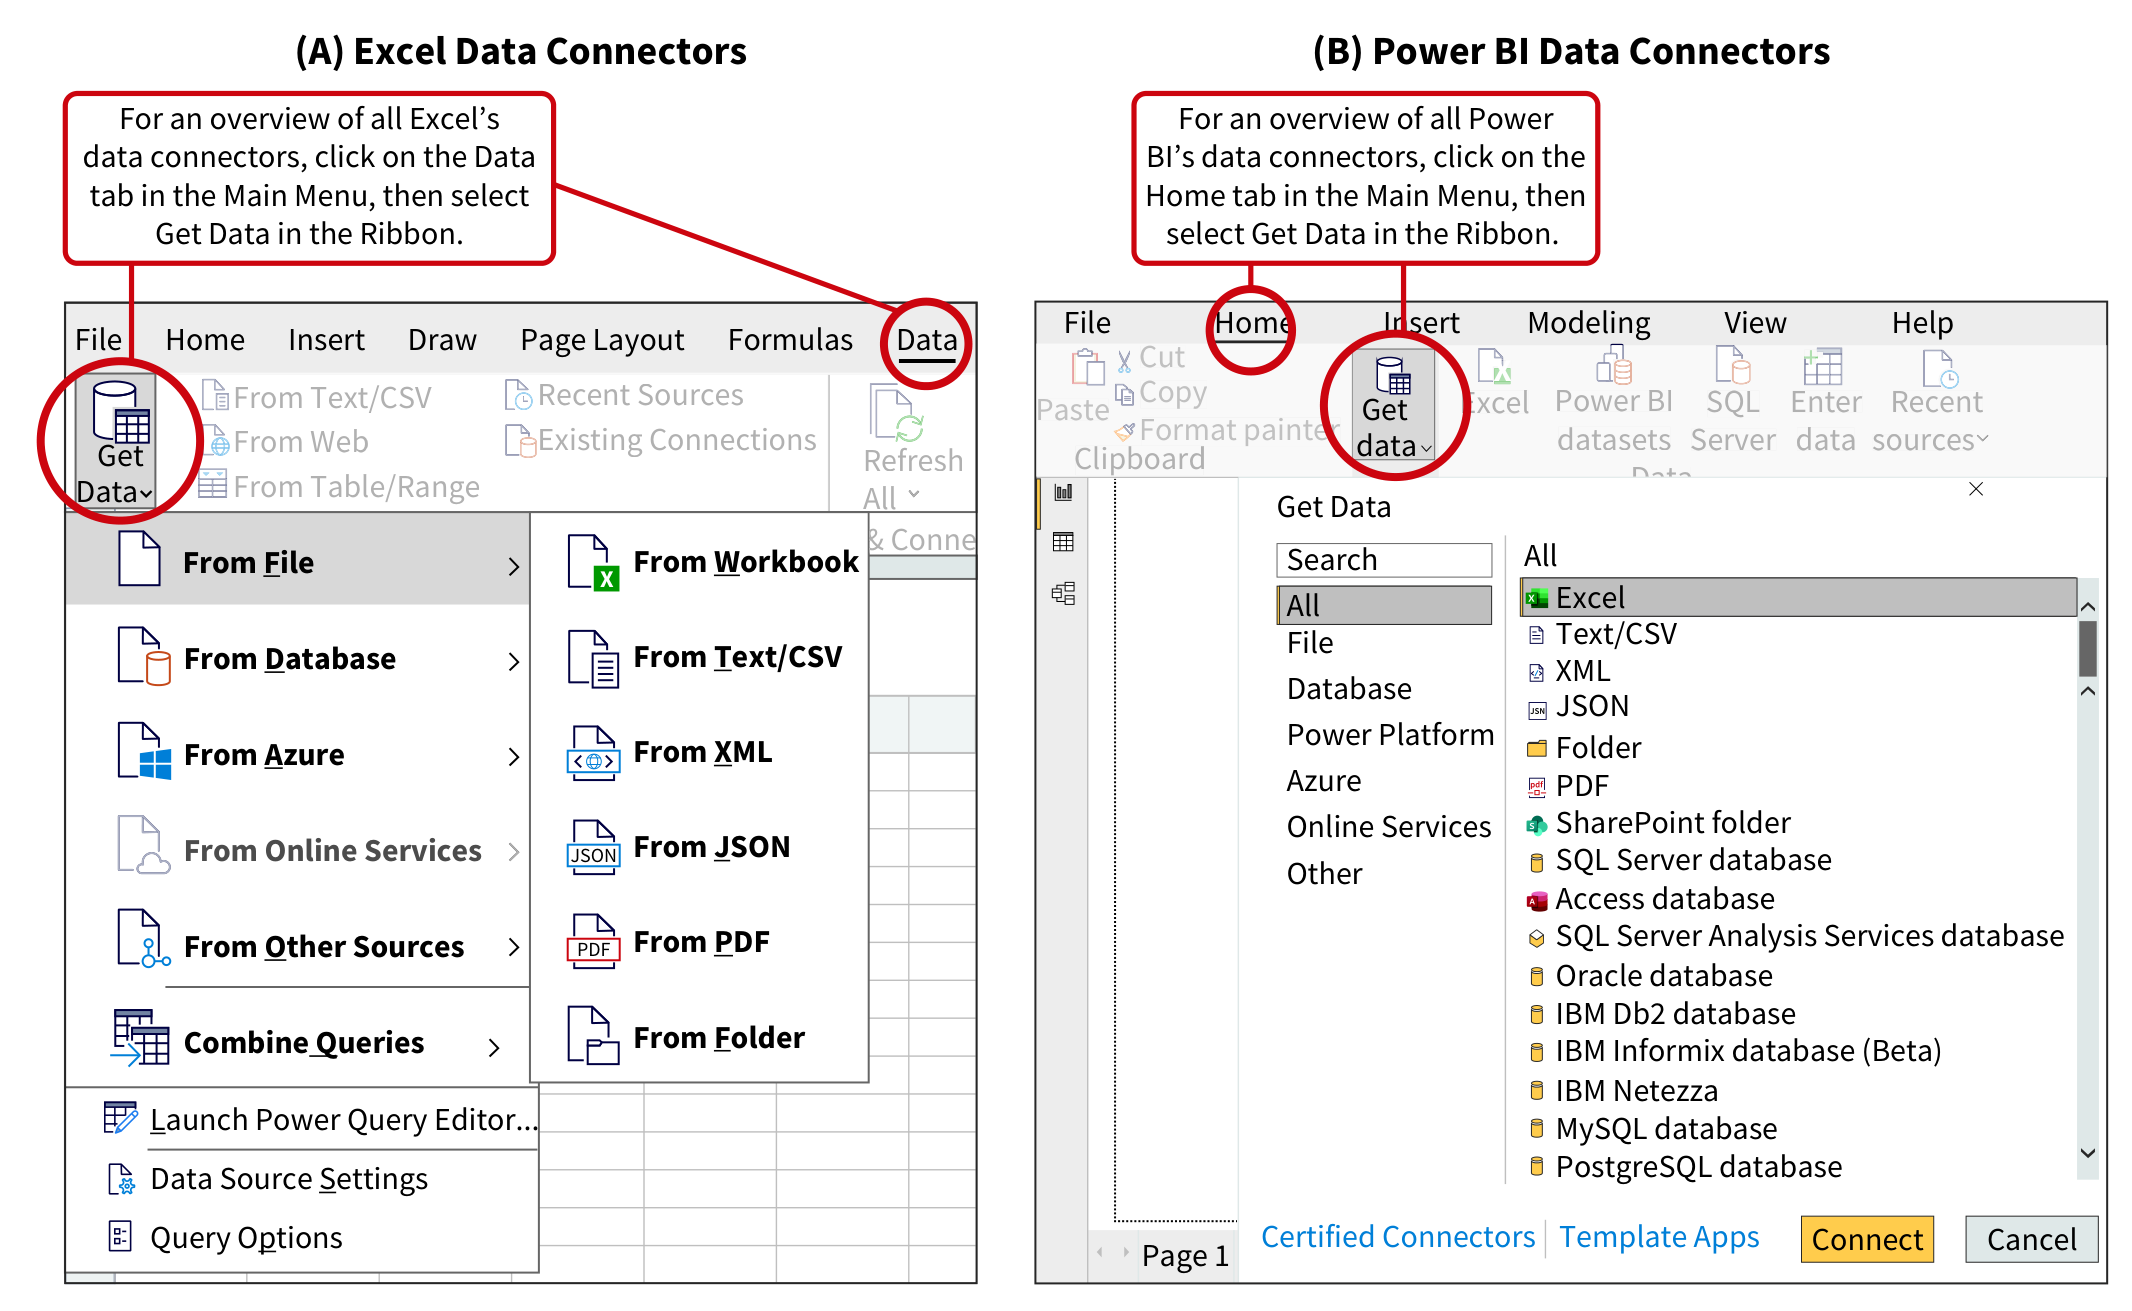
\includegraphics[width=0.95\textwidth,height=0.75\textheight,keepaspectratio]{../textbookForPractice/Figures/Ch_05/ILLUSTRATION 5.8.png}
    \end{figure}
\end{frame}

\begin{frame}{5.2 Mô tả quá trình ETL (Extract, Transform, Load)}
\begin{itemize}
    \item \textbf{E - Extract (Trích xuất):} Kéo dữ liệu từ các hệ thống nguồn (ERP, CRM, Web). Dữ liệu này thường ở dạng thô và chưa sẵn sàng để phân tích.
    \item \textbf{T - Transform (Chuyển đổi):} Là khâu quan trọng nhất. Làm sạch, tính toán lại, định dạng lại để dữ liệu phù hợp với mô hình phân tích mục tiêu.
    \item \textbf{L - Load (Tải):} Đưa dữ liệu đã được làm sạch vào kho dữ liệu (Data Warehouse) hoặc phần mềm trực quan hóa (Power BI, Tableau).
\end{itemize}
\end{frame}

\begin{frame}{ILLUSTRATION 5.9}

    \begin{figure}[h]
        \centering
        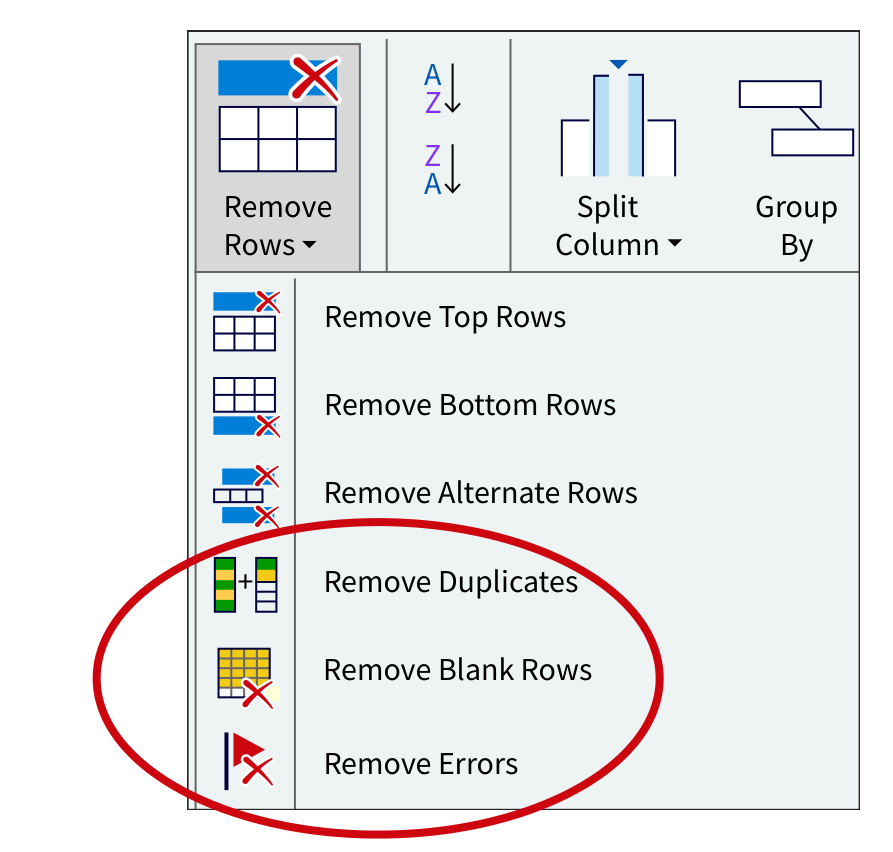
\includegraphics[width=0.95\textwidth,height=0.75\textheight,keepaspectratio]{../textbookForPractice/Figures/Ch_05/ILLUSTRATION 5.9.png}
    \end{figure}
\end{frame}

\begin{frame}{ILLUSTRATION 5.10}

    \begin{figure}[h]
        \centering
        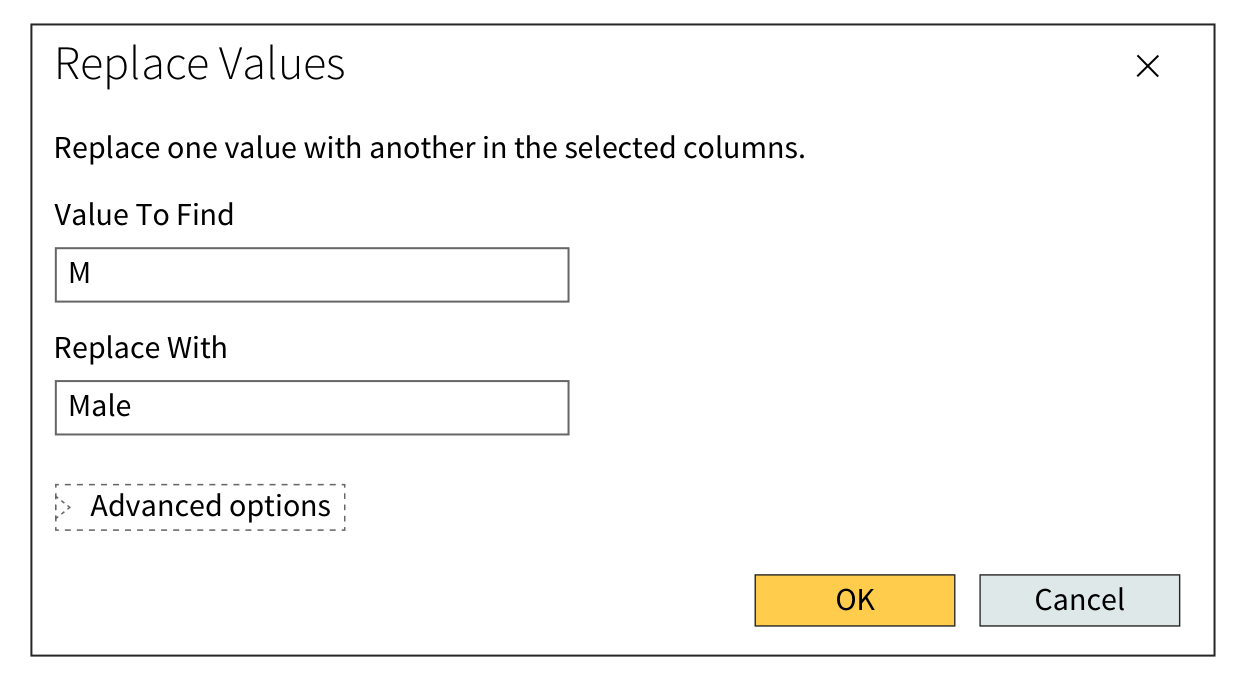
\includegraphics[width=0.95\textwidth,height=0.75\textheight,keepaspectratio]{../textbookForPractice/Figures/Ch_05/ILLUSTRATION 5.10.png}
    \end{figure}
\end{frame}

\begin{frame}{ILLUSTRATION 5.11}

    \begin{figure}[h]
        \centering
        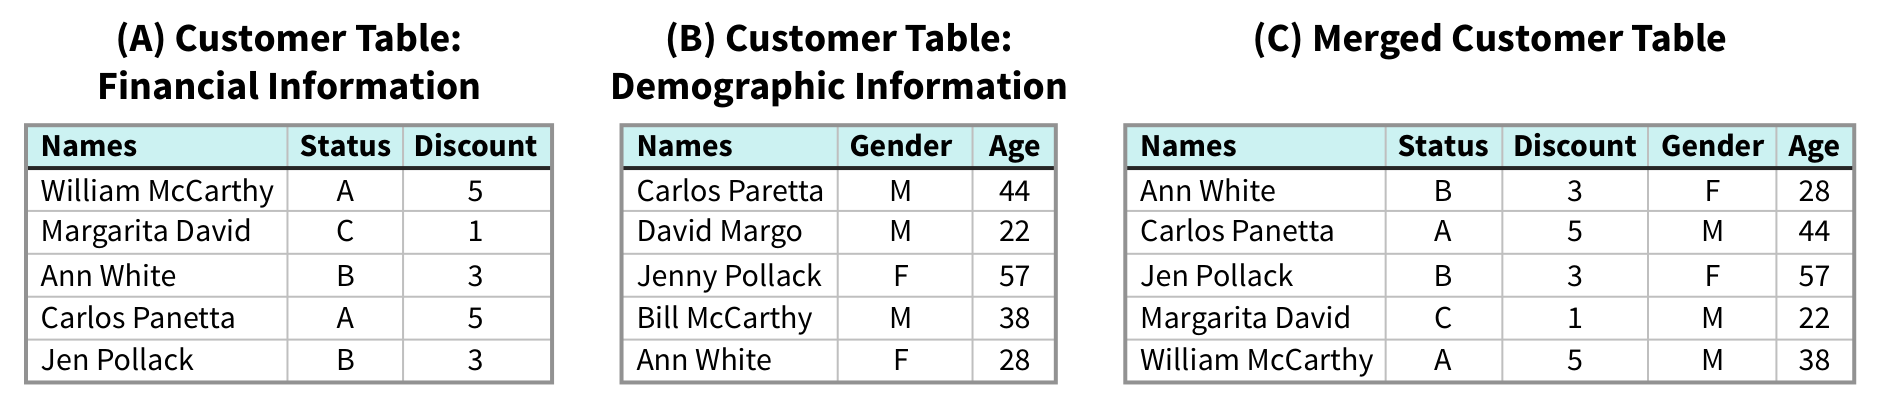
\includegraphics[width=0.95\textwidth,height=0.75\textheight,keepaspectratio]{../textbookForPractice/Figures/Ch_05/ILLUSTRATION 5.11.png}
    \end{figure}
\end{frame}

\begin{frame}{ILLUSTRATION 5.12}

    \begin{figure}[h]
        \centering
        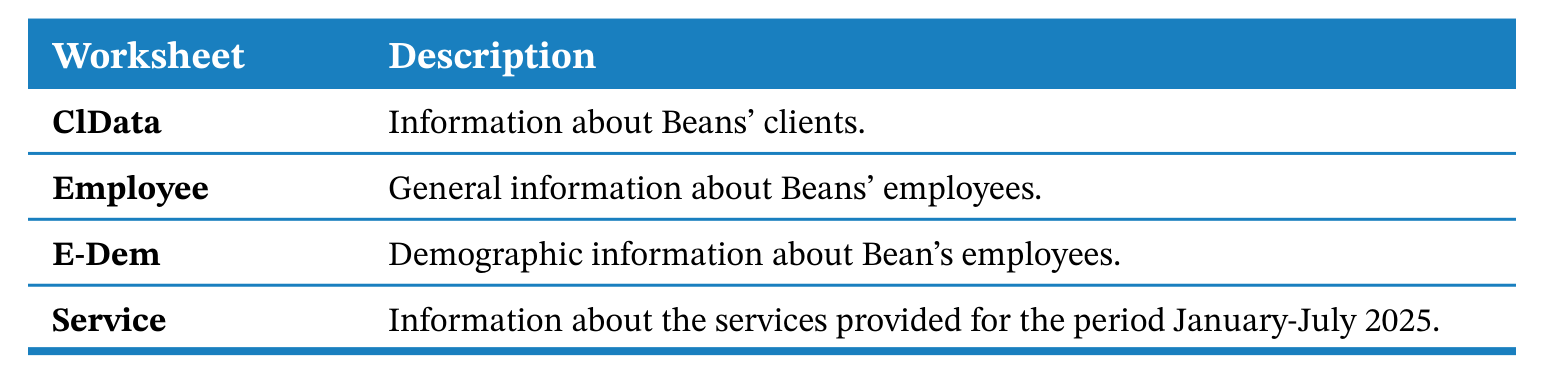
\includegraphics[width=0.95\textwidth,height=0.75\textheight,keepaspectratio]{../textbookForPractice/Figures/Ch_05/ILLUSTRATION 5.12.png}
    \end{figure}
\end{frame}

\begin{frame}{ILLUSTRATION 5.13A}

    \begin{figure}[h]
        \centering
        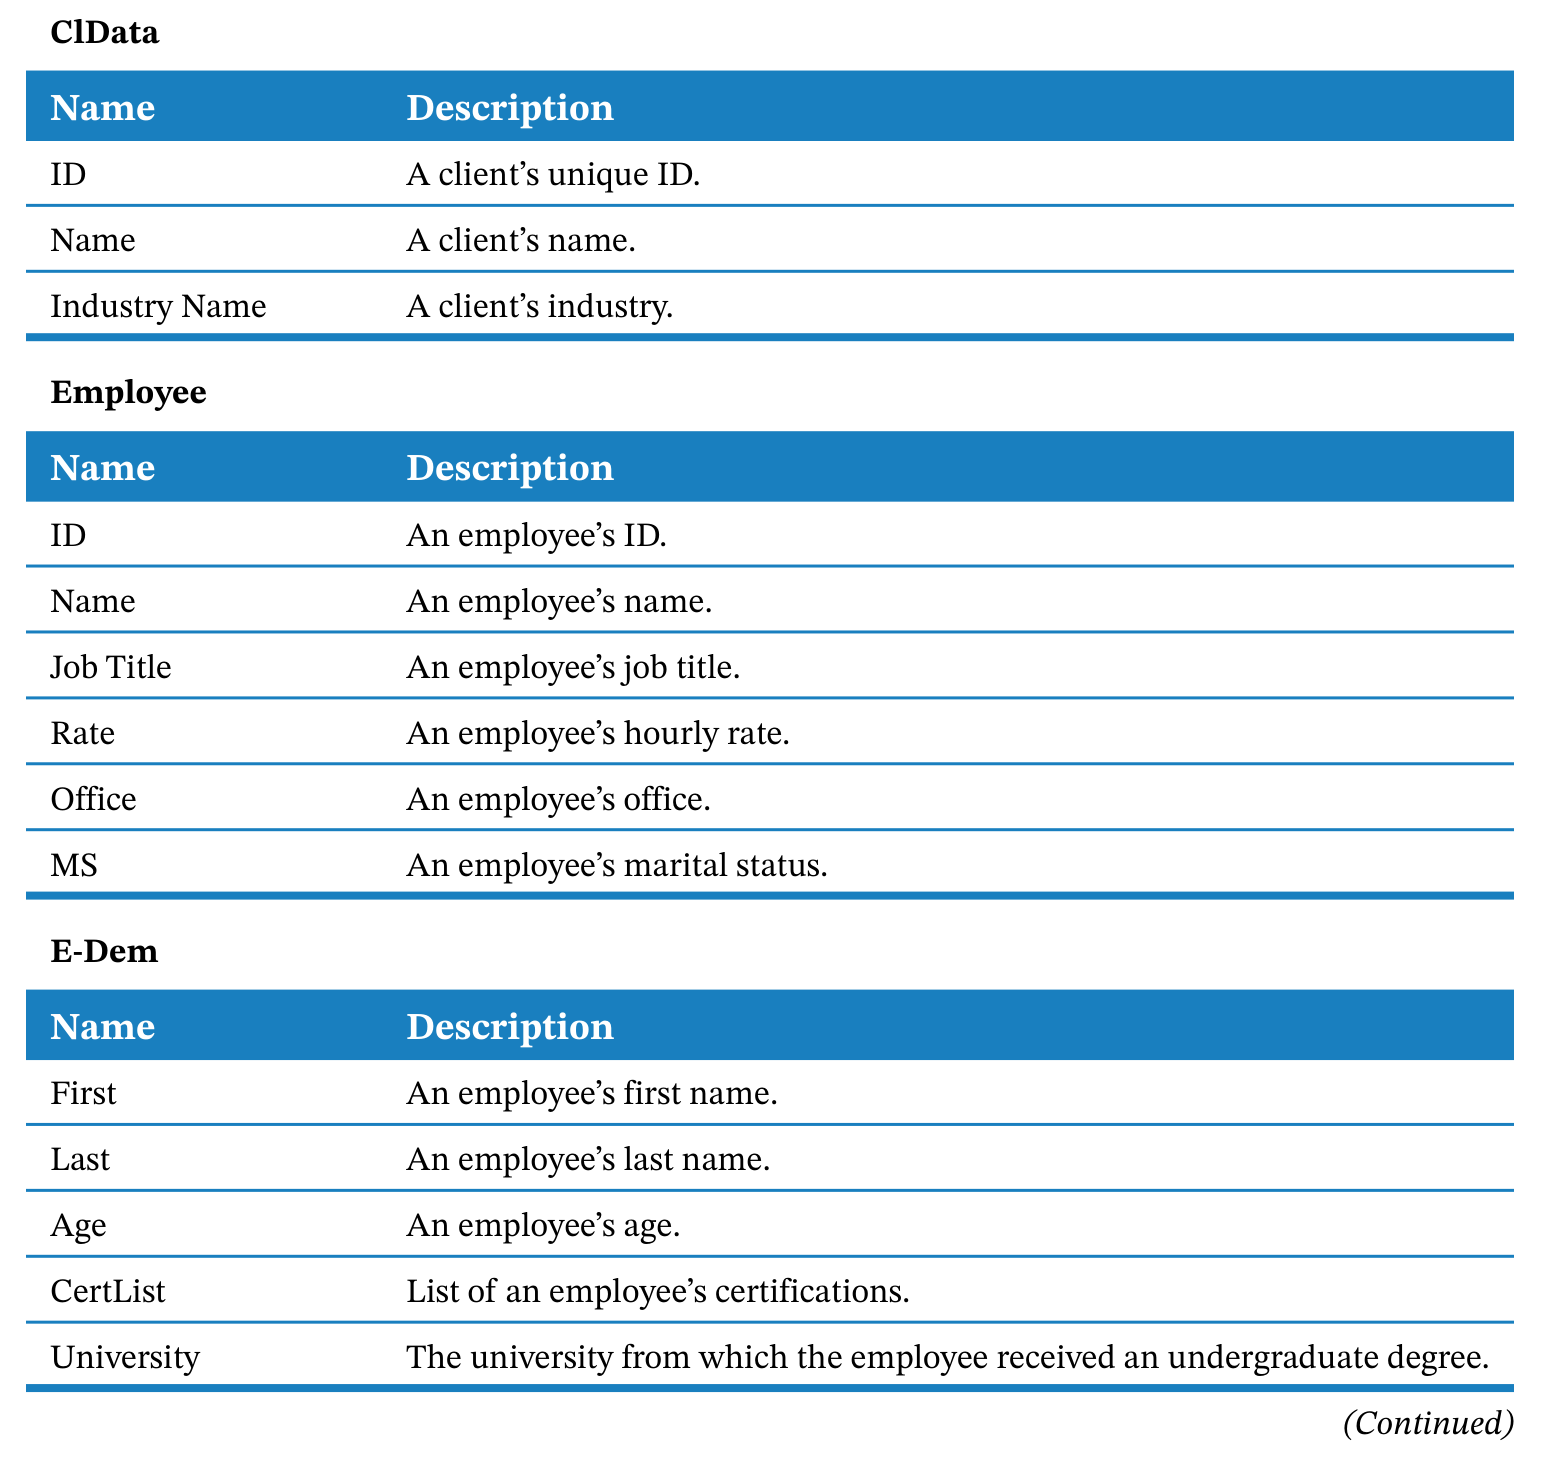
\includegraphics[width=0.95\textwidth,height=0.75\textheight,keepaspectratio]{../textbookForPractice/Figures/Ch_05/ILLUSTRATION 5.13A.png}
    \end{figure}
\end{frame}

\begin{frame}{ILLUSTRATION 5.13B}

    \begin{figure}[h]
        \centering
        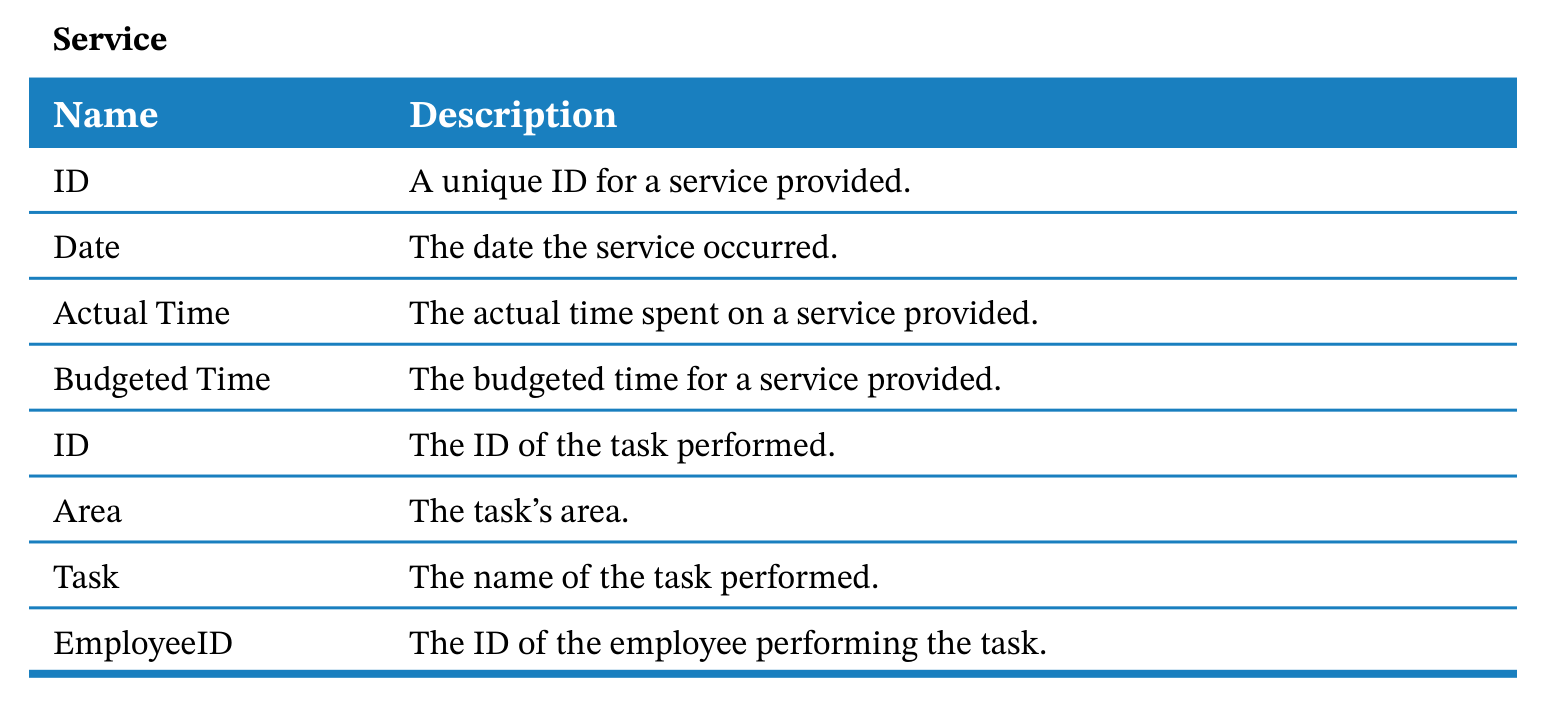
\includegraphics[width=0.95\textwidth,height=0.75\textheight,keepaspectratio]{../textbookForPractice/Figures/Ch_05/ILLUSTRATION 5.13B.png}
    \end{figure}
\end{frame}

\begin{frame}{ILLUSTRATION 5.14}

    \begin{figure}[h]
        \centering
        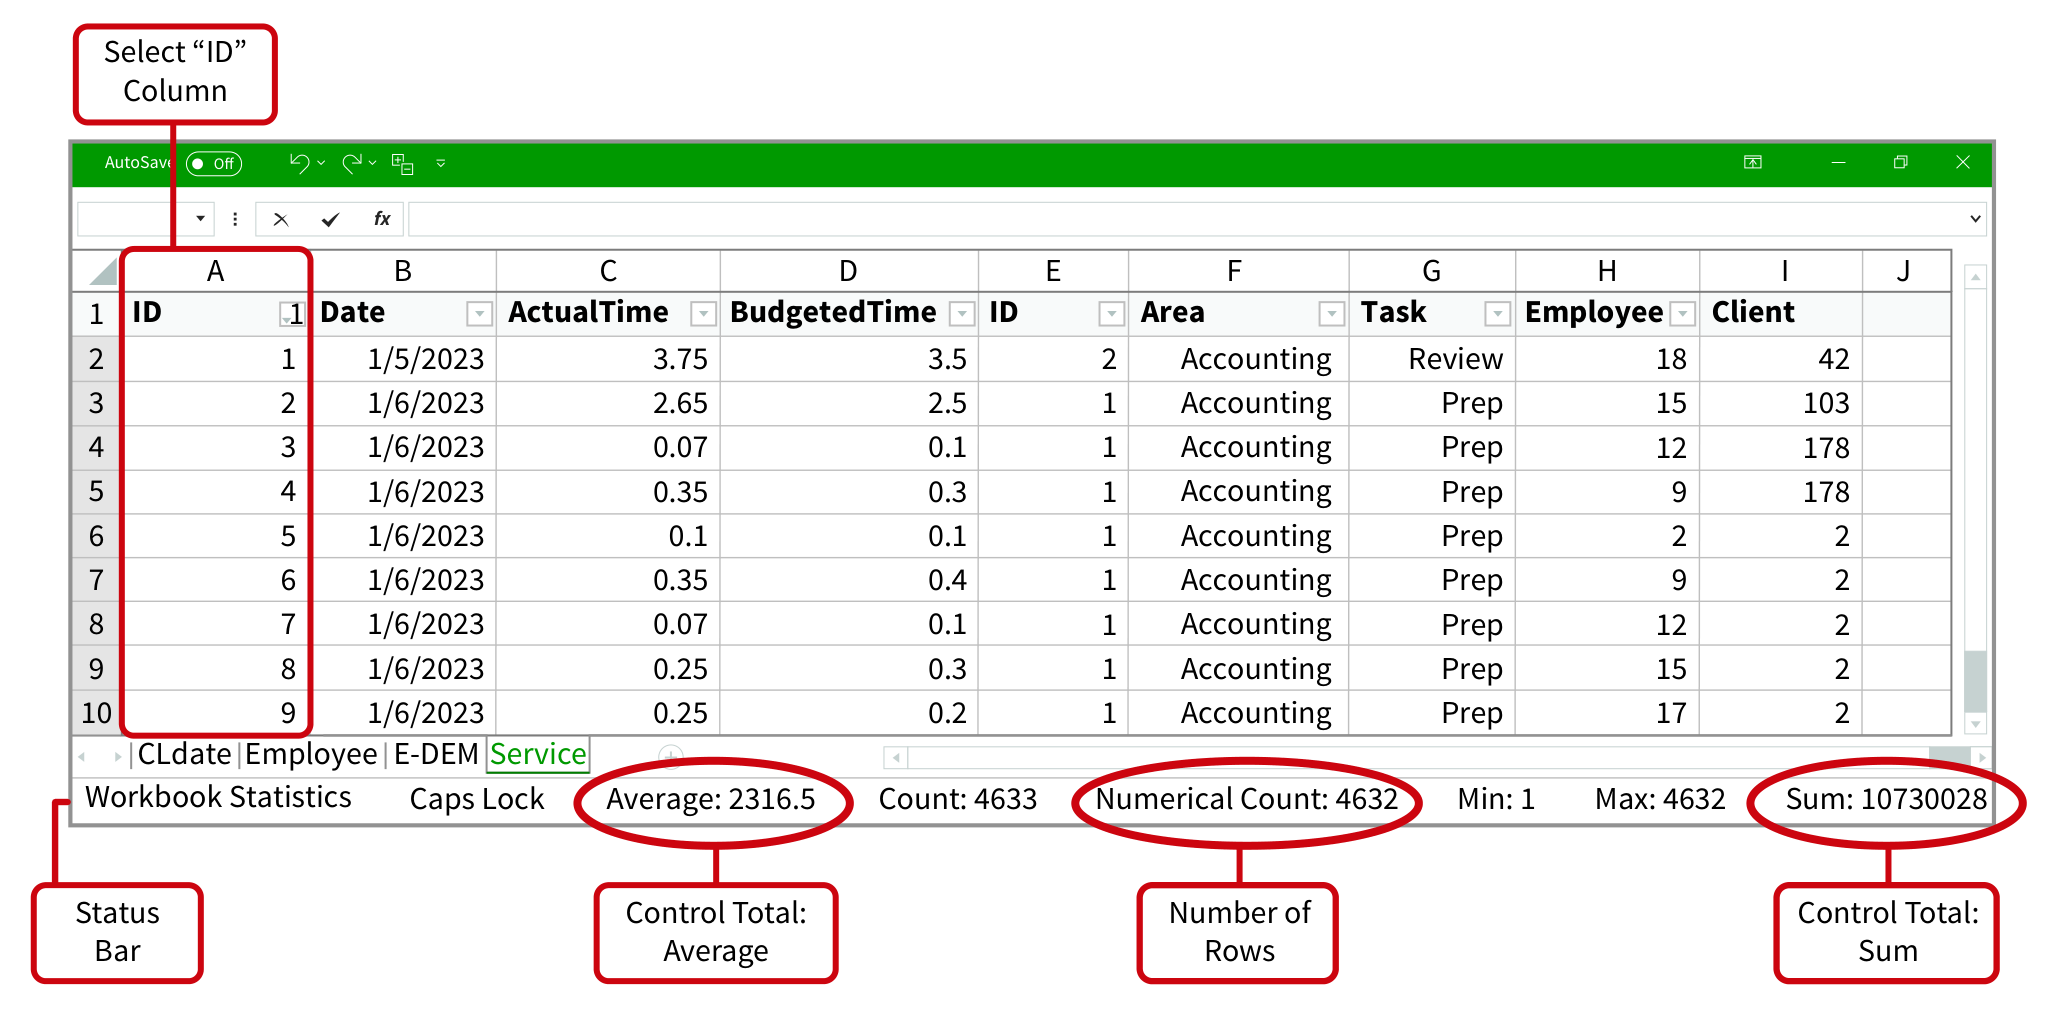
\includegraphics[width=0.95\textwidth,height=0.75\textheight,keepaspectratio]{../textbookForPractice/Figures/Ch_05/ILLUSTRATION 5.14.png}
    \end{figure}
\end{frame}

\begin{frame}{ILLUSTRATION 5.15}

    \begin{figure}[h]
        \centering
        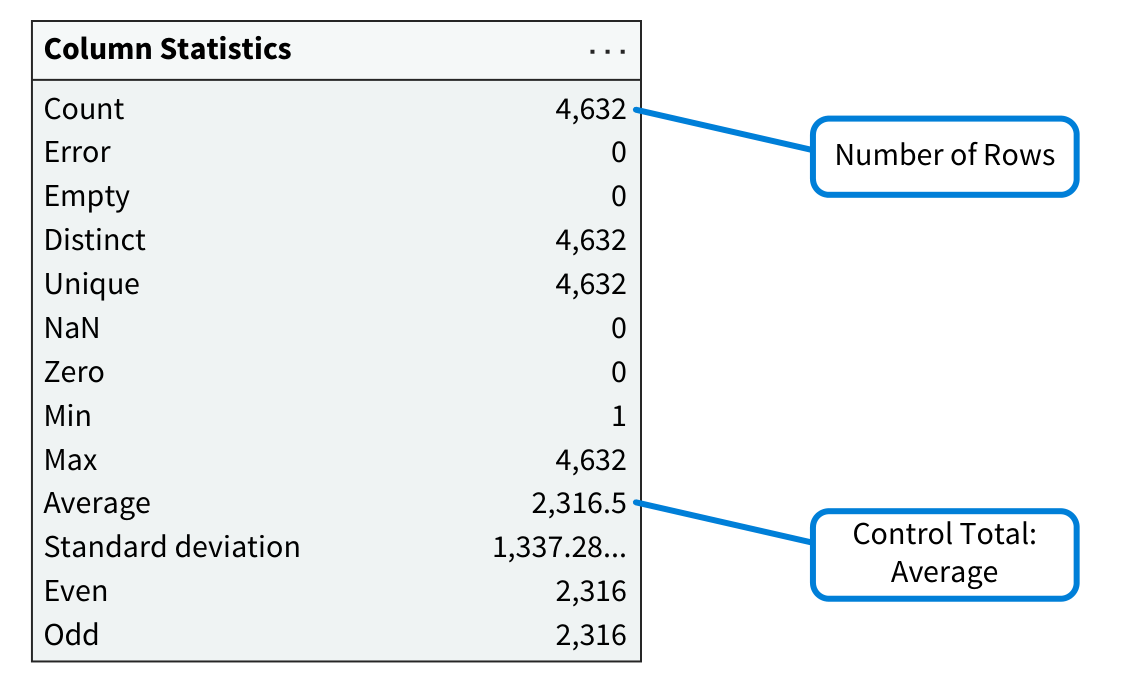
\includegraphics[width=0.95\textwidth,height=0.75\textheight,keepaspectratio]{../textbookForPractice/Figures/Ch_05/ILLUSTRATION 5.15.png}
    \end{figure}
\end{frame}

\begin{frame}{ILLUSTRATION 5.16}

    \begin{figure}[h]
        \centering
        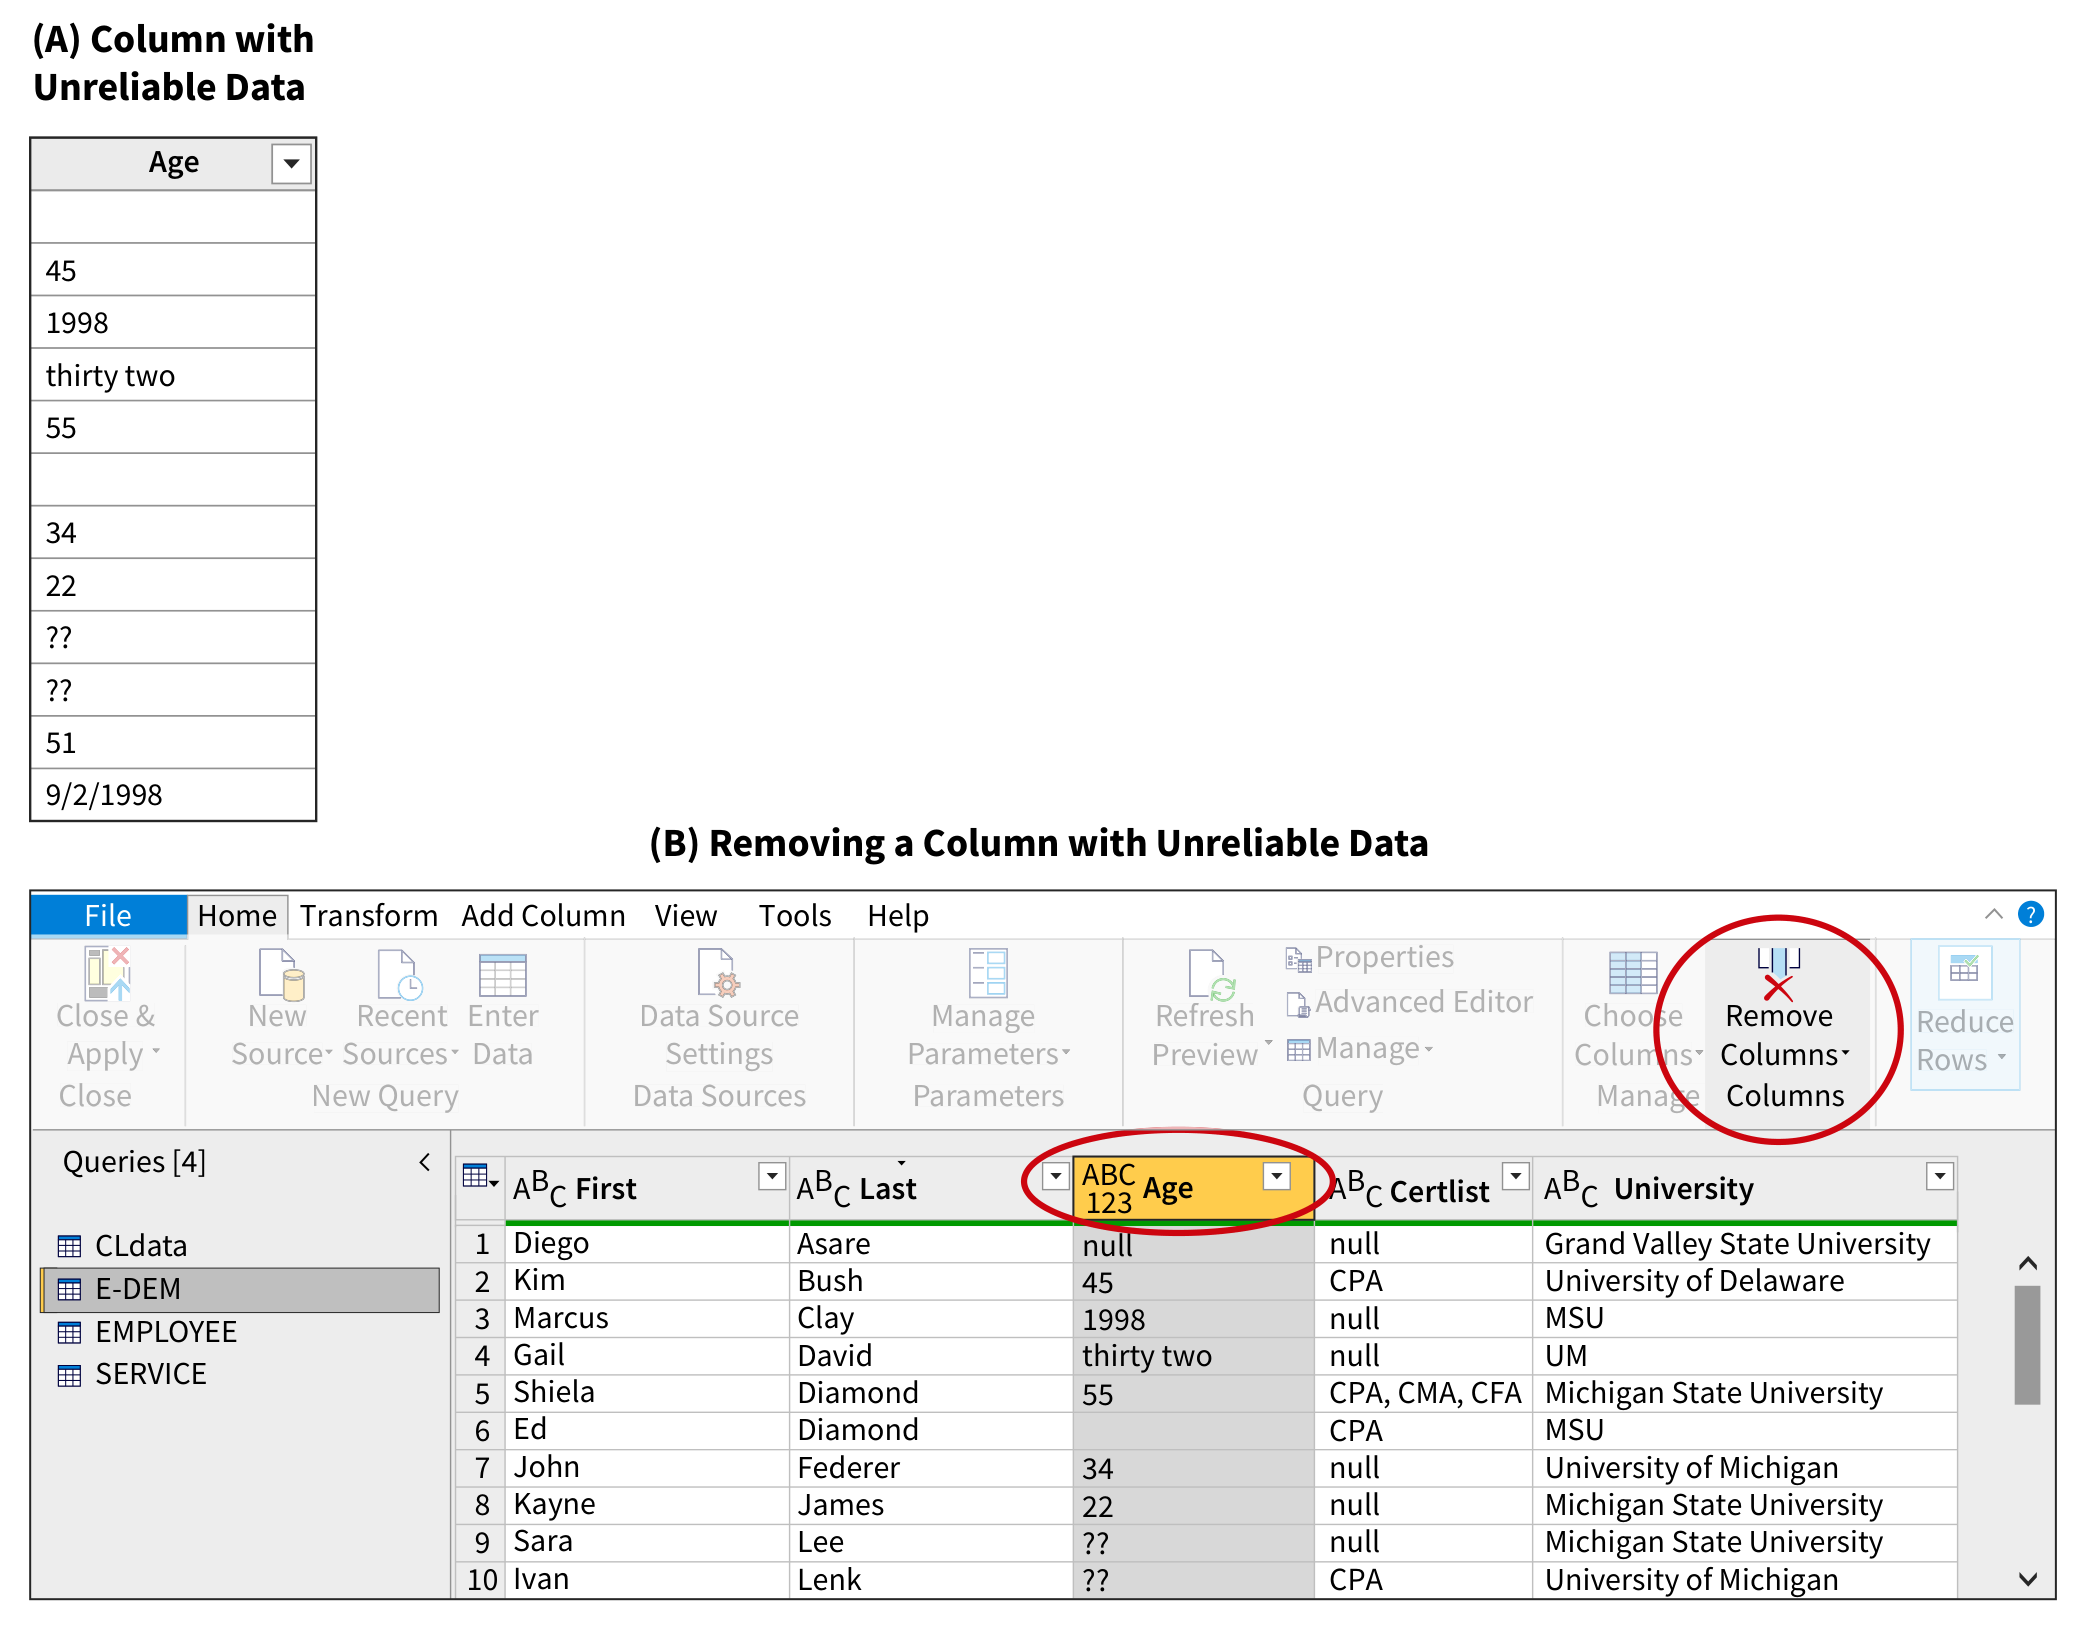
\includegraphics[width=0.95\textwidth,height=0.75\textheight,keepaspectratio]{../textbookForPractice/Figures/Ch_05/ILLUSTRATION 5.16.png}
    \end{figure}
\end{frame}

\begin{frame}{5.3 Áp dụng các mẫu để Trích xuất Dữ liệu (Extraction Patterns)}
\begin{itemize}
    \item \textbf{Mẫu trích xuất toàn bộ (Full Extraction):} 
    \begin{itemize}
        \item Rút toàn bộ dữ liệu từ nguồn ở mỗi lần thực hiện. Phù hợp với các bảng dữ liệu nhỏ (Ví dụ: Danh mục khách hàng).
    \end{itemize}
    \item \textbf{Mẫu trích xuất tăng dần (Incremental Extraction):}
    \begin{itemize}
        \item Chỉ trích xuất những dữ liệu mới được tạo hoặc bị thay đổi kể từ lần trích xuất cuối cùng. Giúp tiết kiệm băng thông và tài nguyên hệ thống (Ví dụ: Dữ liệu giao dịch bán hàng hàng ngày).
    \end{itemize}
\end{itemize}
\end{frame}

\begin{frame}{ILLUSTRATION 5.17}

    \begin{figure}[h]
        \centering
        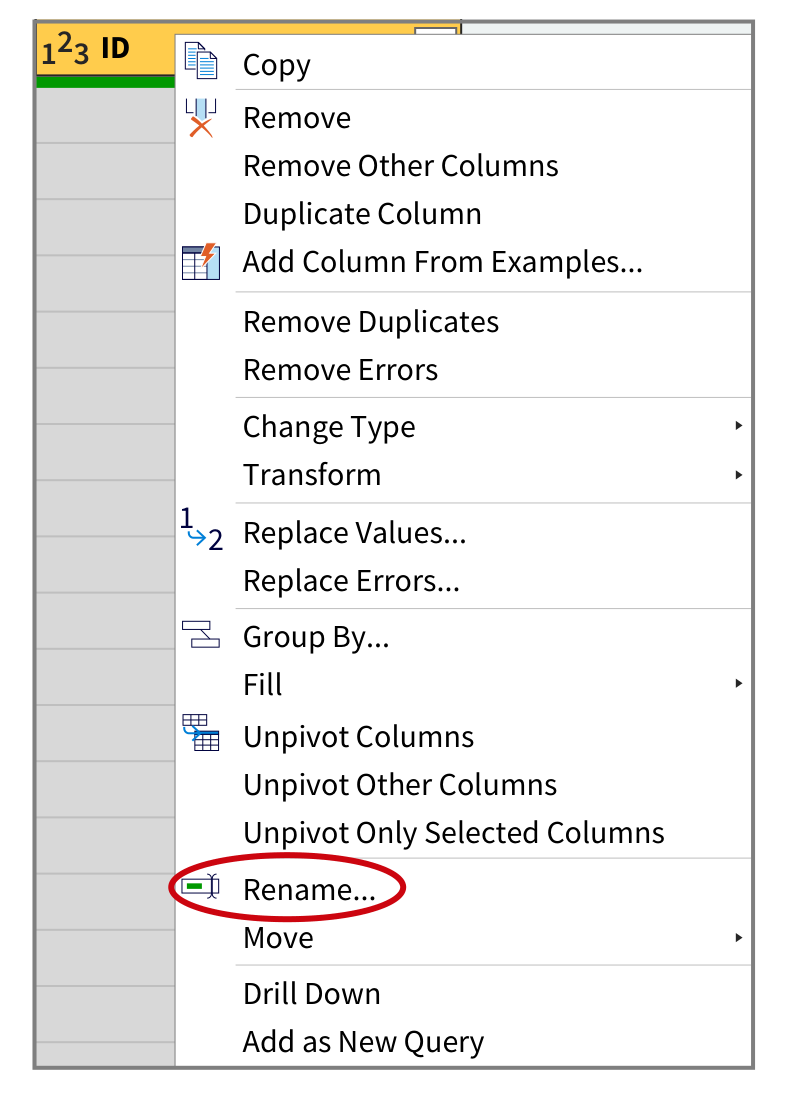
\includegraphics[width=0.95\textwidth,height=0.75\textheight,keepaspectratio]{../textbookForPractice/Figures/Ch_05/ILLUSTRATION 5.17.png}
    \end{figure}
\end{frame}

\begin{frame}{ILLUSTRATION 5.18}

    \begin{figure}[h]
        \centering
        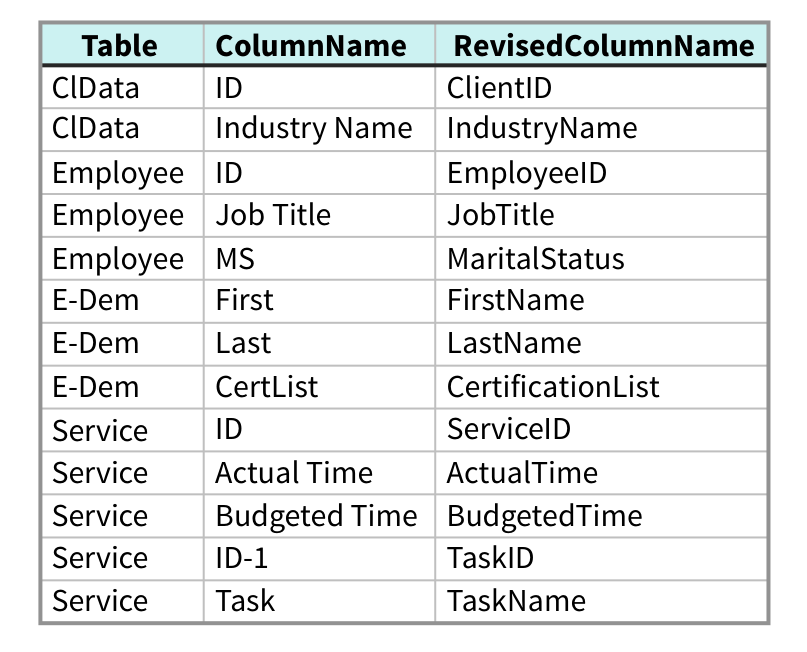
\includegraphics[width=0.95\textwidth,height=0.75\textheight,keepaspectratio]{../textbookForPractice/Figures/Ch_05/ILLUSTRATION 5.18.png}
    \end{figure}
\end{frame}

\begin{frame}{ILLUSTRATION 5.19}

    \begin{figure}[h]
        \centering
        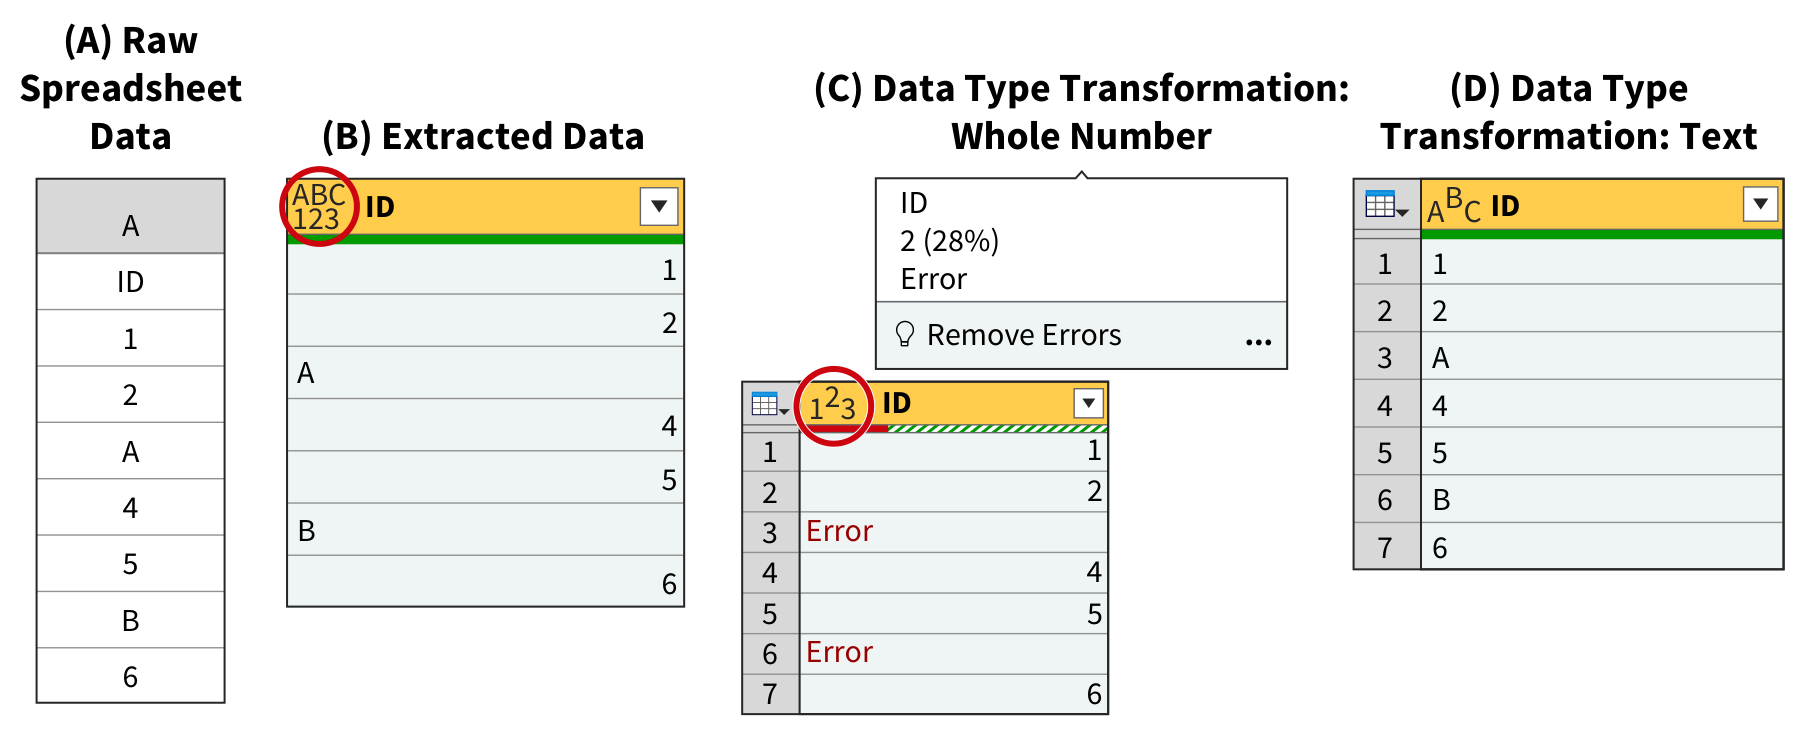
\includegraphics[width=0.95\textwidth,height=0.75\textheight,keepaspectratio]{../textbookForPractice/Figures/Ch_05/ILLUSTRATION 5.19.png}
    \end{figure}
\end{frame}

\begin{frame}{ILLUSTRATION 5.20}

    \begin{figure}[h]
        \centering
        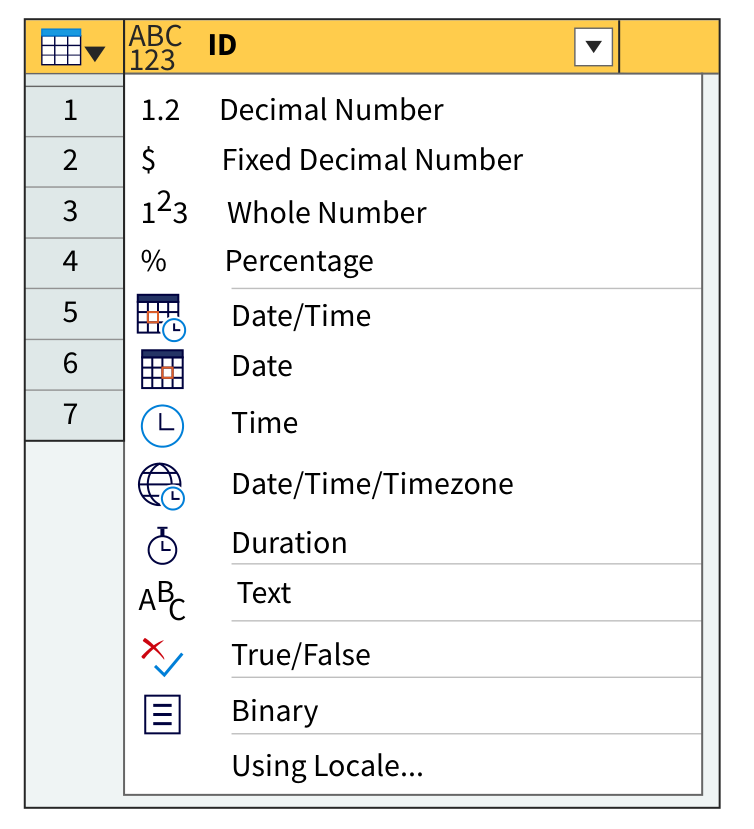
\includegraphics[width=0.95\textwidth,height=0.75\textheight,keepaspectratio]{../textbookForPractice/Figures/Ch_05/ILLUSTRATION 5.20.png}
    \end{figure}
\end{frame}

\begin{frame}{ILLUSTRATION 5.21}

    \begin{figure}[h]
        \centering
        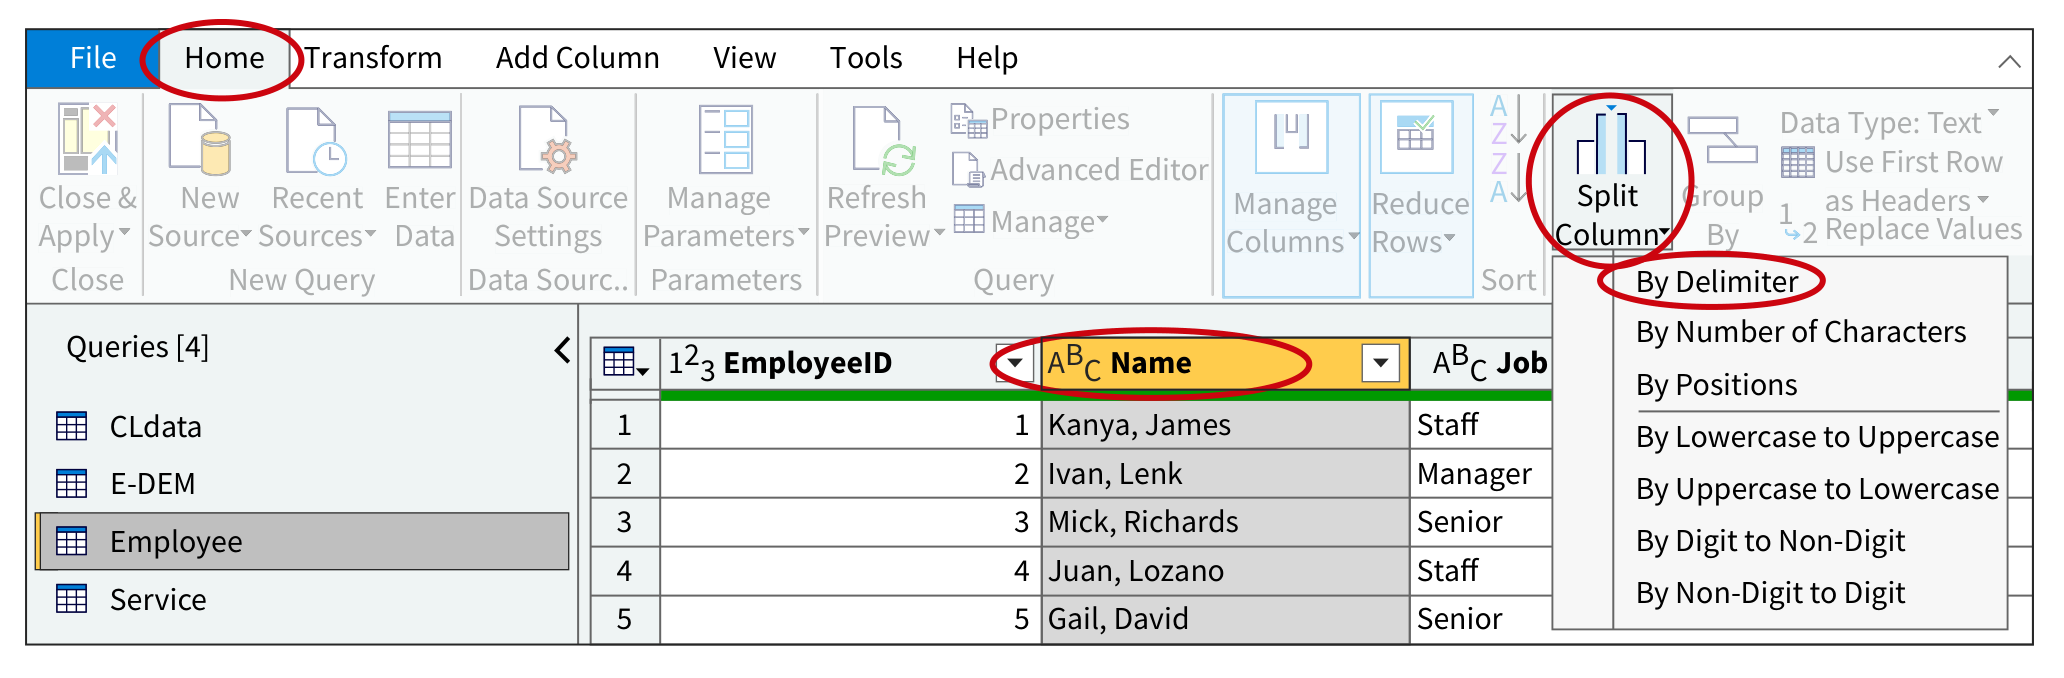
\includegraphics[width=0.95\textwidth,height=0.75\textheight,keepaspectratio]{../textbookForPractice/Figures/Ch_05/ILLUSTRATION 5.21.png}
    \end{figure}
\end{frame}

\begin{frame}{ILLUSTRATION 5.22}

    \begin{figure}[h]
        \centering
        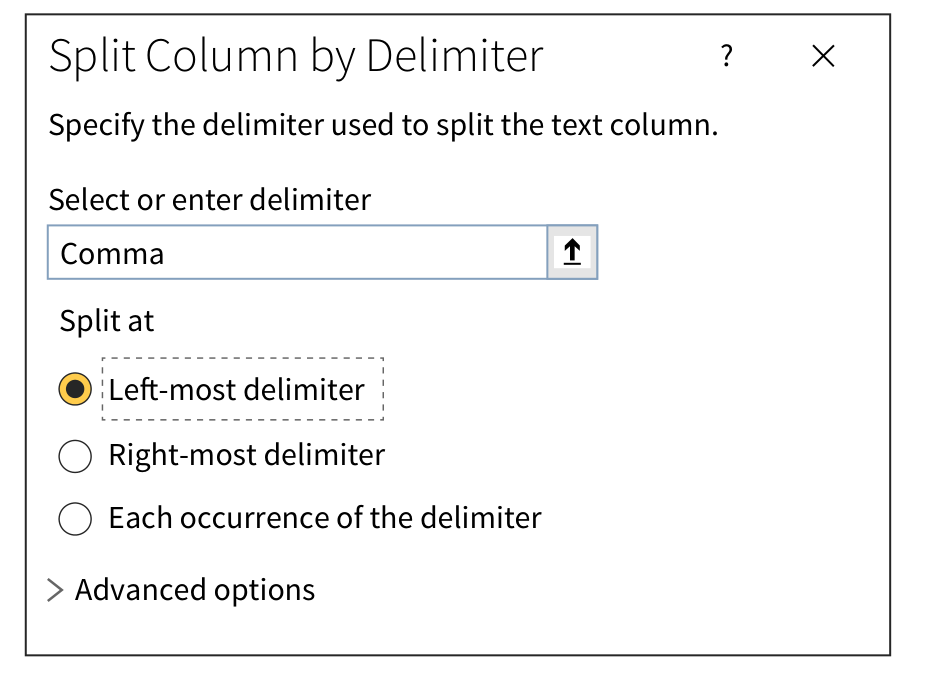
\includegraphics[width=0.95\textwidth,height=0.75\textheight,keepaspectratio]{../textbookForPractice/Figures/Ch_05/ILLUSTRATION 5.22.png}
    \end{figure}
\end{frame}

\begin{frame}{ILLUSTRATION 5.23}

    \begin{figure}[h]
        \centering
        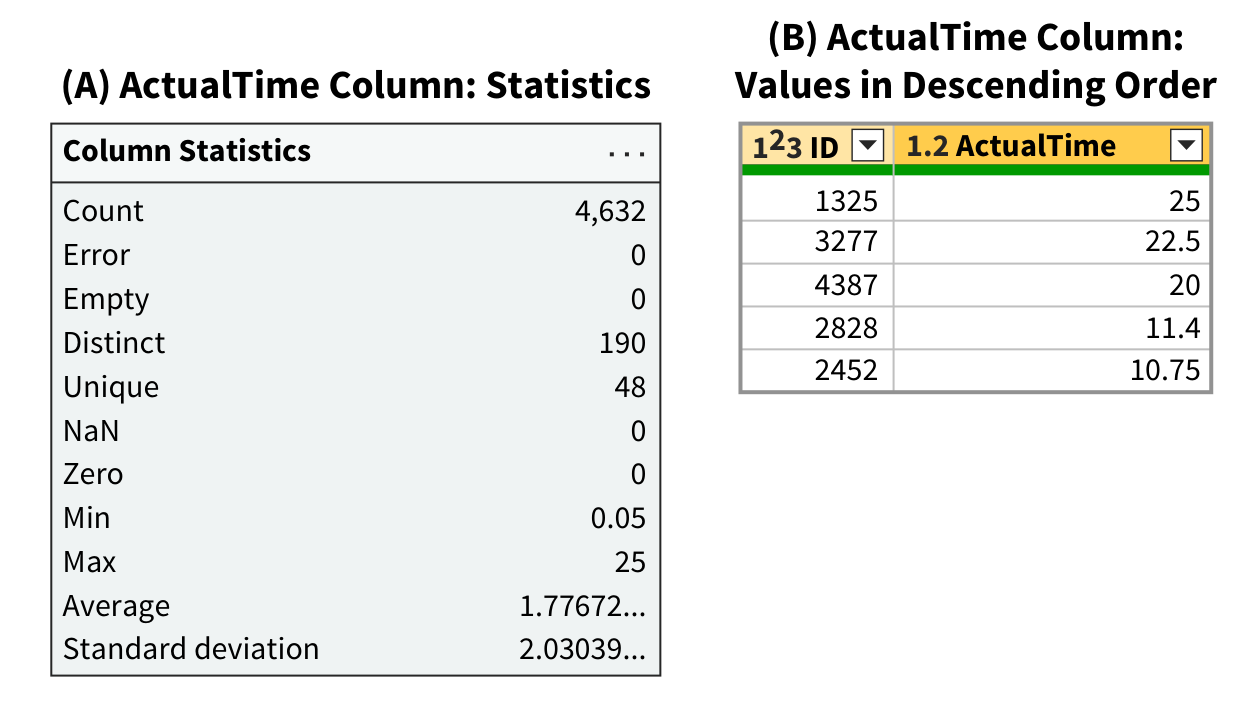
\includegraphics[width=0.95\textwidth,height=0.75\textheight,keepaspectratio]{../textbookForPractice/Figures/Ch_05/ILLUSTRATION 5.23.png}
    \end{figure}
\end{frame}

\begin{frame}{ILLUSTRATION 5.24}

    \begin{figure}[h]
        \centering
        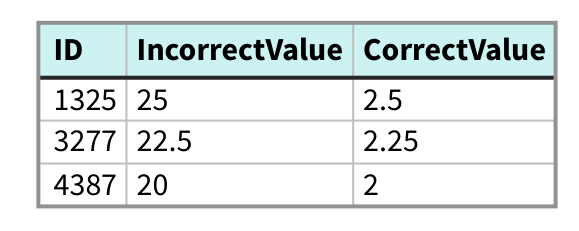
\includegraphics[width=0.95\textwidth,height=0.75\textheight,keepaspectratio]{../textbookForPractice/Figures/Ch_05/ILLUSTRATION 5.24.png}
    \end{figure}
\end{frame}

\begin{frame}{ILLUSTRATION 5.25}

    \begin{figure}[h]
        \centering
        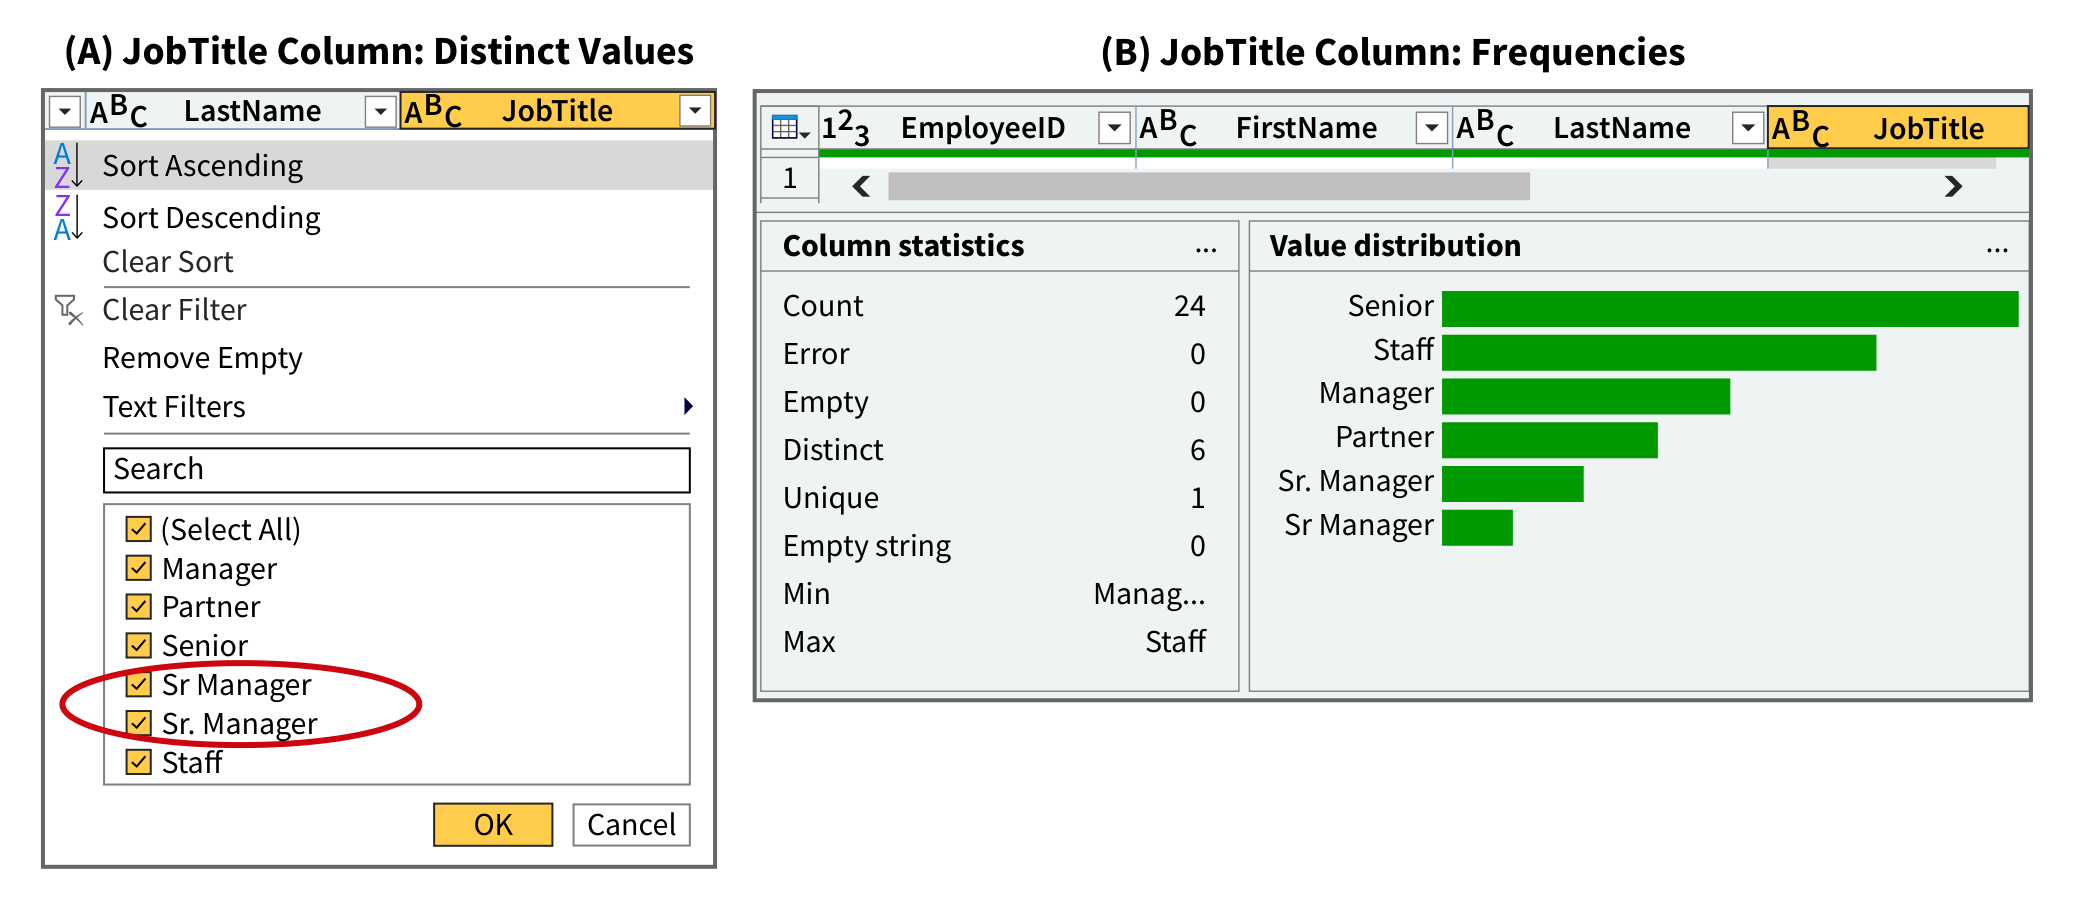
\includegraphics[width=0.95\textwidth,height=0.75\textheight,keepaspectratio]{../textbookForPractice/Figures/Ch_05/ILLUSTRATION 5.25.png}
    \end{figure}
\end{frame}

\begin{frame}{5.4 Áp dụng mẫu để Chuyển đổi Cột (Column Transformation)}
\begin{itemize}
    \item \textbf{1. Làm sạch (Cleaning):} Xóa khoảng trắng thừa (Trim), sửa lỗi chính tả.
    \item \textbf{2. Định dạng (Formatting):} Đổi định dạng tiền tệ (VND sang USD), định dạng ngày tháng (MM/DD/YYYY sang DD/MM/YYYY).
    \item \textbf{3. Tách cột (Splitting):} Tách cột "Họ và Tên" thành hai cột "Họ" và "Tên".
    \item \textbf{4. Ghép cột (Concatenating):} Nối "Mã vùng" và "Số điện thoại".
    \item \textbf{5. Rút trích (Extracting):} Lấy tên miền từ địa chỉ Email.
    \item \textbf{6. Tính toán (Calculated):} Cột "Thành tiền" = "Số lượng" $\times$ "Đơn giá".
\end{itemize}
\end{frame}

\begin{frame}{ILLUSTRATION 5.26}

    \begin{figure}[h]
        \centering
        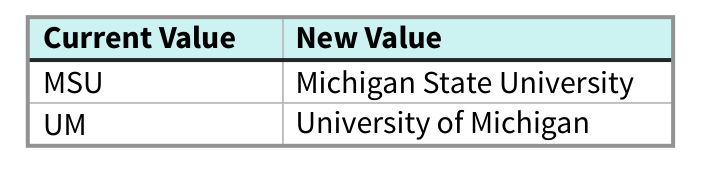
\includegraphics[width=0.95\textwidth,height=0.75\textheight,keepaspectratio]{../textbookForPractice/Figures/Ch_05/ILLUSTRATION 5.26.png}
    \end{figure}
\end{frame}

\begin{frame}{ILLUSTRATION 5.27}

    \begin{figure}[h]
        \centering
        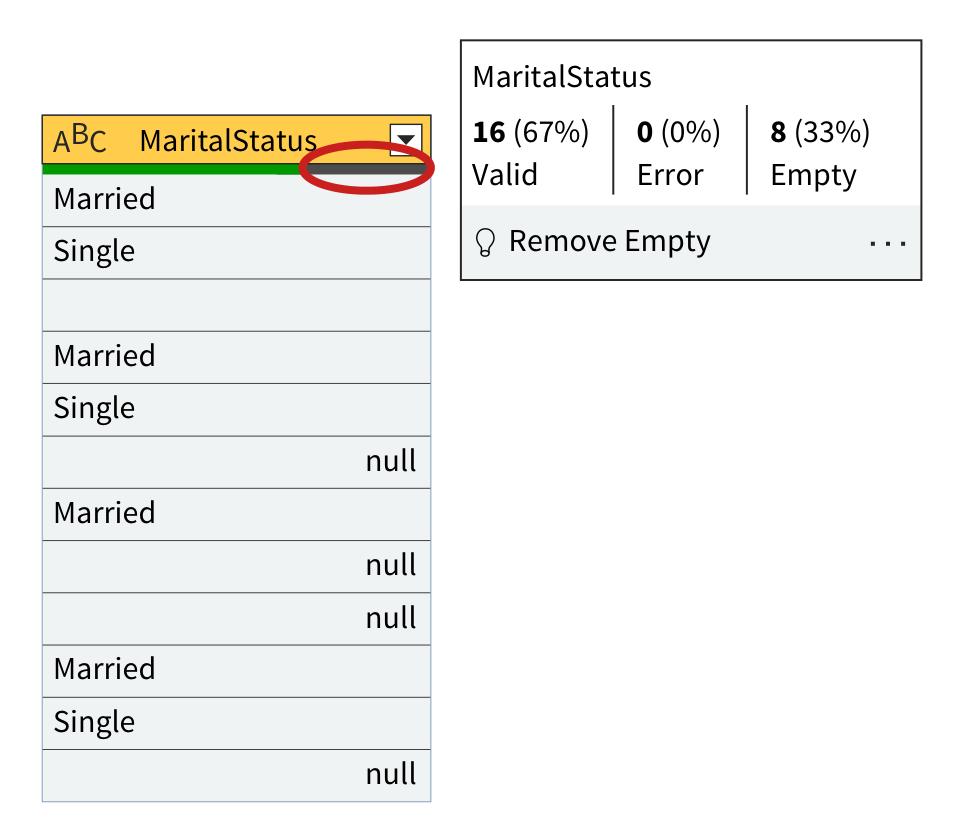
\includegraphics[width=0.95\textwidth,height=0.75\textheight,keepaspectratio]{../textbookForPractice/Figures/Ch_05/ILLUSTRATION 5.27.png}
    \end{figure}
\end{frame}

\begin{frame}{ILLUSTRATION 5.28}

    \begin{figure}[h]
        \centering
        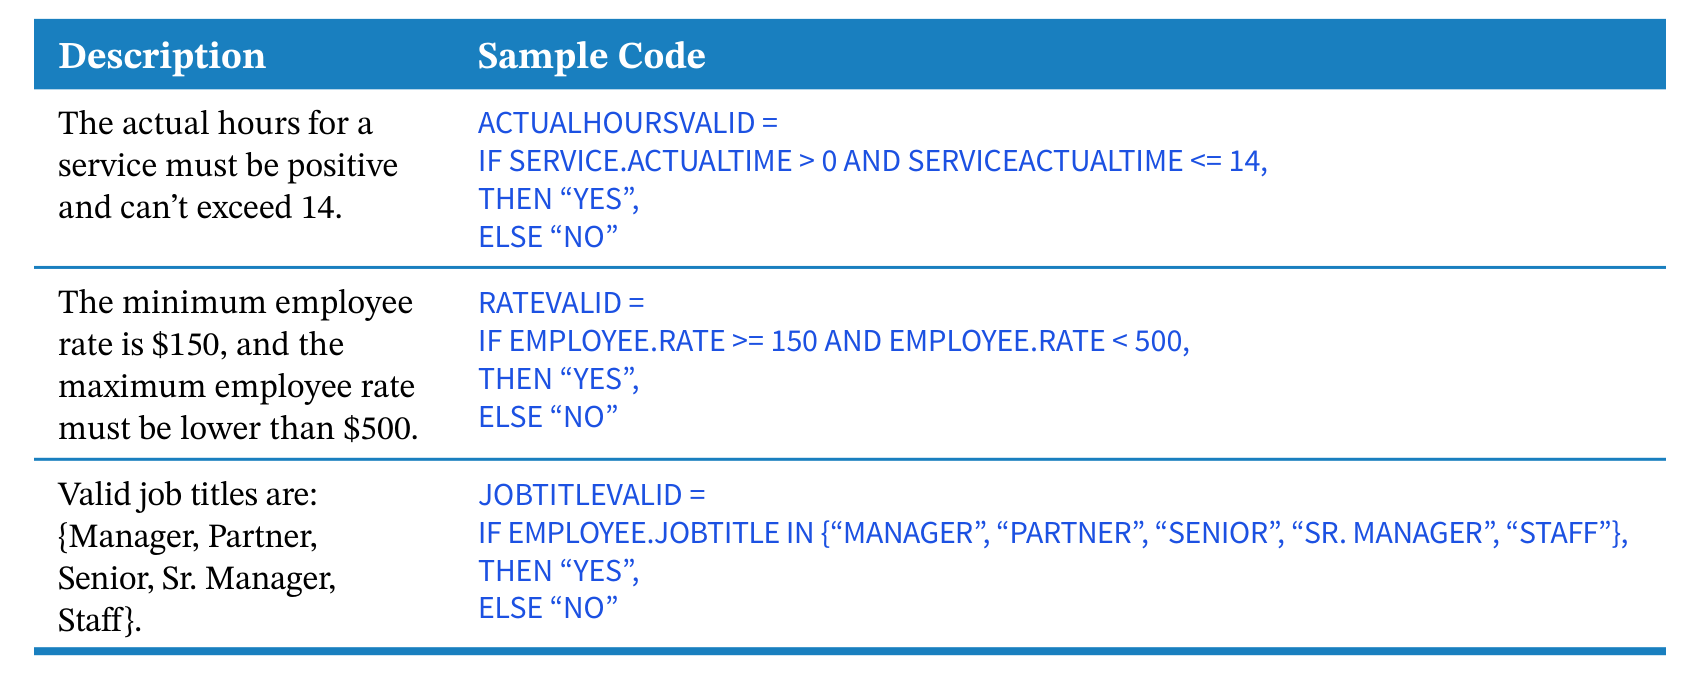
\includegraphics[width=0.95\textwidth,height=0.75\textheight,keepaspectratio]{../textbookForPractice/Figures/Ch_05/ILLUSTRATION 5.28.png}
    \end{figure}
\end{frame}

\begin{frame}{ILLUSTRATION 5.29}

    \begin{figure}[h]
        \centering
        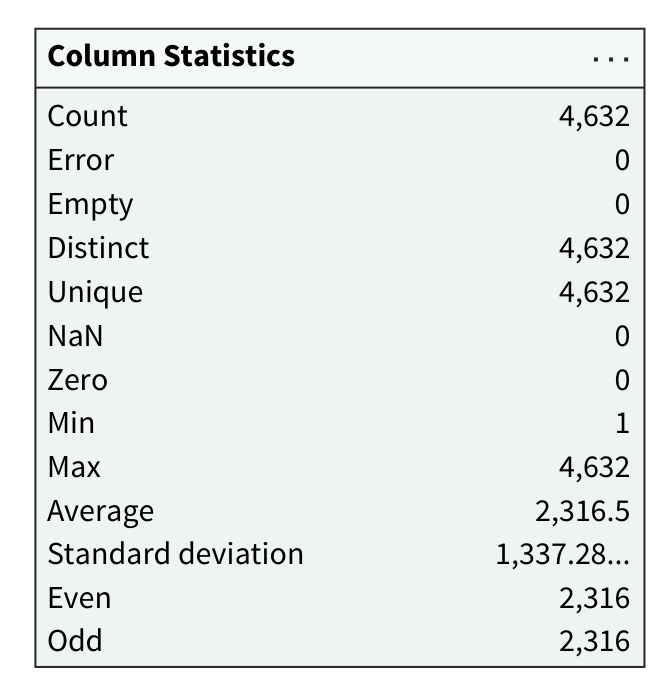
\includegraphics[width=0.95\textwidth,height=0.75\textheight,keepaspectratio]{../textbookForPractice/Figures/Ch_05/ILLUSTRATION 5.29.png}
    \end{figure}
\end{frame}

\begin{frame}{ILLUSTRATION 5.30}

    \begin{figure}[h]
        \centering
        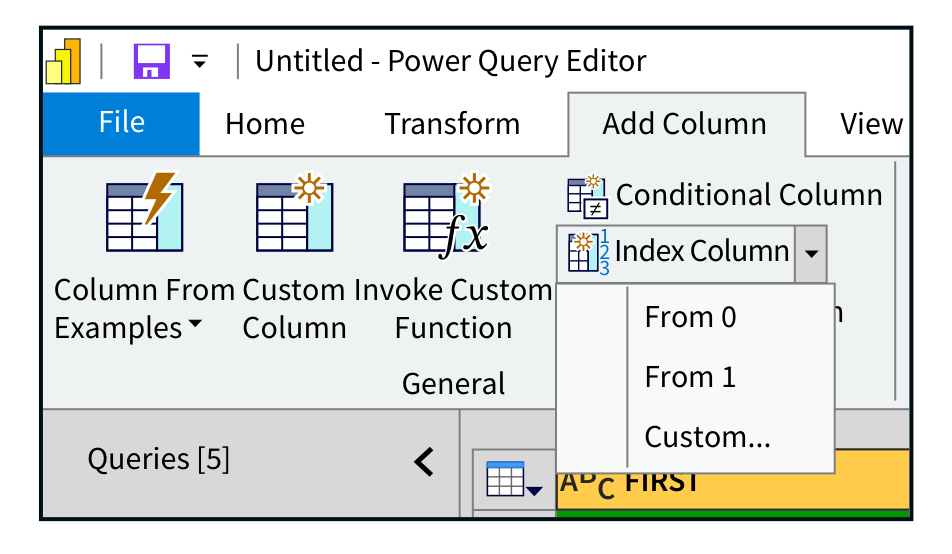
\includegraphics[width=0.95\textwidth,height=0.75\textheight,keepaspectratio]{../textbookForPractice/Figures/Ch_05/ILLUSTRATION 5.30.png}
    \end{figure}
\end{frame}

\begin{frame}{ILLUSTRATION 5.32}

    \begin{figure}[h]
        \centering
        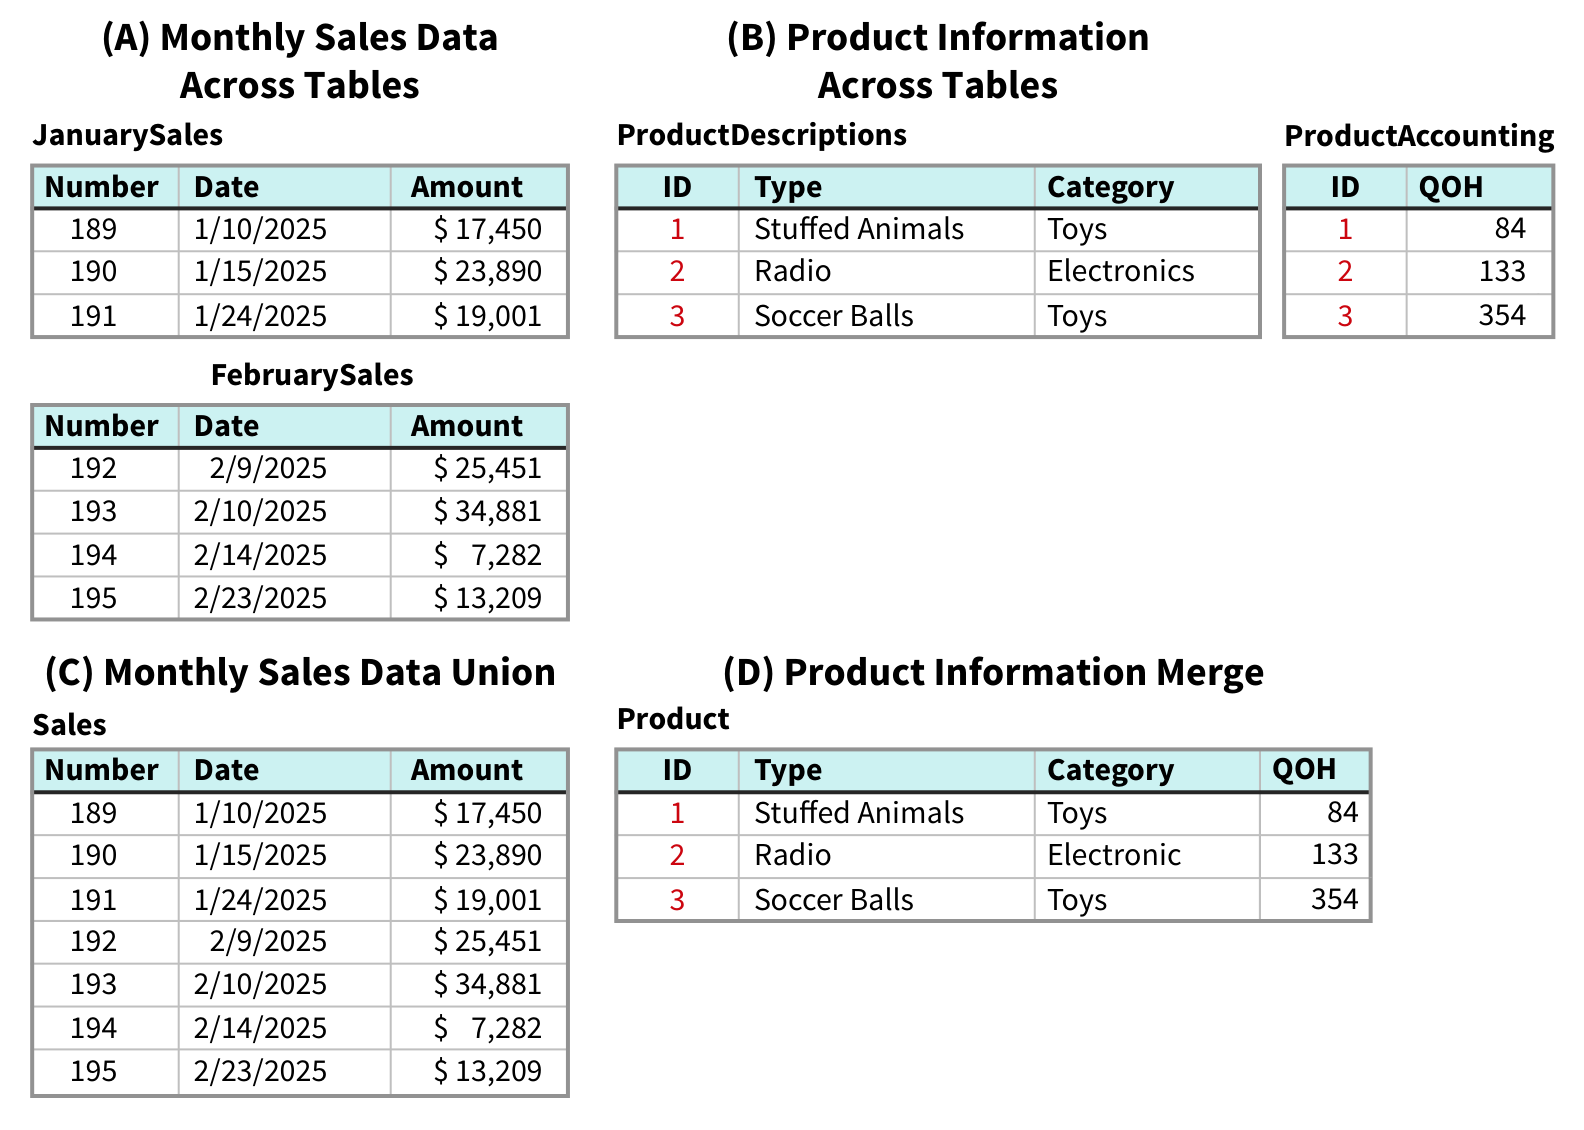
\includegraphics[width=0.95\textwidth,height=0.75\textheight,keepaspectratio]{../textbookForPractice/Figures/Ch_05/ILLUSTRATION 5.32.png}
    \end{figure}
\end{frame}

\begin{frame}{ILLUSTRATION 5.33}

    \begin{figure}[h]
        \centering
        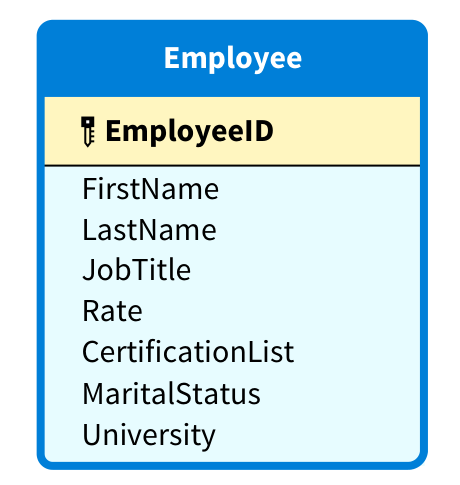
\includegraphics[width=0.95\textwidth,height=0.75\textheight,keepaspectratio]{../textbookForPractice/Figures/Ch_05/ILLUSTRATION 5.33.png}
    \end{figure}
\end{frame}

\begin{frame}{ILLUSTRATION 5.34}

    \begin{figure}[h]
        \centering
        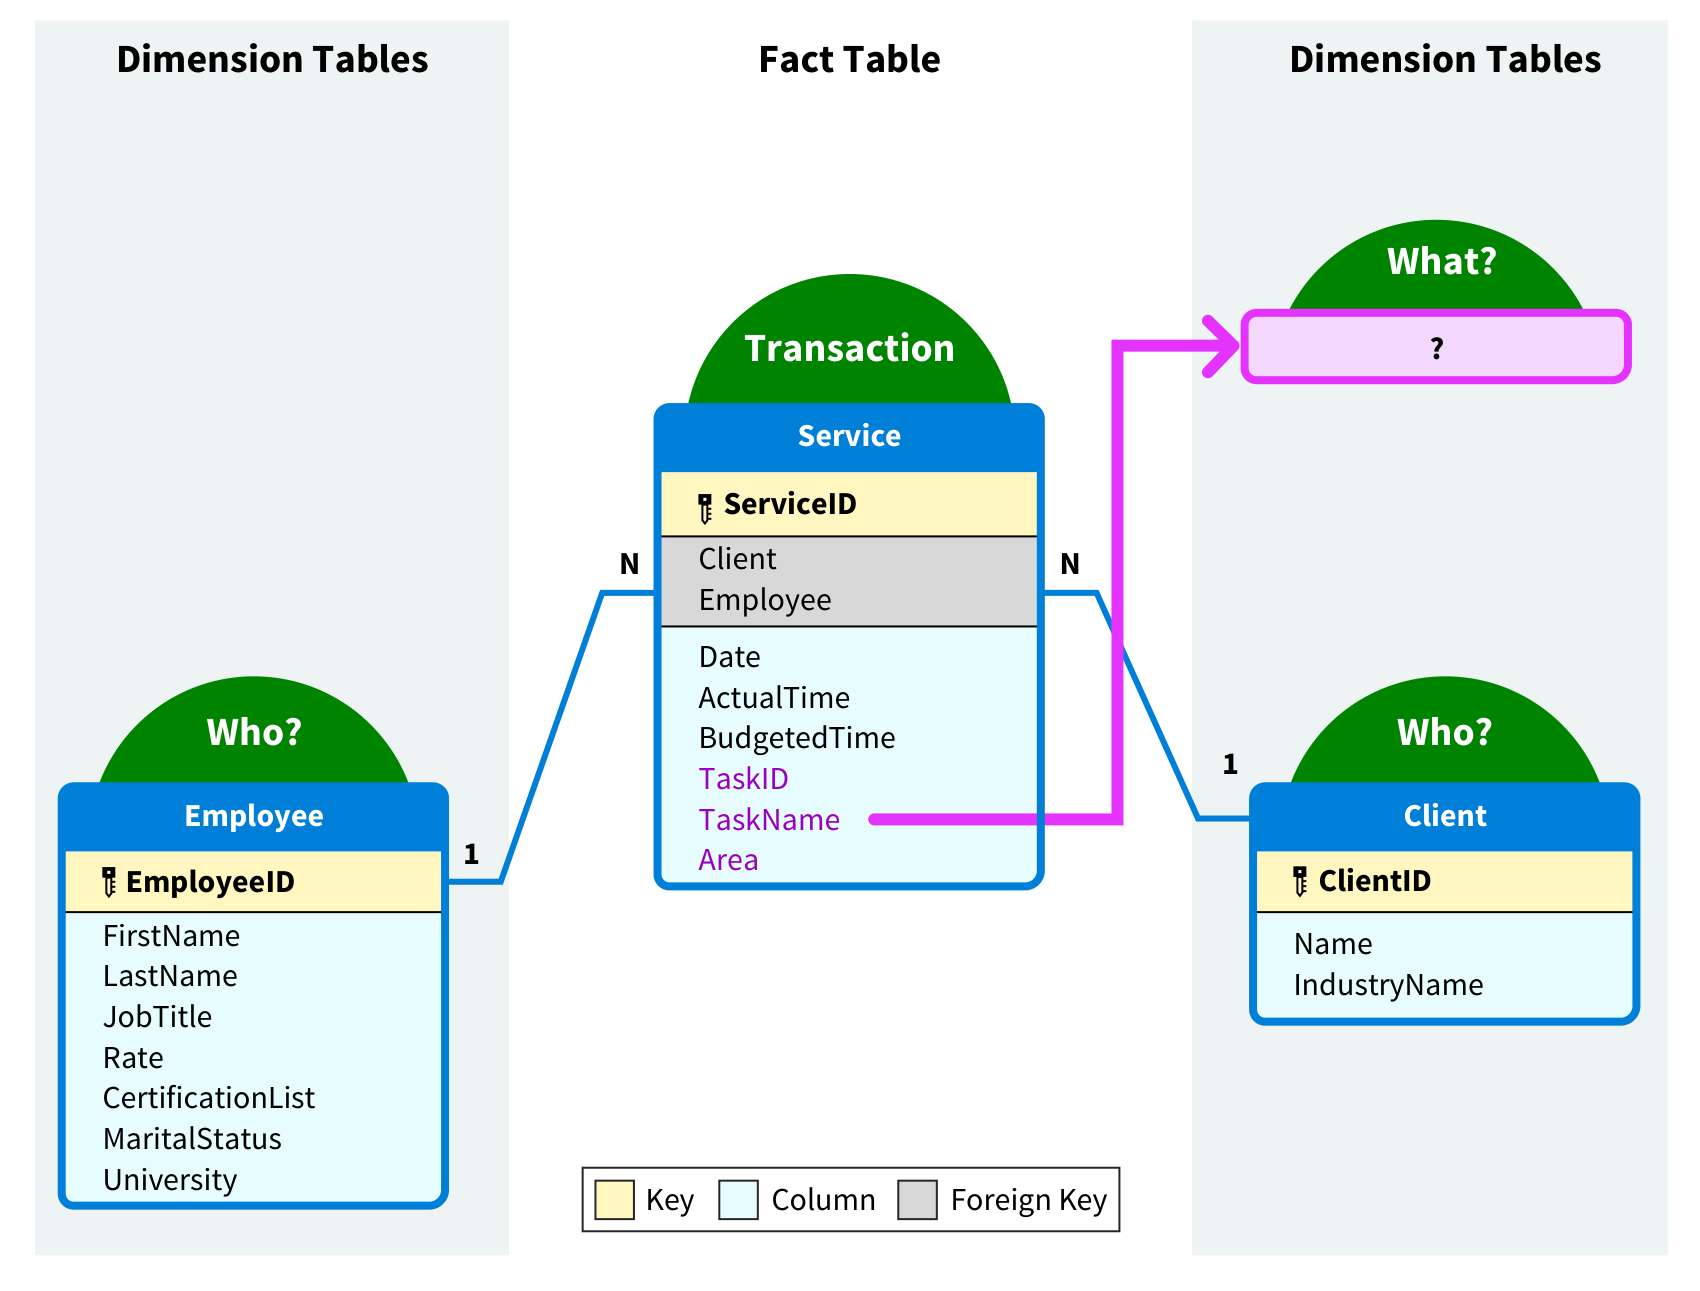
\includegraphics[width=0.95\textwidth,height=0.75\textheight,keepaspectratio]{../textbookForPractice/Figures/Ch_05/ILLUSTRATION 5.34.png}
    \end{figure}
\end{frame}

\begin{frame}{ILLUSTRATION 5.35}

    \begin{figure}[h]
        \centering
        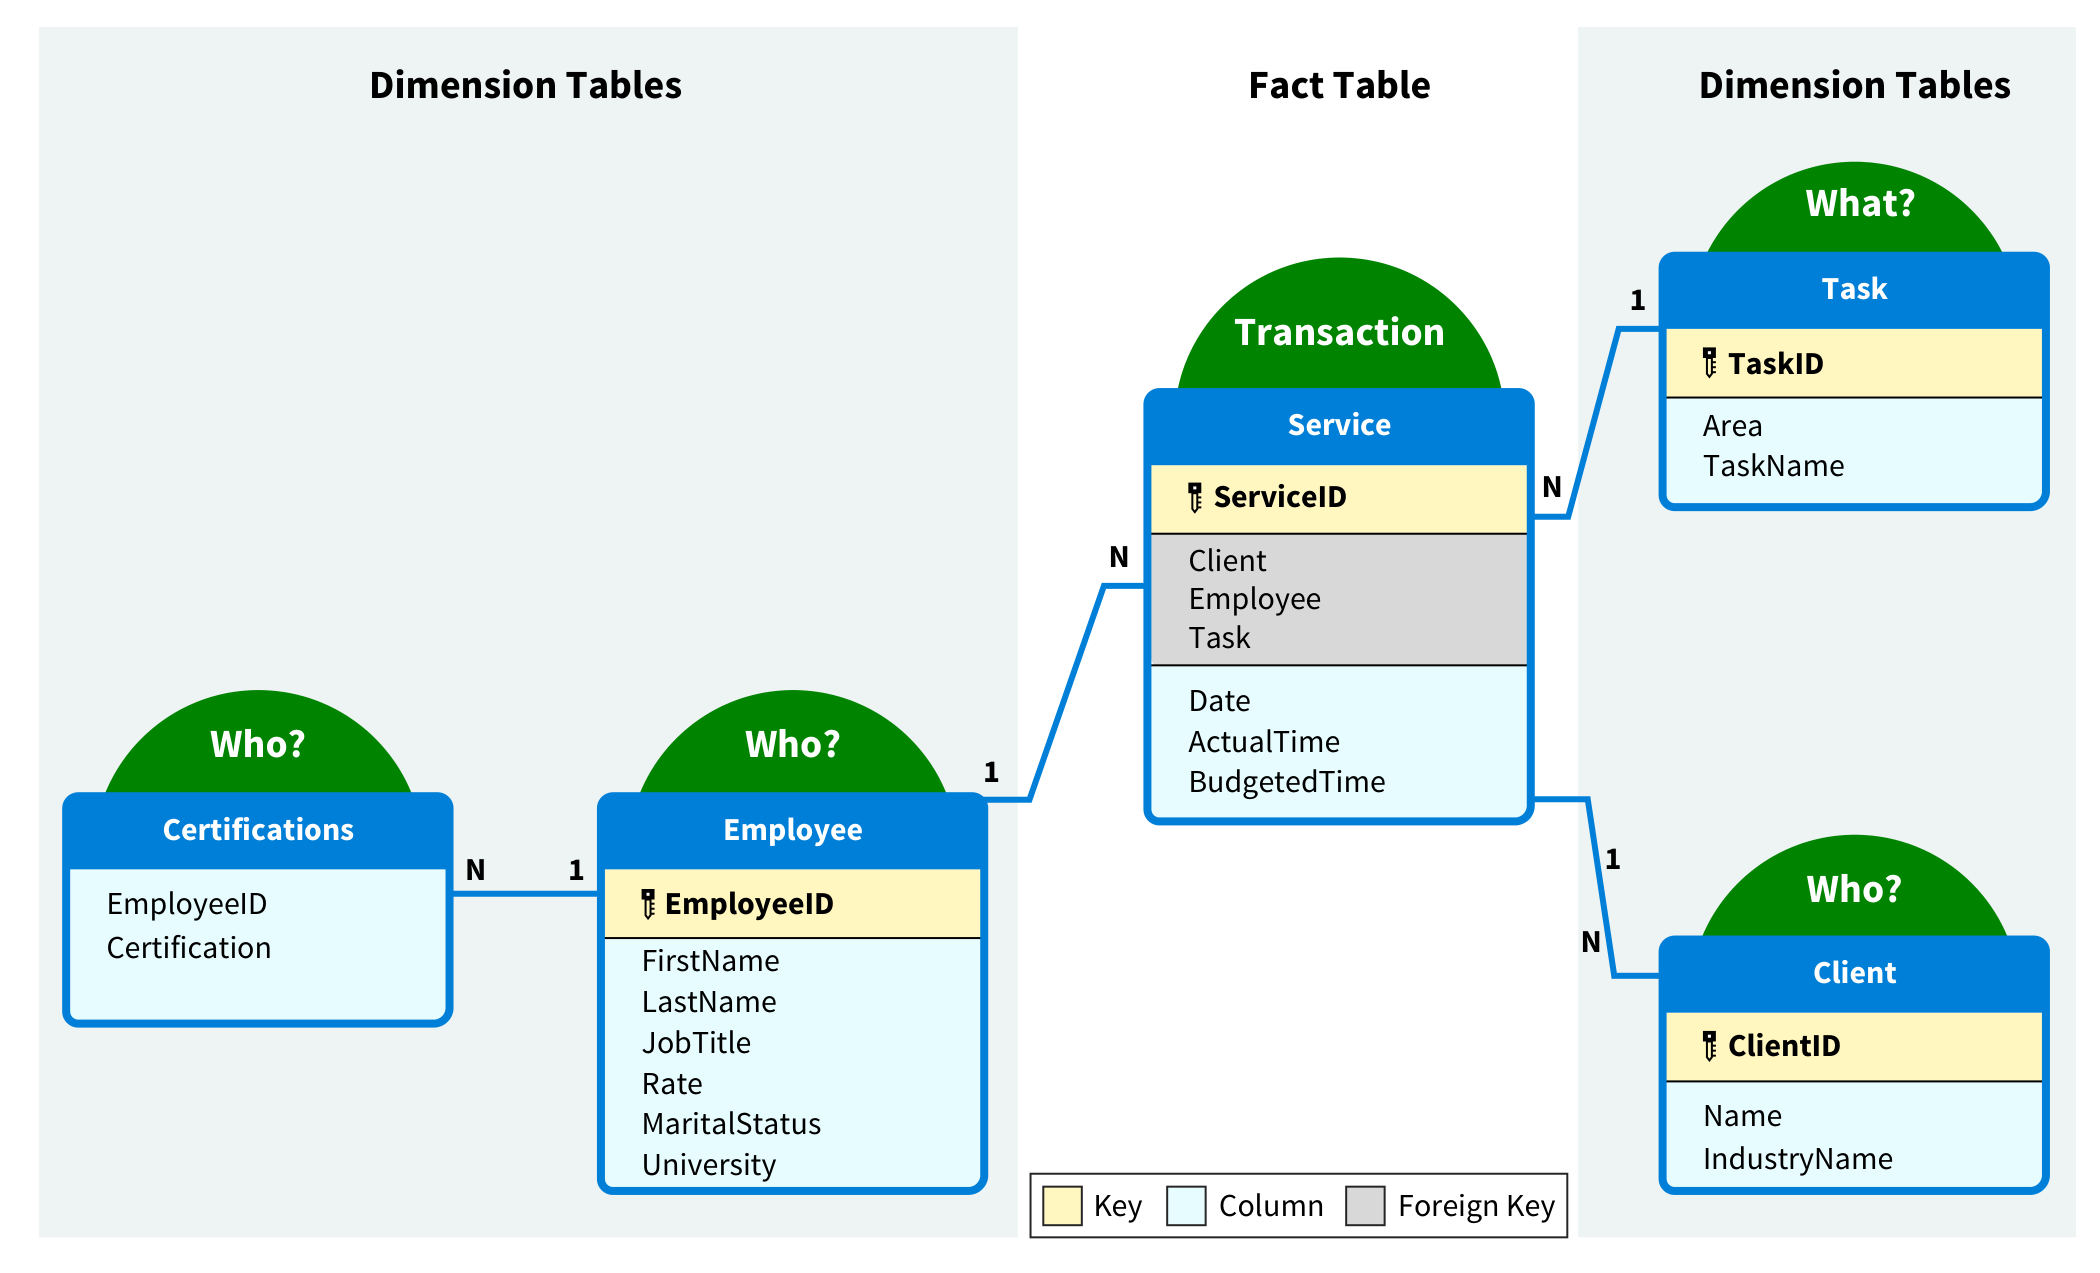
\includegraphics[width=0.95\textwidth,height=0.75\textheight,keepaspectratio]{../textbookForPractice/Figures/Ch_05/ILLUSTRATION 5.35.png}
    \end{figure}
\end{frame}

\begin{frame}{5.5 Áp dụng mẫu để Chuyển đổi Bảng (Table Transformation)}
\begin{itemize}
    \item \textbf{1. Lọc (Filtering):} Giữ lại các hàng thỏa mãn điều kiện (Ví dụ: Chỉ lấy doanh thu $> 1000$ USD).
    \item \textbf{2. Sắp xếp (Sorting):} Sắp xếp bảng theo thứ tự (Ví dụ: Bán chạy nhất lên đầu).
    \item \textbf{3. Gộp bảng theo cột (Join/Merge):} Kết hợp bảng "Hóa đơn" và "Khách hàng" dựa trên khóa chung (Mã KH).
    \item \textbf{4. Nối bảng theo hàng (Append/Union):} Nối dữ liệu bán hàng tháng 1 và tháng 2 vào chung một bảng (Phải có cùng số lượng cột và kiểu dữ liệu).
\end{itemize}
\end{frame}

\begin{frame}{ILLUSTRATION 5.36}

    \begin{figure}[h]
        \centering
        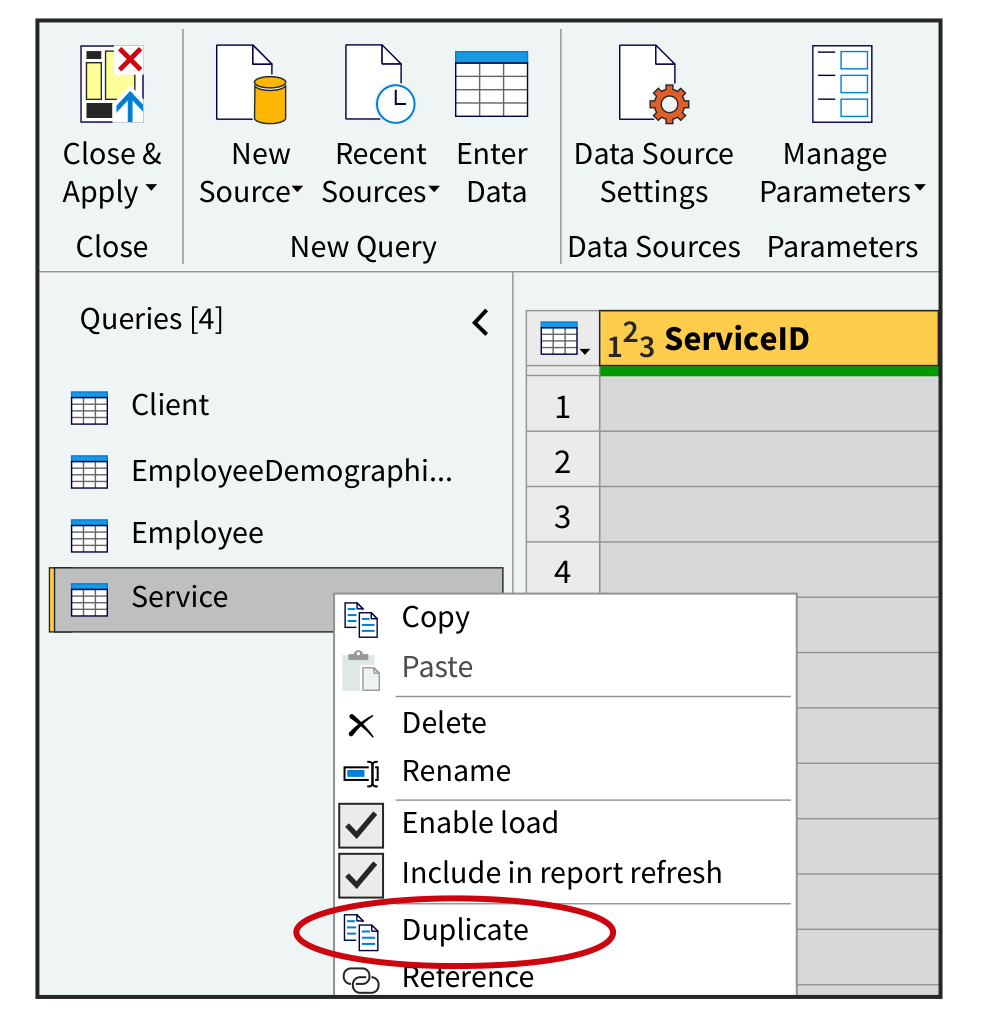
\includegraphics[width=0.95\textwidth,height=0.75\textheight,keepaspectratio]{../textbookForPractice/Figures/Ch_05/ILLUSTRATION 5.36.png}
    \end{figure}
\end{frame}

\begin{frame}{ILLUSTRATION 5.37}

    \begin{figure}[h]
        \centering
        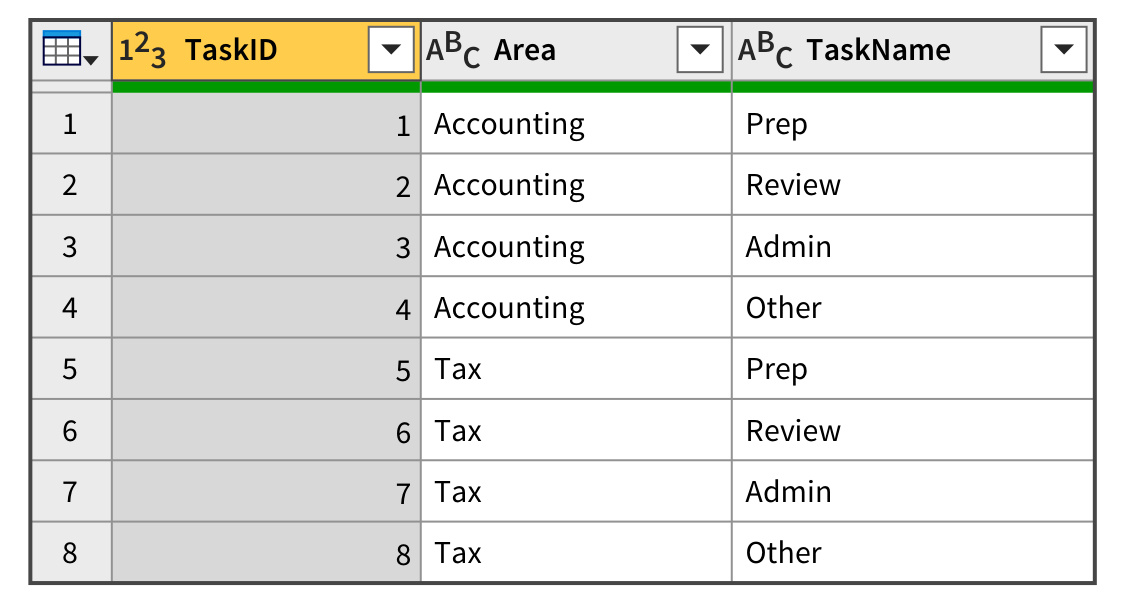
\includegraphics[width=0.95\textwidth,height=0.75\textheight,keepaspectratio]{../textbookForPractice/Figures/Ch_05/ILLUSTRATION 5.37.png}
    \end{figure}
\end{frame}

\begin{frame}{ILLUSTRATION 5.38}

    \begin{figure}[h]
        \centering
        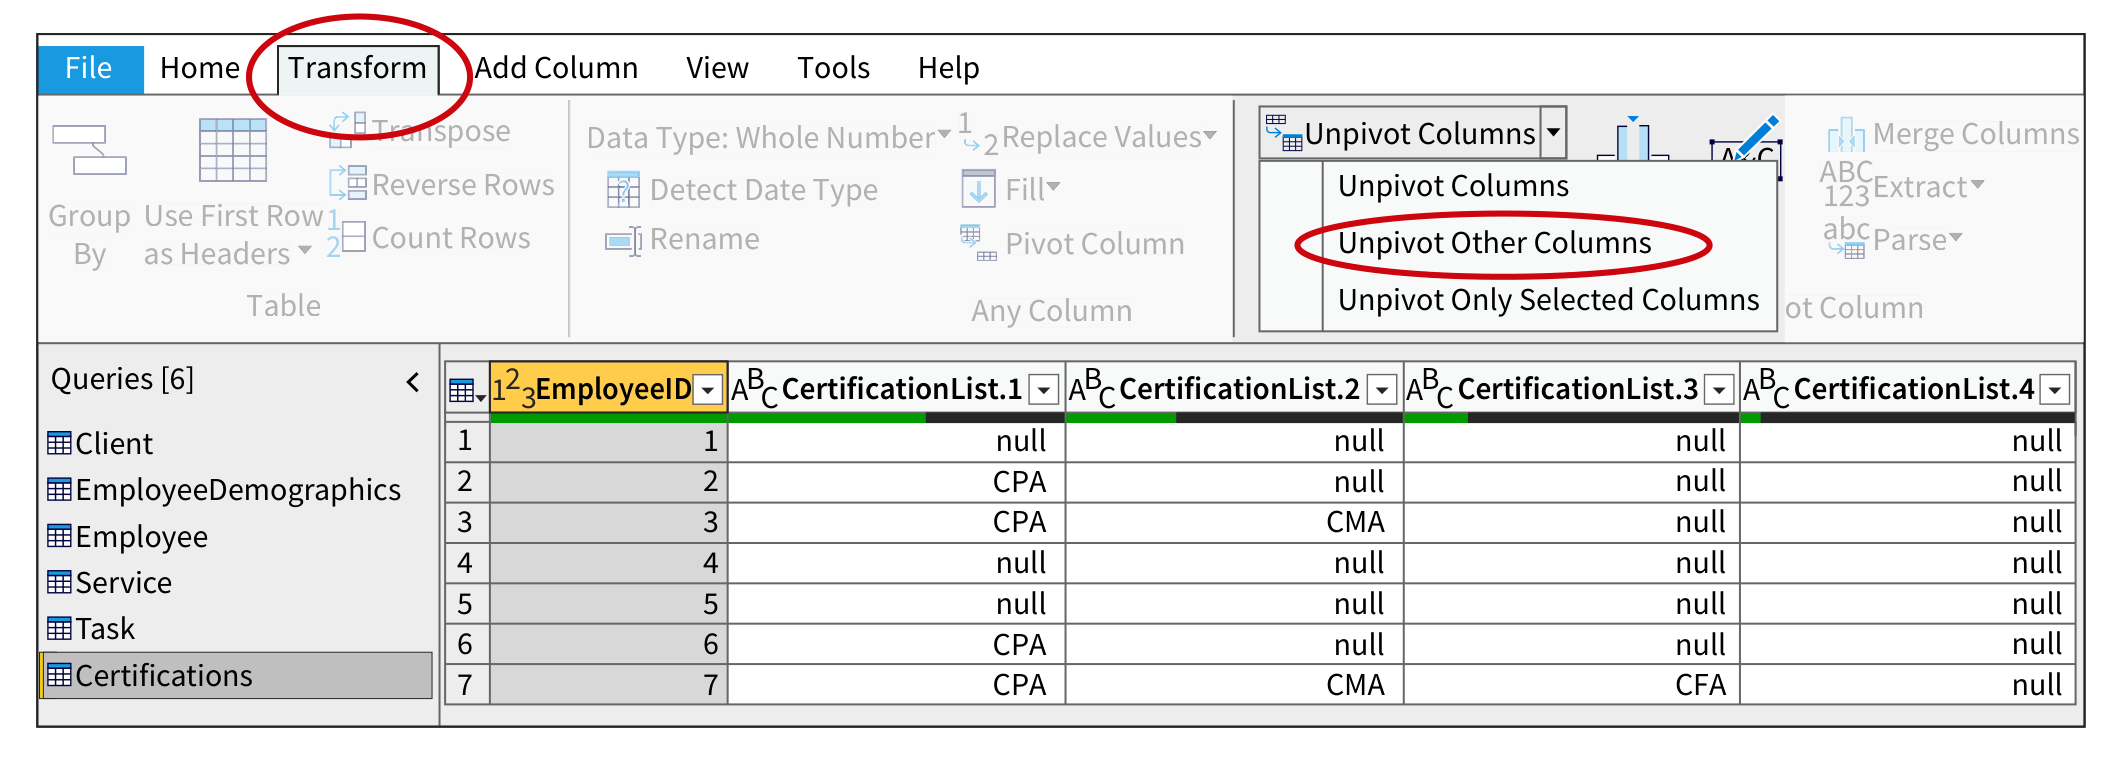
\includegraphics[width=0.95\textwidth,height=0.75\textheight,keepaspectratio]{../textbookForPractice/Figures/Ch_05/ILLUSTRATION 5.38.png}
    \end{figure}
\end{frame}

\begin{frame}{ILLUSTRATION 5.39}

    \begin{figure}[h]
        \centering
        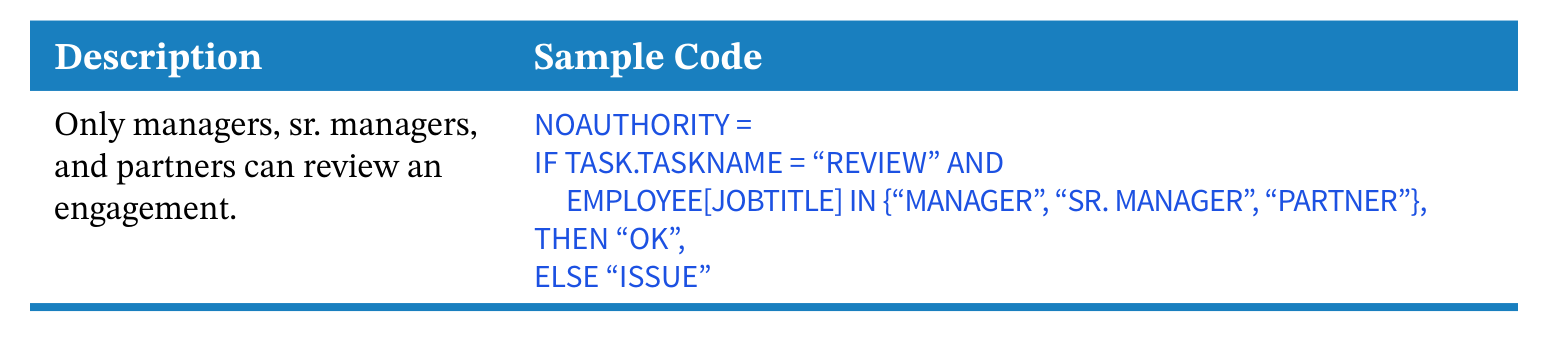
\includegraphics[width=0.95\textwidth,height=0.75\textheight,keepaspectratio]{../textbookForPractice/Figures/Ch_05/ILLUSTRATION 5.39.png}
    \end{figure}
\end{frame}

\begin{frame}{ILLUSTRATION 5.40}

    \begin{figure}[h]
        \centering
        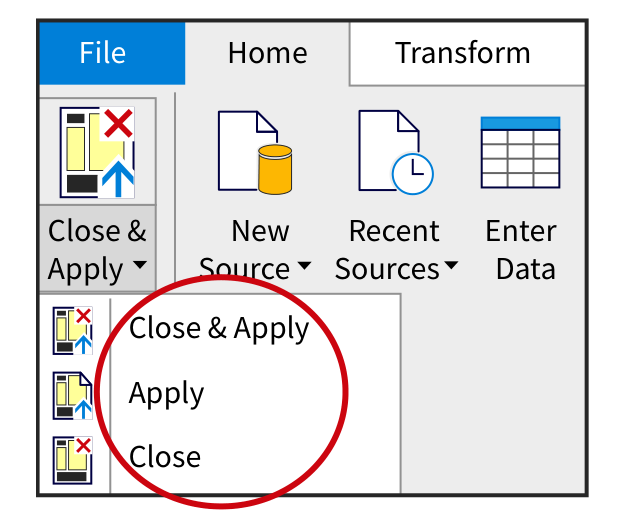
\includegraphics[width=0.95\textwidth,height=0.75\textheight,keepaspectratio]{../textbookForPractice/Figures/Ch_05/ILLUSTRATION 5.40.png}
    \end{figure}
\end{frame}

\begin{frame}{ILLUSTRATION 5.41}

    \begin{figure}[h]
        \centering
        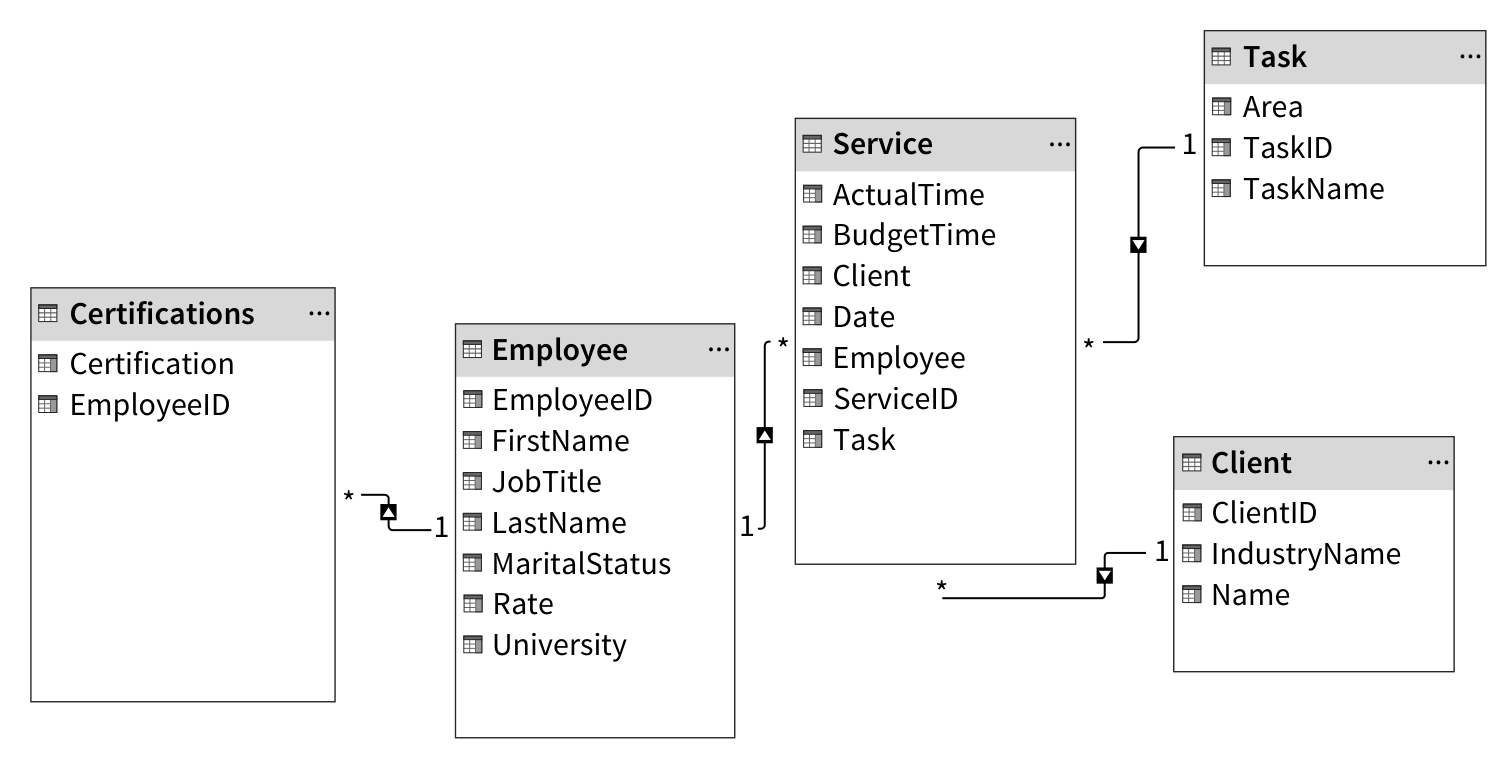
\includegraphics[width=0.95\textwidth,height=0.75\textheight,keepaspectratio]{../textbookForPractice/Figures/Ch_05/ILLUSTRATION 5.41.png}
    \end{figure}
\end{frame}

\begin{frame}{ILLUSTRATION 5.42}

    \begin{figure}[h]
        \centering
        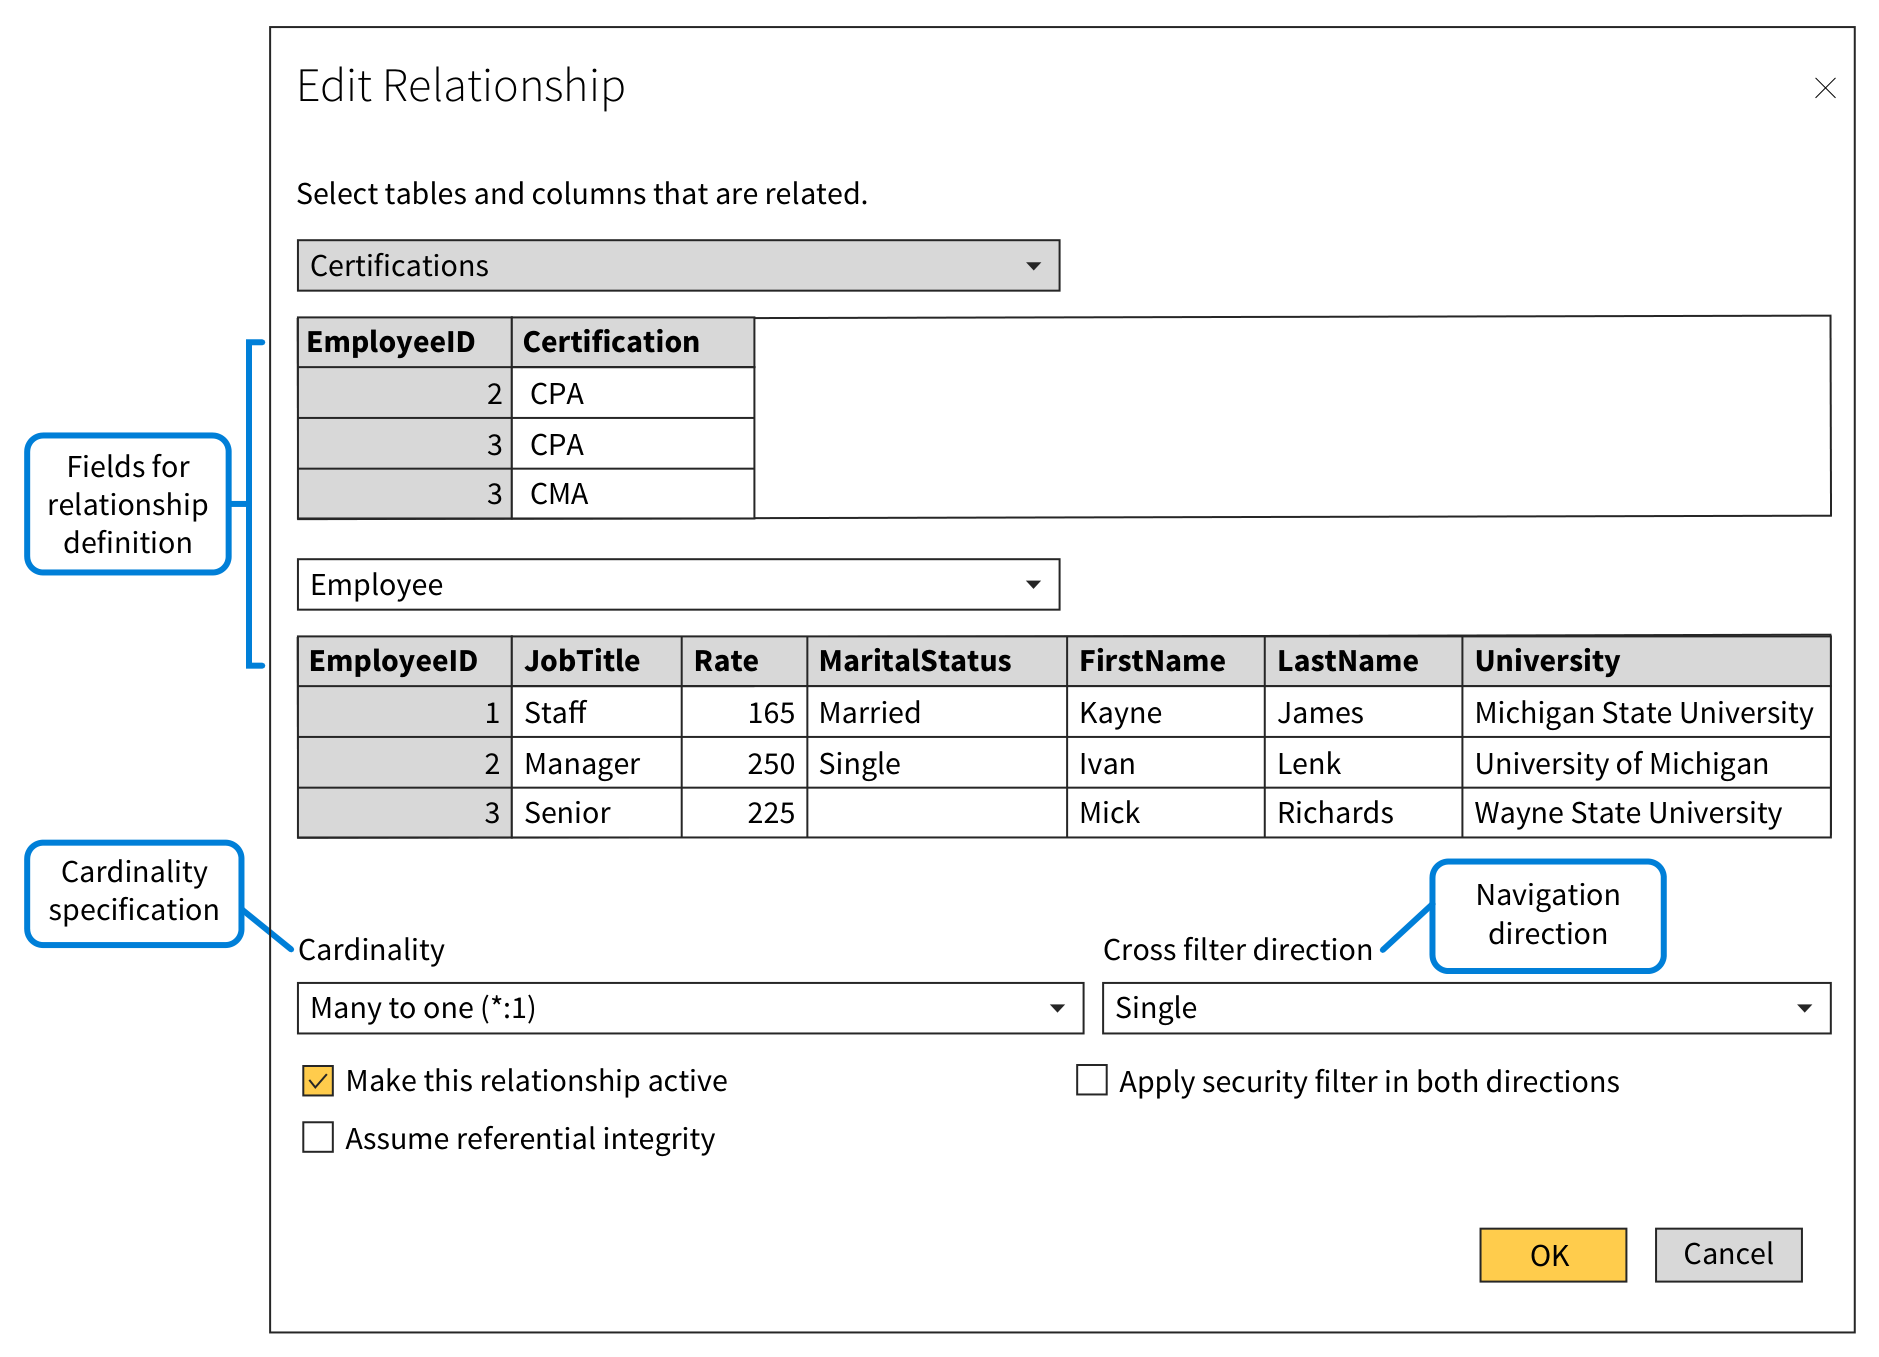
\includegraphics[width=0.95\textwidth,height=0.75\textheight,keepaspectratio]{../textbookForPractice/Figures/Ch_05/ILLUSTRATION 5.42.png}
    \end{figure}
\end{frame}

\begin{frame}{ILLUSTRATION 5.42\_1}

    \begin{figure}[h]
        \centering
        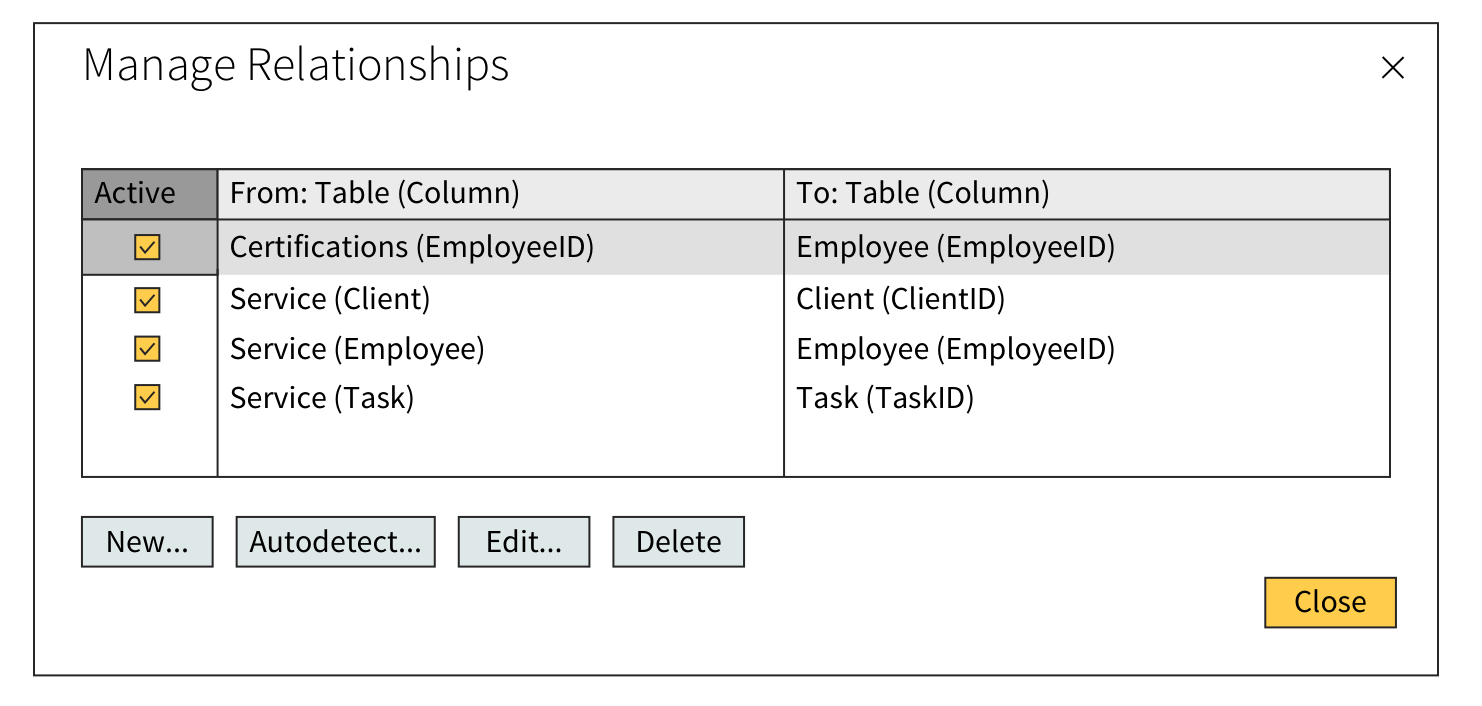
\includegraphics[width=0.95\textwidth,height=0.75\textheight,keepaspectratio]{../textbookForPractice/Figures/Ch_05/ILLUSTRATION 5.42_1.png}
    \end{figure}
\end{frame}

\begin{frame}{ILLUSTRATION 5.43}

    \begin{figure}[h]
        \centering
        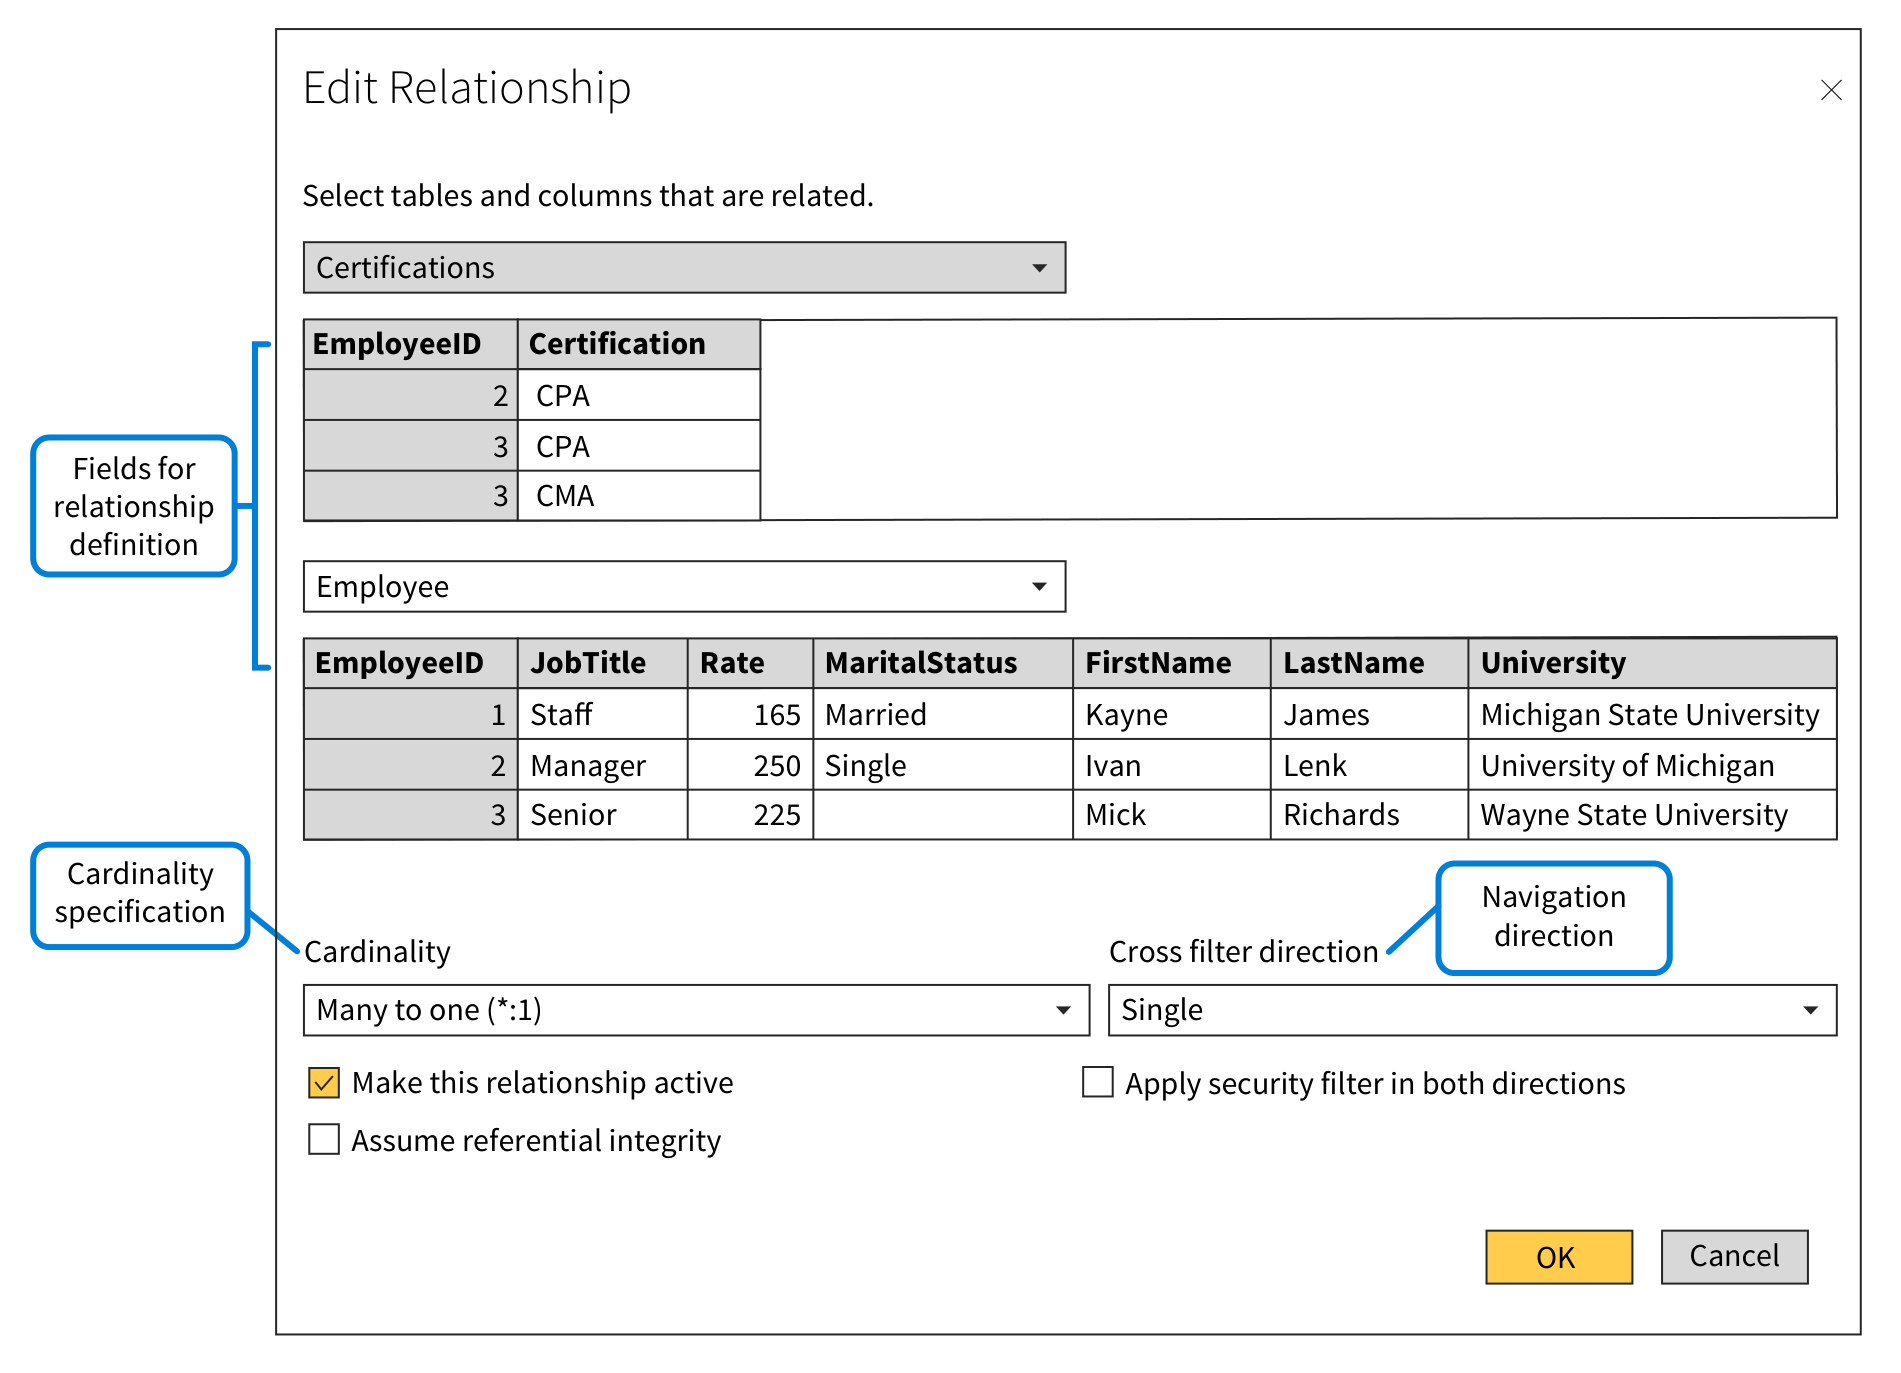
\includegraphics[width=0.95\textwidth,height=0.75\textheight,keepaspectratio]{../textbookForPractice/Figures/Ch_05/ILLUSTRATION 5.43.png}
    \end{figure}
\end{frame}

\begin{frame}{5.6 Áp dụng mẫu để Chuyển đổi Mô hình (Model Transformation)}
\begin{itemize}
    \item \textbf{Tổ chức Schema:} Từ nhiều bảng rời rạc, liên kết chúng lại thành một mô hình thống nhất để phân tích.
    \item \textbf{Star Schema (Mô hình Ngôi sao):} Gồm 1 Bảng Sự kiện (Fact Table) ở giữa chứa dữ liệu giao dịch, và các Bảng Danh mục (Dimension Tables) xung quanh. Tối ưu cho tốc độ truy vấn.
    \item \textbf{Snowflake Schema (Mô hình Bông tuyết):} Giống Star Schema nhưng các Bảng Danh mục được chuẩn hóa (chia nhỏ) tiếp. Tiết kiệm không gian lưu trữ nhưng làm chậm tốc độ phân tích.
\end{itemize}
\end{frame}

\begin{frame}{ILLUSTRATION 5.43\_1}

    \begin{figure}[h]
        \centering
        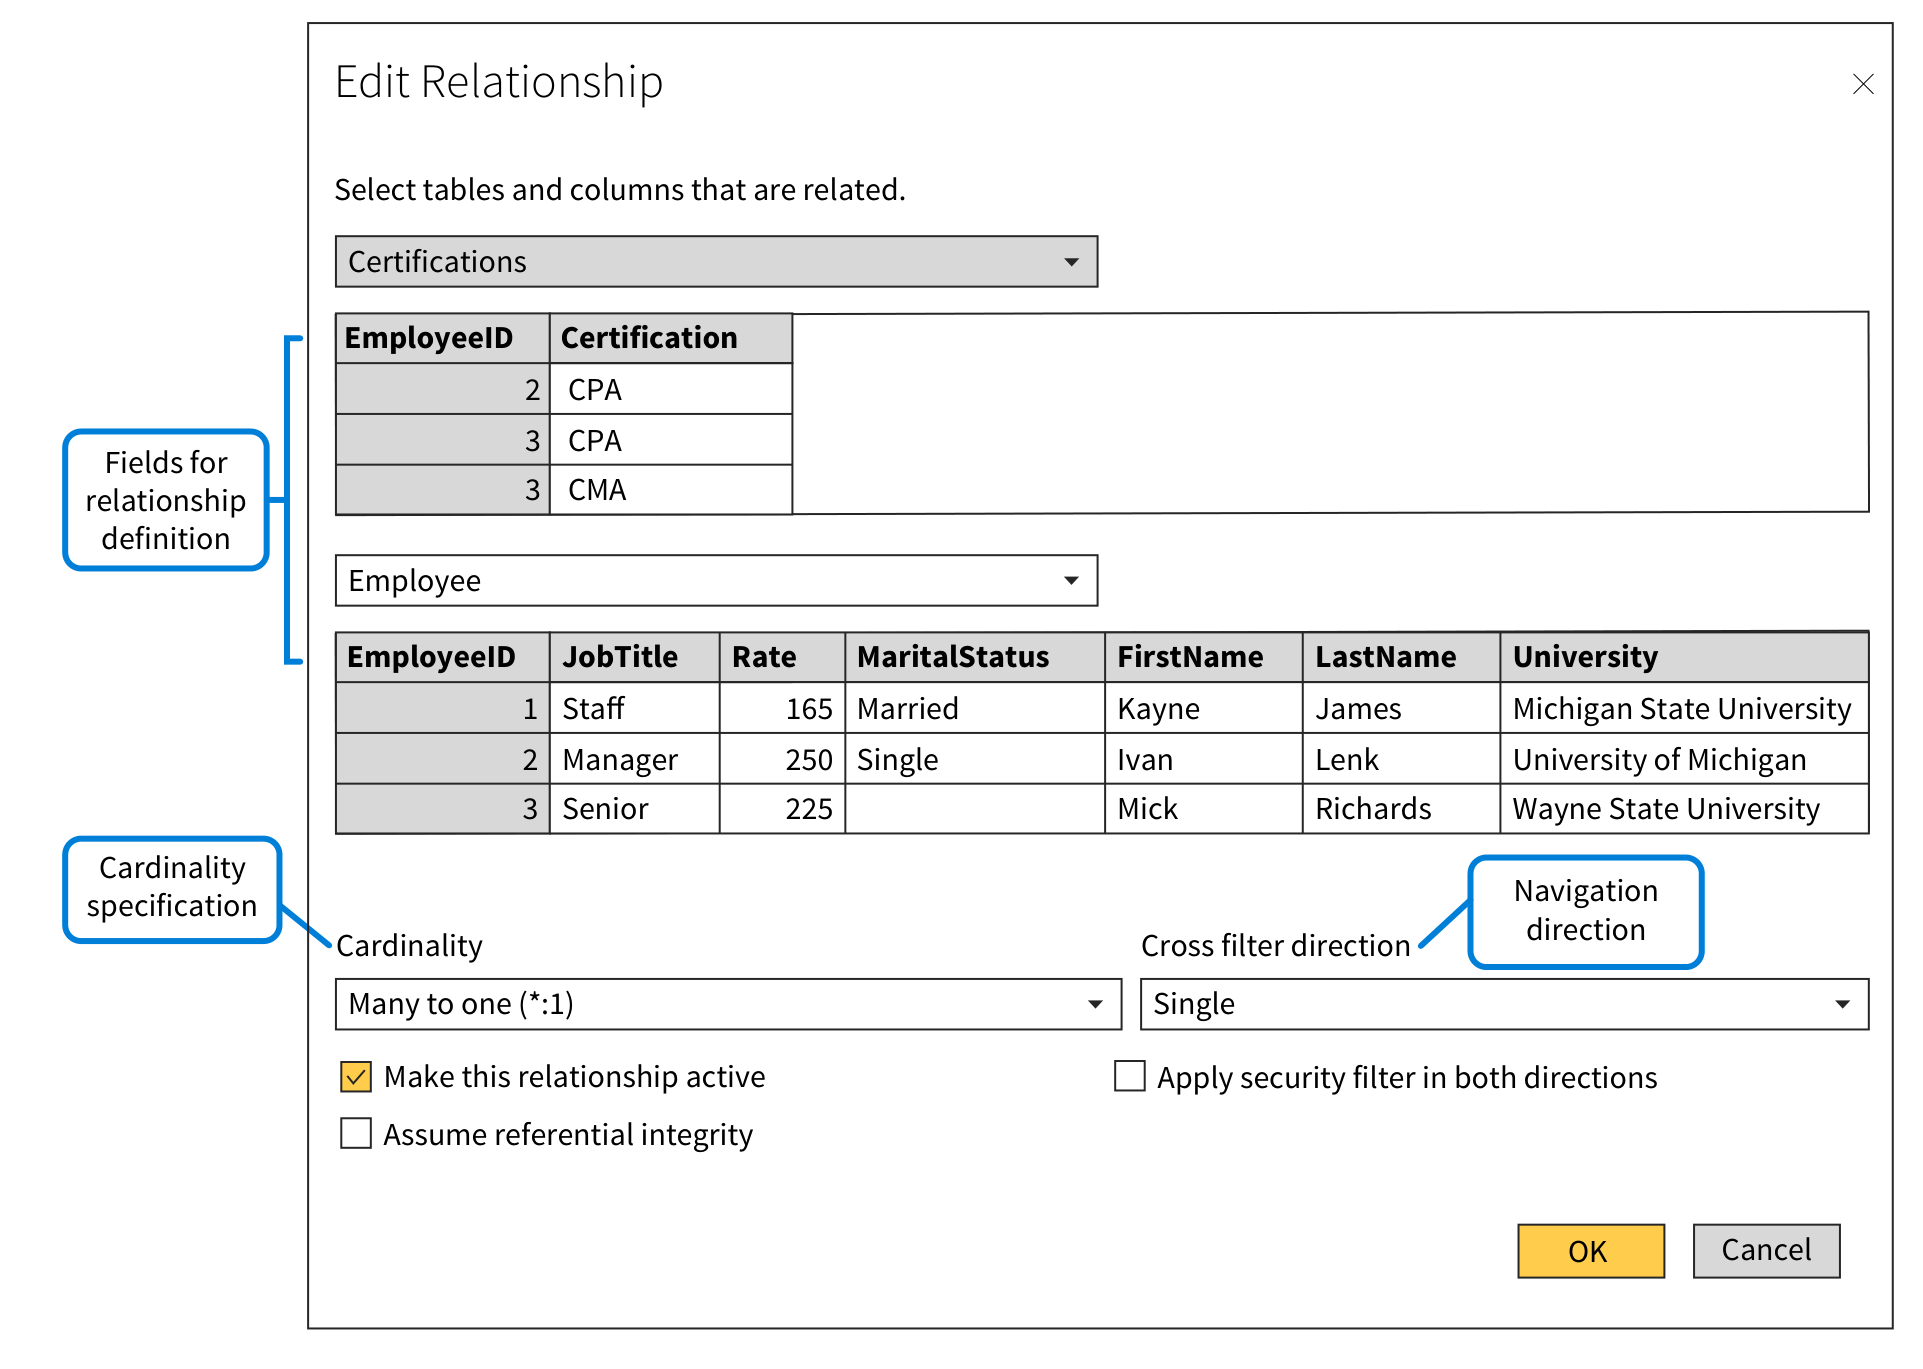
\includegraphics[width=0.95\textwidth,height=0.75\textheight,keepaspectratio]{../textbookForPractice/Figures/Ch_05/ILLUSTRATION 5.43_1.png}
    \end{figure}
\end{frame}

\begin{frame}{ILLUSTRATION 5.44}

    \begin{figure}[h]
        \centering
        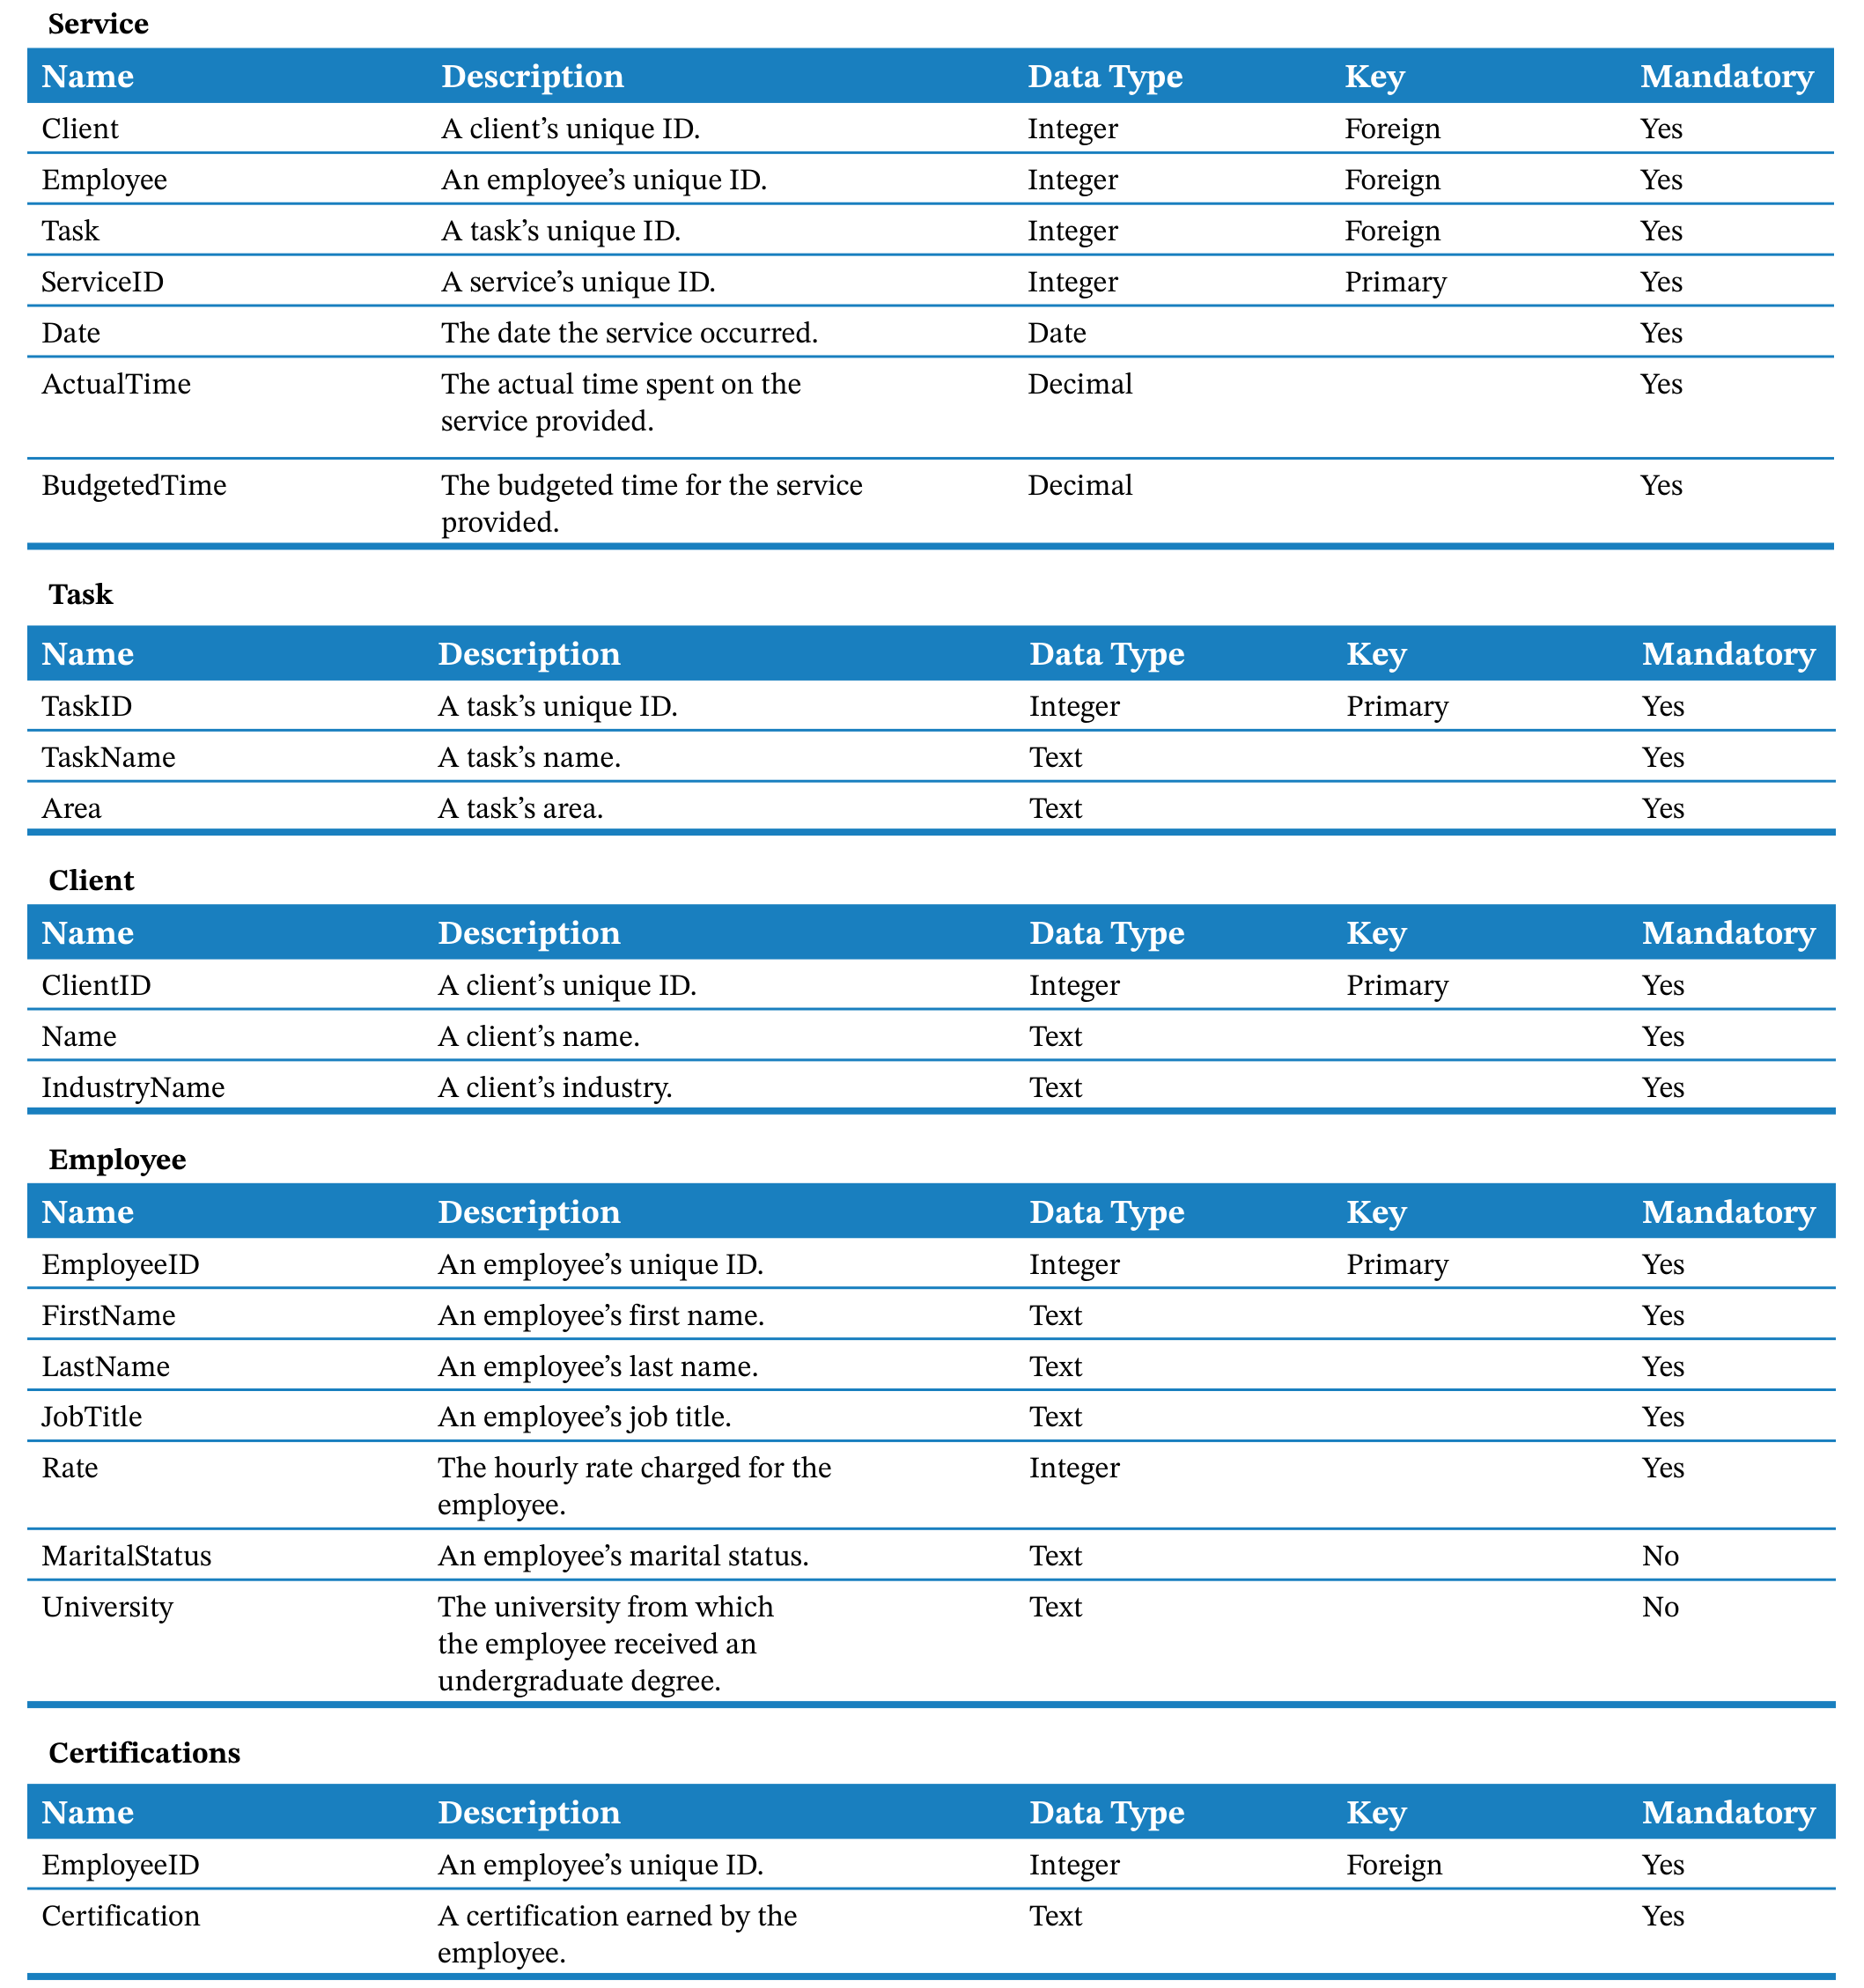
\includegraphics[width=0.95\textwidth,height=0.75\textheight,keepaspectratio]{../textbookForPractice/Figures/Ch_05/ILLUSTRATION 5.44.png}
    \end{figure}
\end{frame}

\begin{frame}{ILLUSTRATION 5.45}

    \begin{figure}[h]
        \centering
        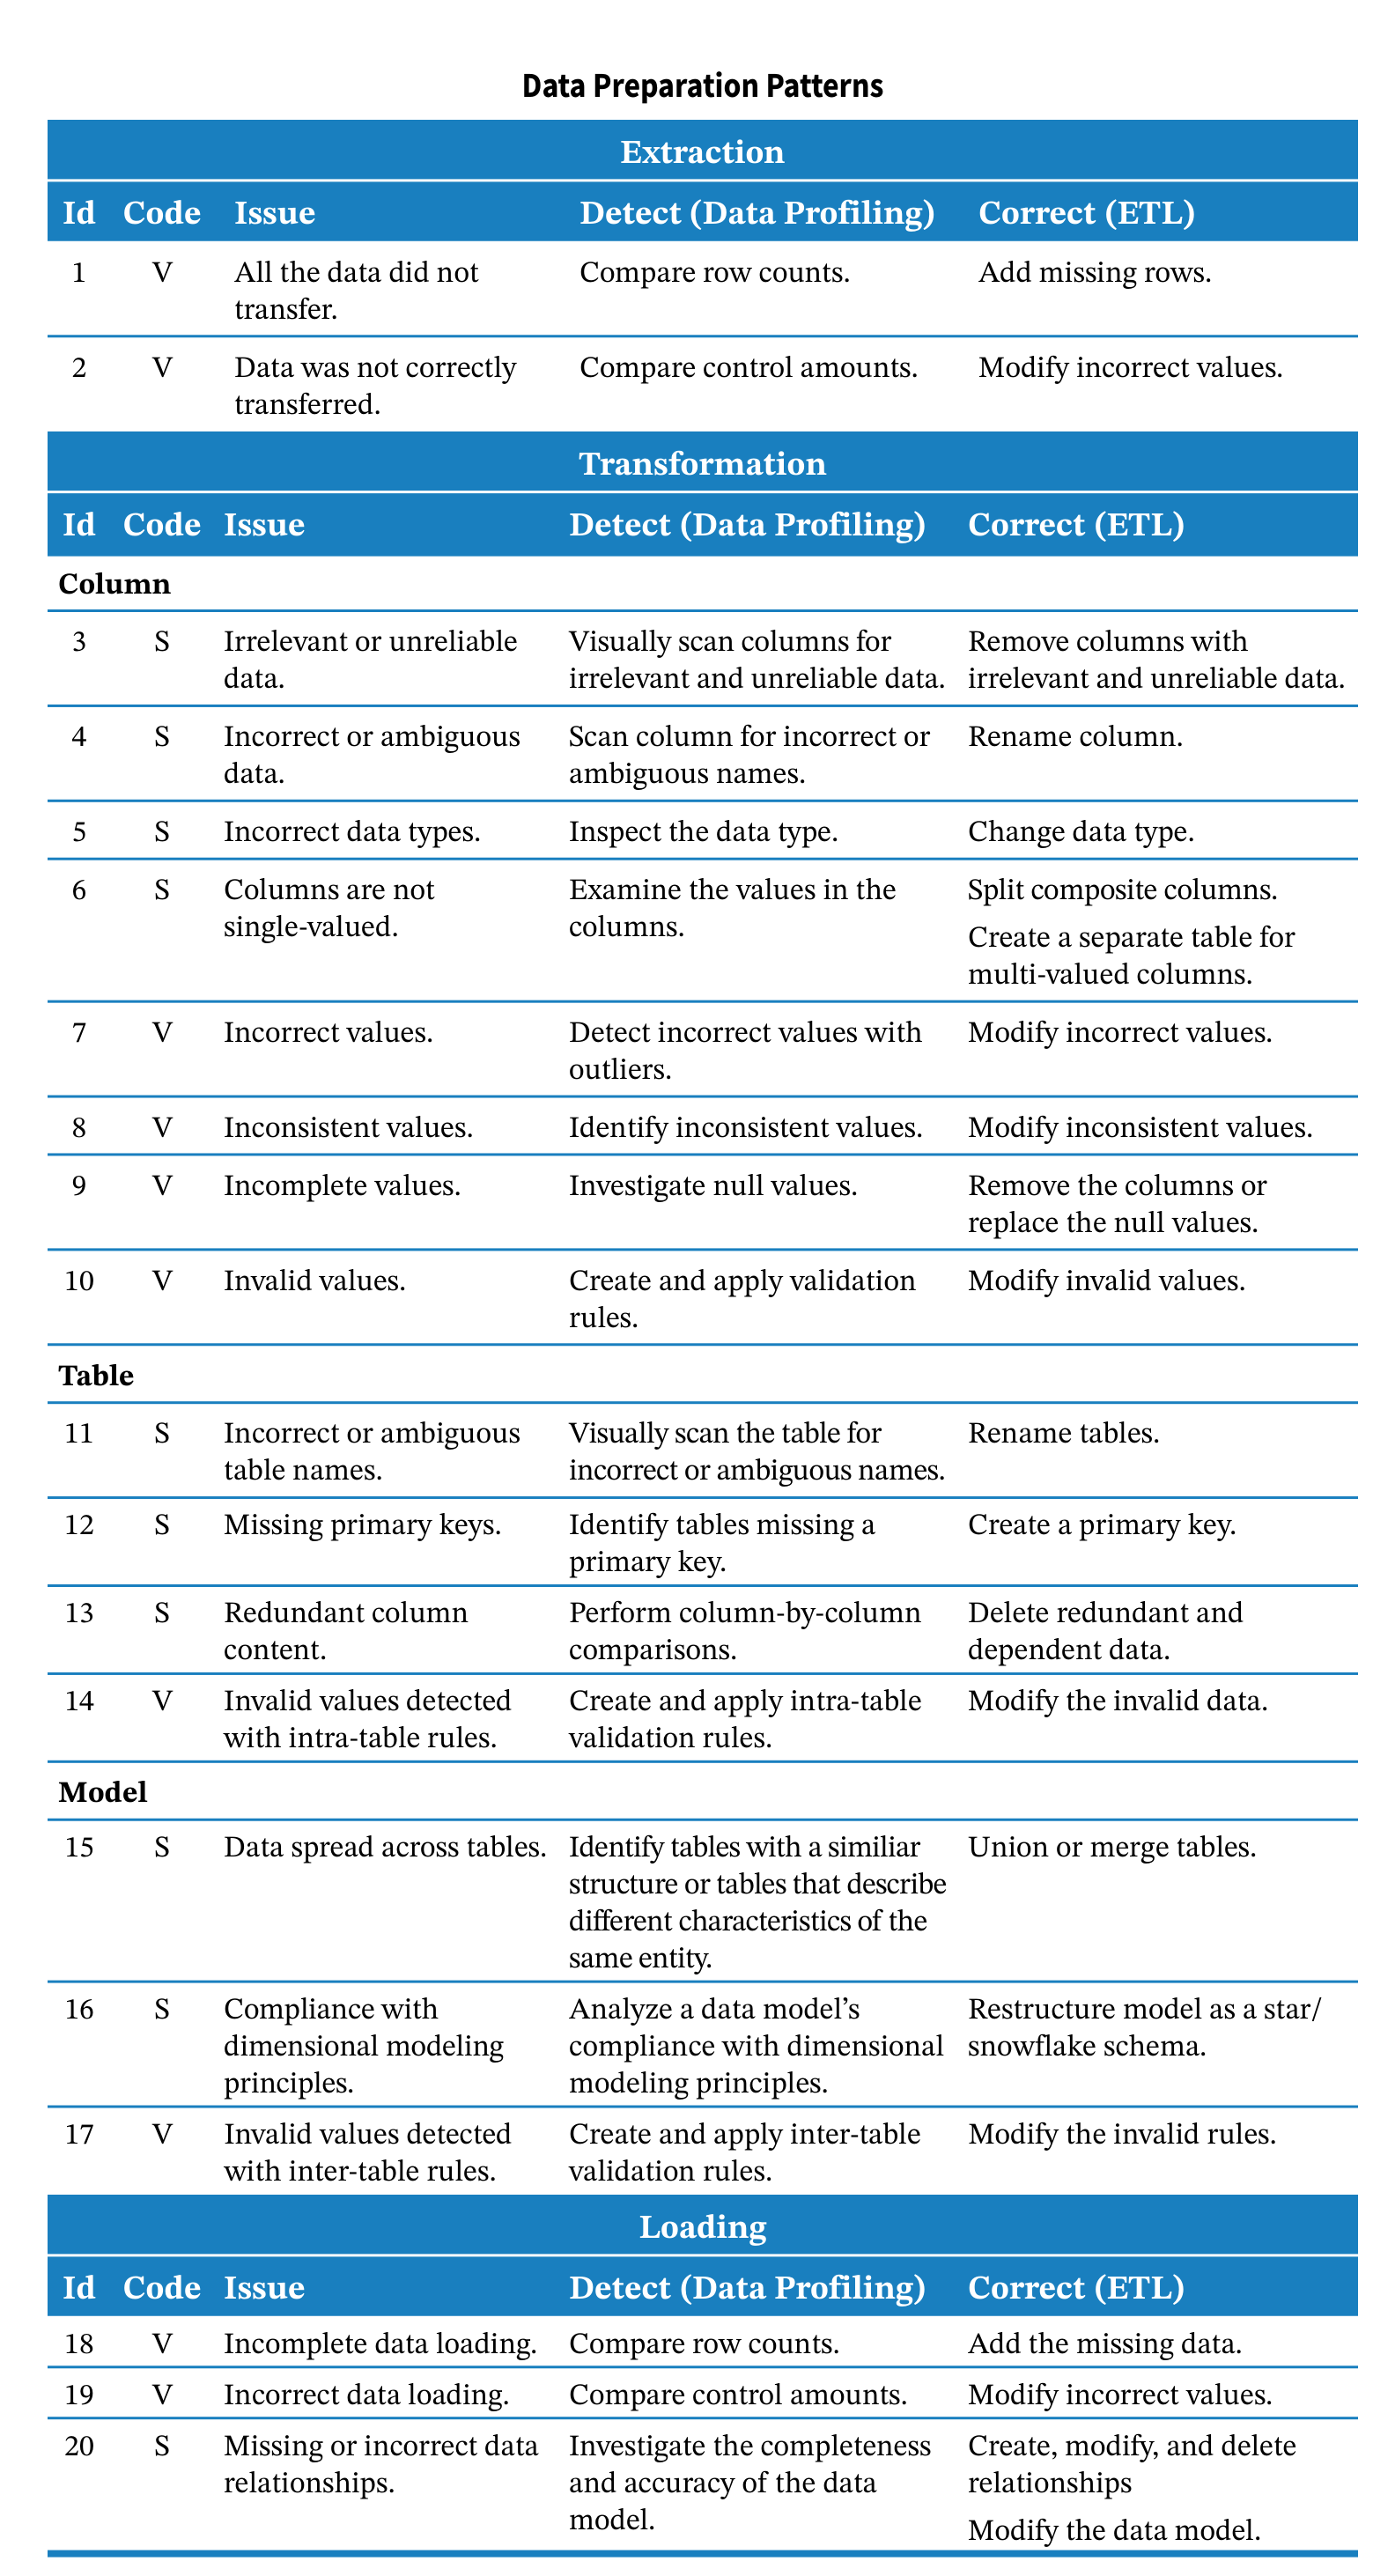
\includegraphics[width=0.95\textwidth,height=0.75\textheight,keepaspectratio]{../textbookForPractice/Figures/Ch_05/ILLUSTRATION 5.45.png}
    \end{figure}
\end{frame}

\begin{frame}{ILLUSTRATION 5.46}

    \begin{figure}[h]
        \centering
        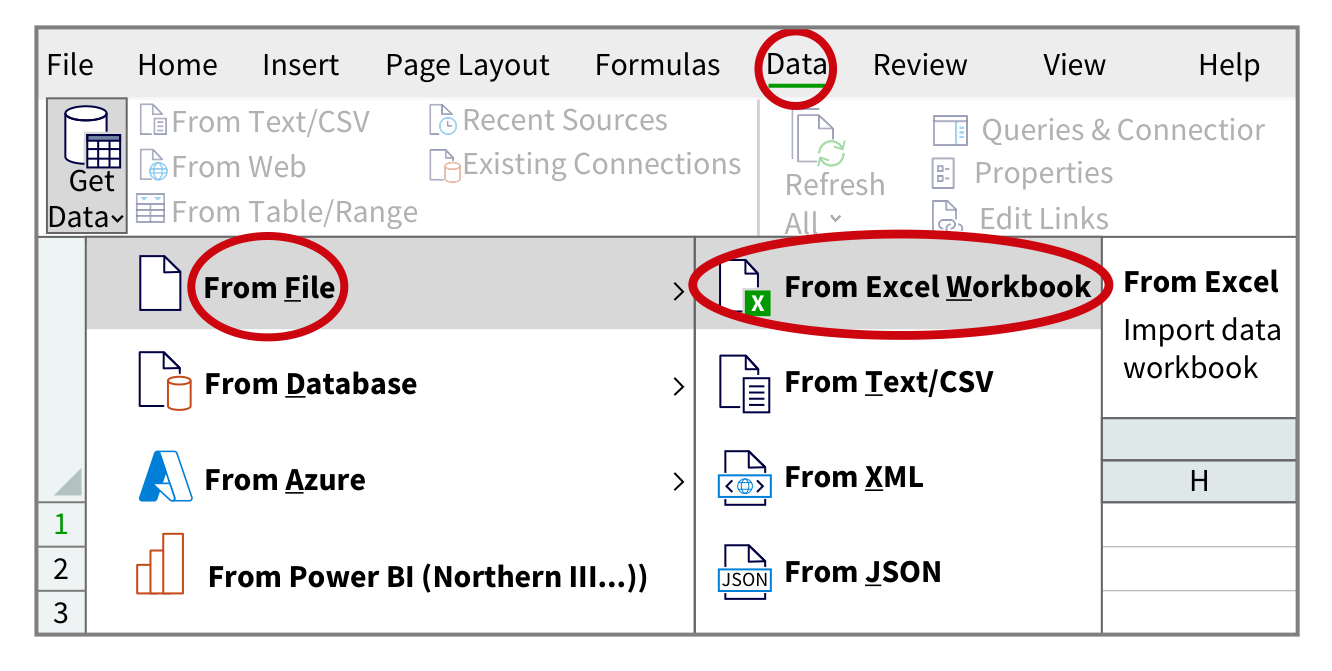
\includegraphics[width=0.95\textwidth,height=0.75\textheight,keepaspectratio]{../textbookForPractice/Figures/Ch_05/ILLUSTRATION 5.46.png}
    \end{figure}
\end{frame}

\begin{frame}{ILLUSTRATION 5.47}

    \begin{figure}[h]
        \centering
        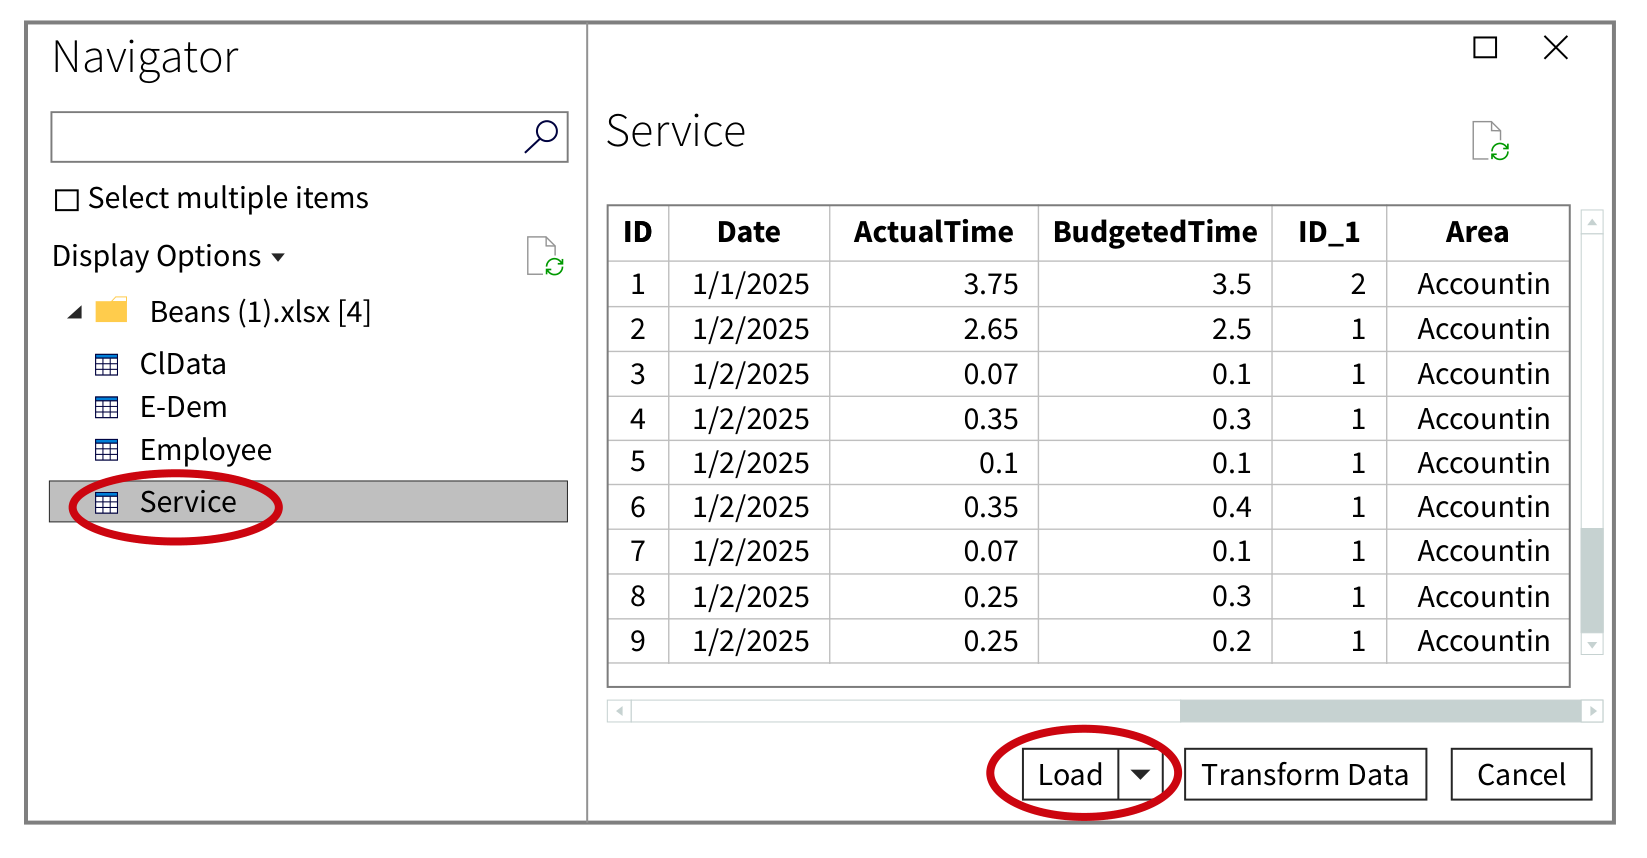
\includegraphics[width=0.95\textwidth,height=0.75\textheight,keepaspectratio]{../textbookForPractice/Figures/Ch_05/ILLUSTRATION 5.47.png}
    \end{figure}
\end{frame}

\begin{frame}{ILLUSTRATION 5.48}

    \begin{figure}[h]
        \centering
        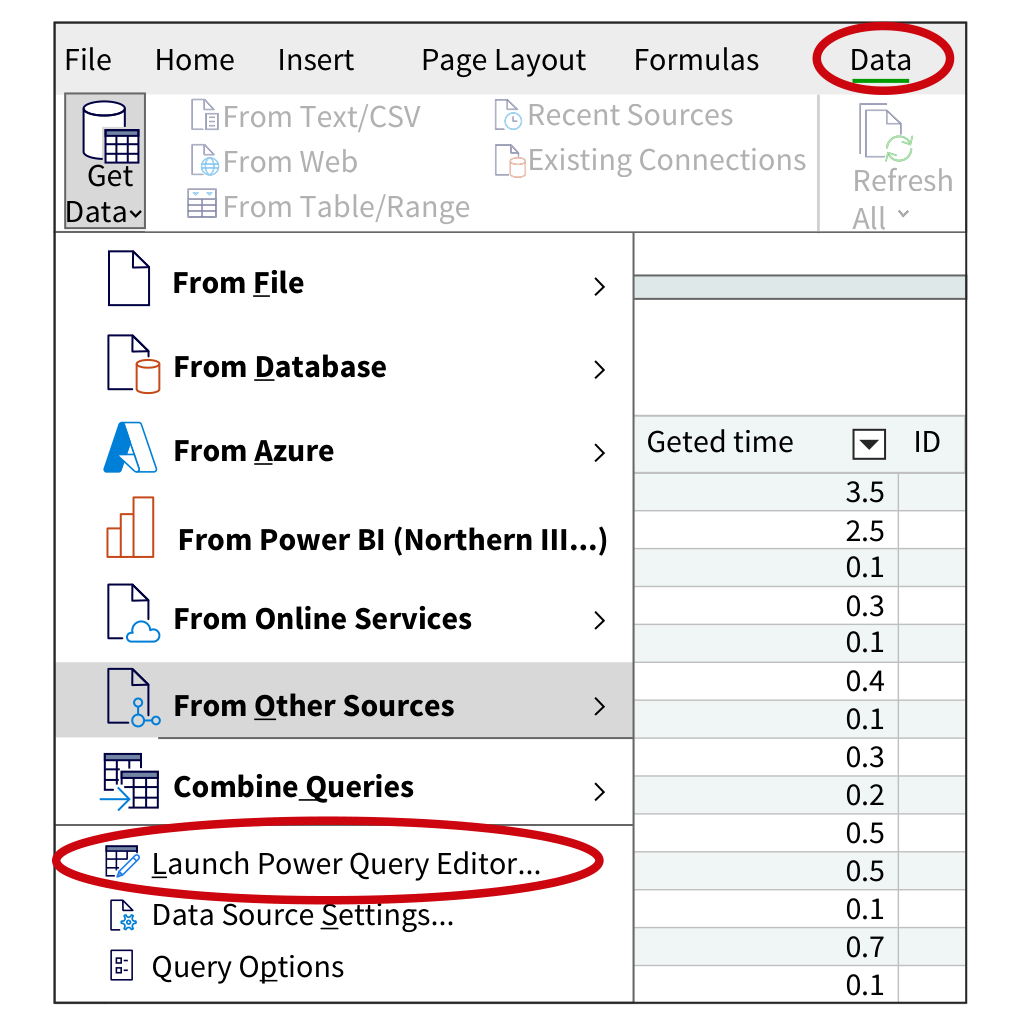
\includegraphics[width=0.95\textwidth,height=0.75\textheight,keepaspectratio]{../textbookForPractice/Figures/Ch_05/ILLUSTRATION 5.48.png}
    \end{figure}
\end{frame}

\begin{frame}{ILLUSTRATION 5.49}

    \begin{figure}[h]
        \centering
        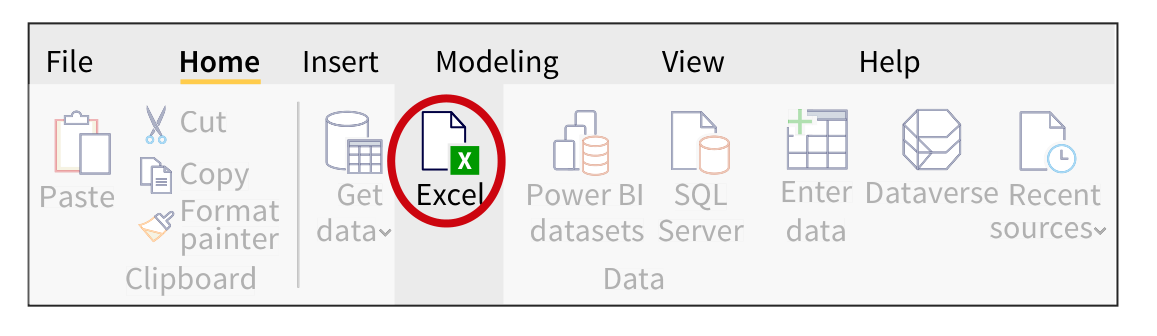
\includegraphics[width=0.95\textwidth,height=0.75\textheight,keepaspectratio]{../textbookForPractice/Figures/Ch_05/ILLUSTRATION 5.49.png}
    \end{figure}
\end{frame}

\begin{frame}{ILLUSTRATION 5.50}

    \begin{figure}[h]
        \centering
        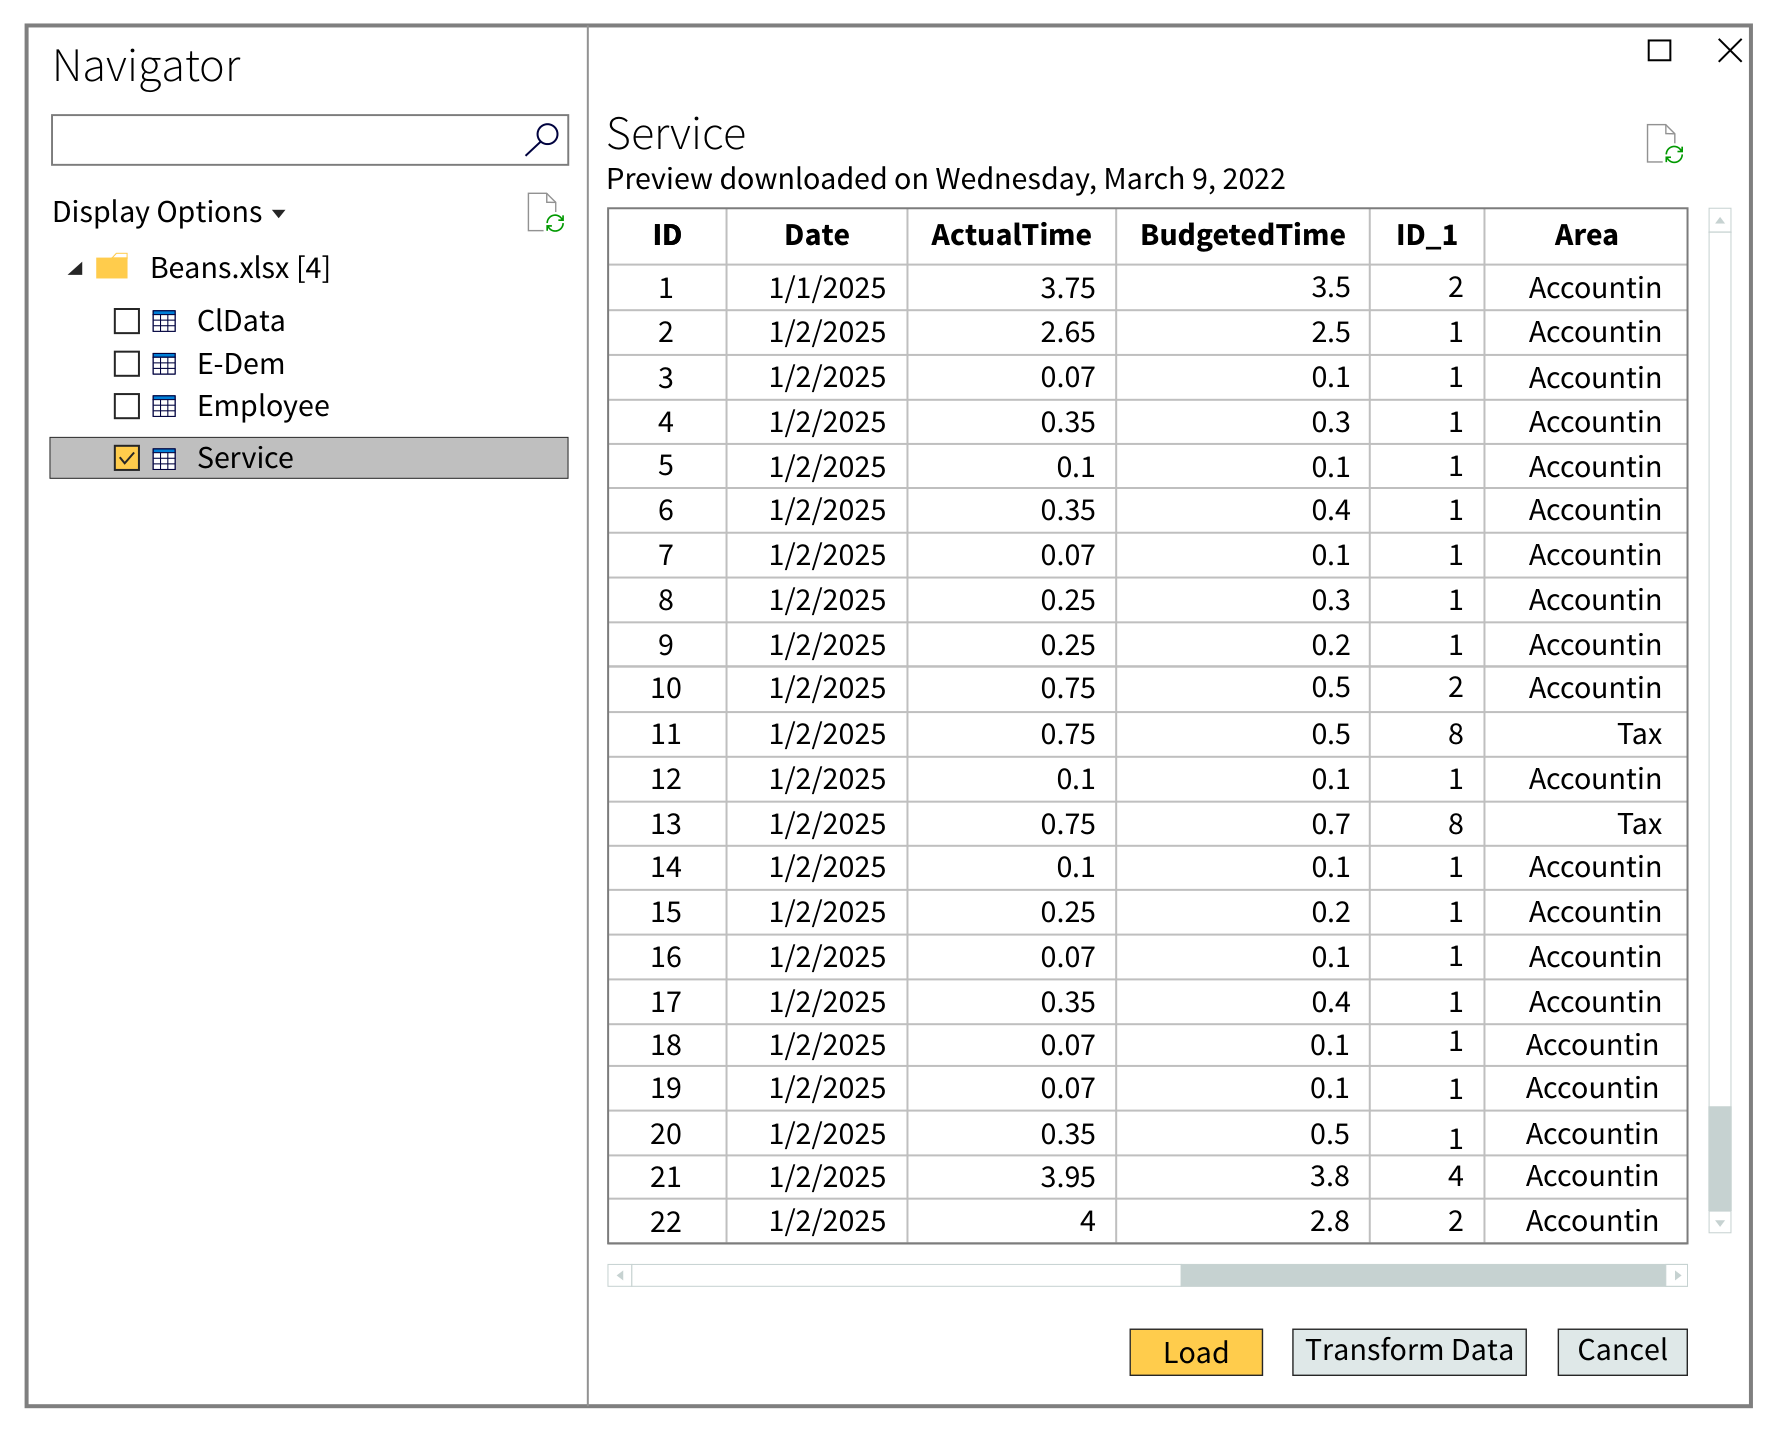
\includegraphics[width=0.95\textwidth,height=0.75\textheight,keepaspectratio]{../textbookForPractice/Figures/Ch_05/ILLUSTRATION 5.50.png}
    \end{figure}
\end{frame}

\begin{frame}{ILLUSTRATION 5.51}

    \begin{figure}[h]
        \centering
        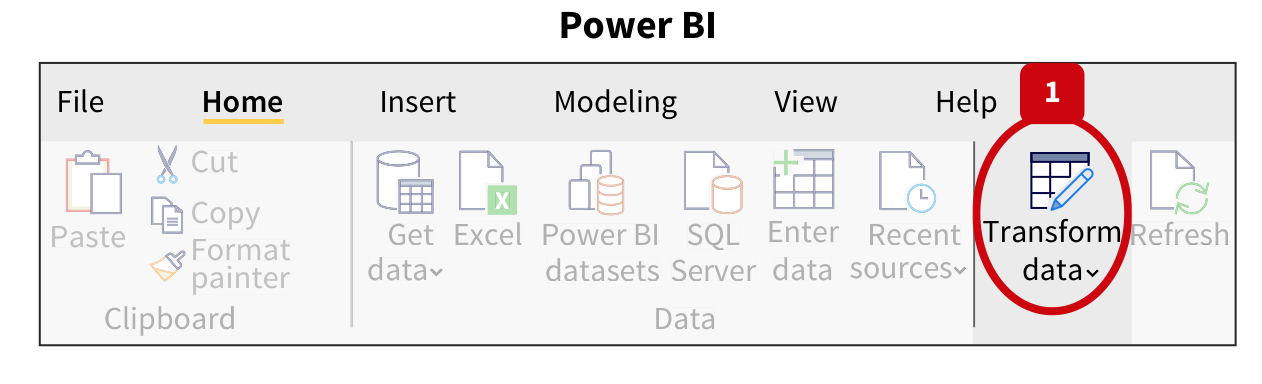
\includegraphics[width=0.95\textwidth,height=0.75\textheight,keepaspectratio]{../textbookForPractice/Figures/Ch_05/ILLUSTRATION 5.51.png}
    \end{figure}
\end{frame}

\begin{frame}{5.7 Áp dụng mẫu cho vấn đề Tải Dữ liệu (Data Loading)}
\begin{itemize}
    \item \textbf{Tải ban đầu (Initial Load):} Nạp toàn bộ dữ liệu lịch sử vào một Data Warehouse mới tinh. Thường tốn nhiều thời gian.
    \item \textbf{Tải tăng dần (Incremental Load):} Chỉ nạp những giao dịch mới phát sinh, chạy định kỳ hàng ngày/hàng giờ.
    \item \textbf{Tải làm mới (Full Refresh):} Xóa toàn bộ dữ liệu cũ và nạp lại toàn bộ dữ liệu mới. Chỉ dùng cho các bảng nhỏ và ít thay đổi.
    \item \textbf{Kiểm tra tính toàn vẹn (Integrity Checks):} Phải đảm bảo số dòng của bảng Nguồn (Source) khớp với bảng Đích (Destination) sau khi tải.
\end{itemize}
\end{frame}

\begin{frame}{ILLUSTRATION 5.52}

    \begin{figure}[h]
        \centering
        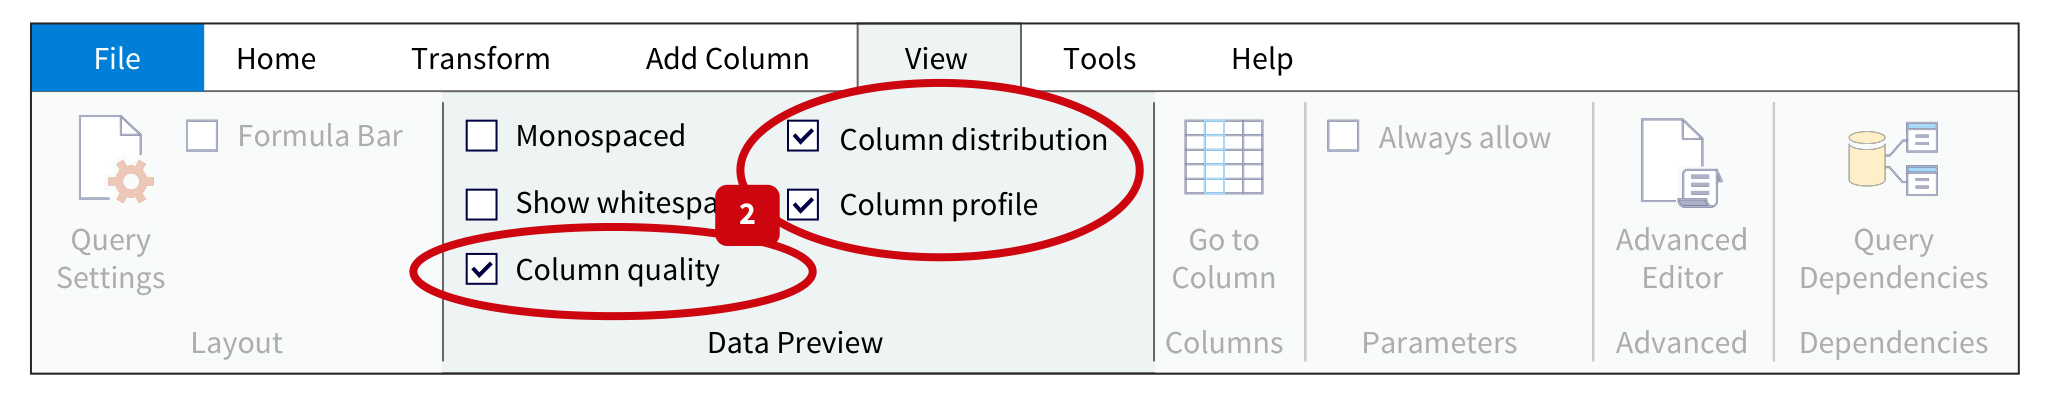
\includegraphics[width=0.95\textwidth,height=0.75\textheight,keepaspectratio]{../textbookForPractice/Figures/Ch_05/ILLUSTRATION 5.52.png}
    \end{figure}
\end{frame}

\begin{frame}{ILLUSTRATION 5.53}

    \begin{figure}[h]
        \centering
        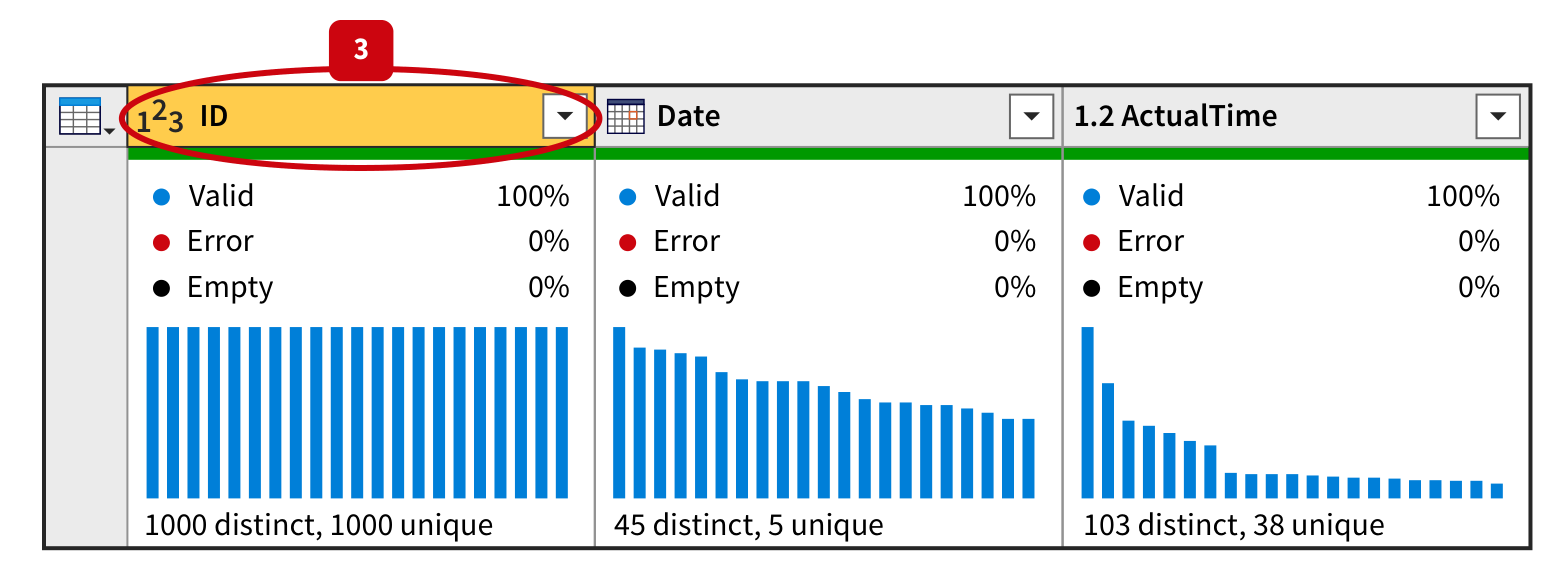
\includegraphics[width=0.95\textwidth,height=0.75\textheight,keepaspectratio]{../textbookForPractice/Figures/Ch_05/ILLUSTRATION 5.53.png}
    \end{figure}
\end{frame}

\begin{frame}{ILLUSTRATION 5.54}

    \begin{figure}[h]
        \centering
        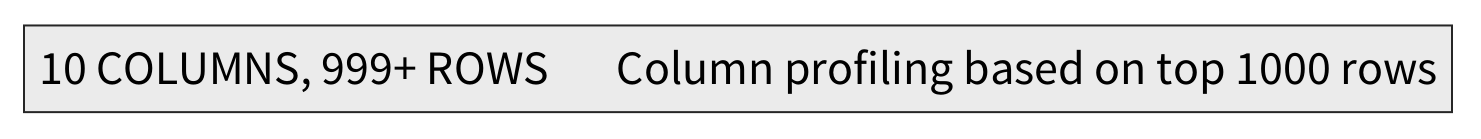
\includegraphics[width=0.95\textwidth,height=0.75\textheight,keepaspectratio]{../textbookForPractice/Figures/Ch_05/ILLUSTRATION 5.54.png}
    \end{figure}
\end{frame}

\begin{frame}{ILLUSTRATION 5.55}

    \begin{figure}[h]
        \centering
        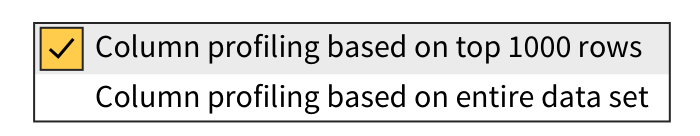
\includegraphics[width=0.95\textwidth,height=0.75\textheight,keepaspectratio]{../textbookForPractice/Figures/Ch_05/ILLUSTRATION 5.55.png}
    \end{figure}
\end{frame}

\begin{frame}{ILLUSTRATION 5.56}

    \begin{figure}[h]
        \centering
        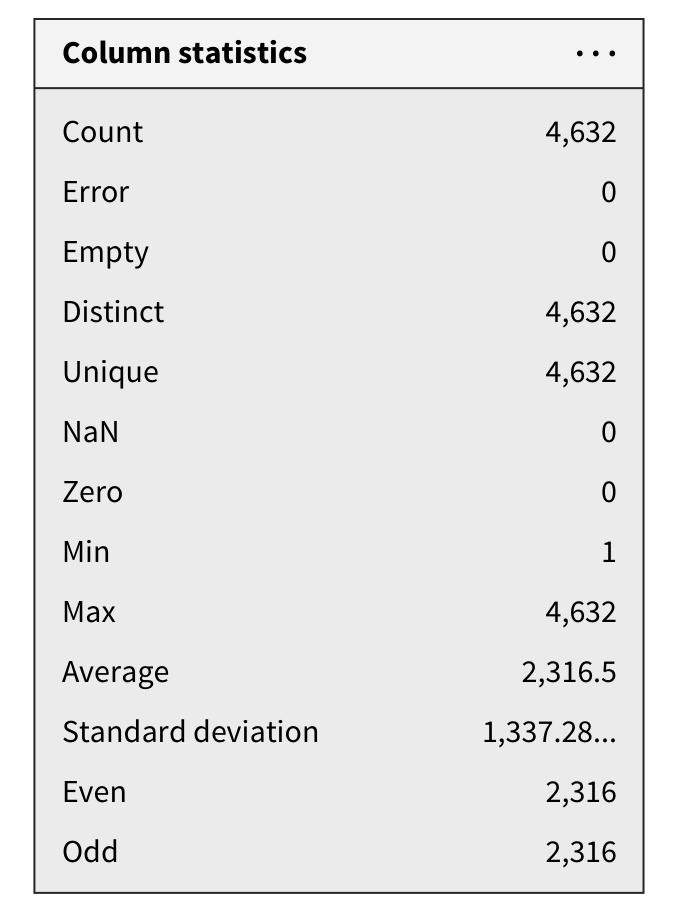
\includegraphics[width=0.95\textwidth,height=0.75\textheight,keepaspectratio]{../textbookForPractice/Figures/Ch_05/ILLUSTRATION 5.56.png}
    \end{figure}
\end{frame}

\begin{frame}{ILLUSTRATION 5.57}

    \begin{figure}[h]
        \centering
        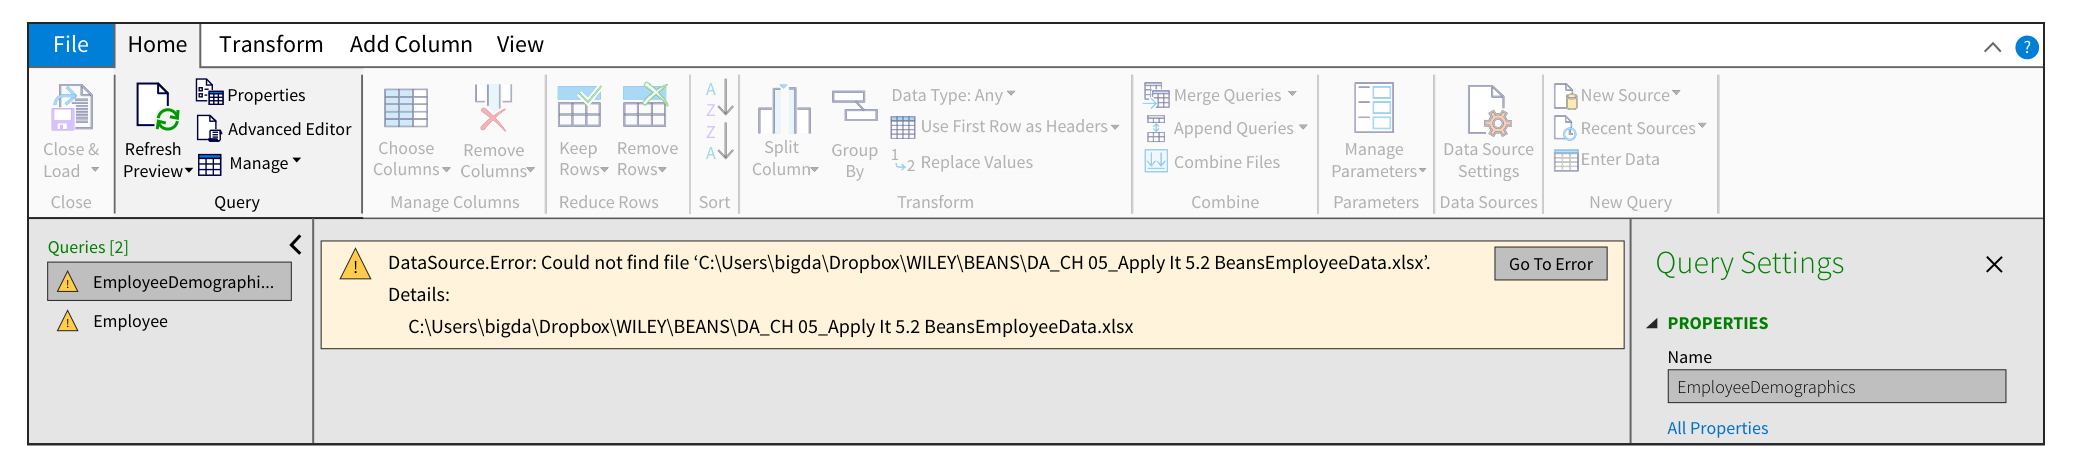
\includegraphics[width=0.95\textwidth,height=0.75\textheight,keepaspectratio]{../textbookForPractice/Figures/Ch_05/ILLUSTRATION 5.57.png}
    \end{figure}
\end{frame}

\begin{frame}{Các Tình huống Apply It}
\begin{center}
    \Huge \textbf{Apply It}
\end{center}
\end{frame}

\begin{frame}{ILLUSTRATION 5.58}

    \begin{figure}[h]
        \centering
        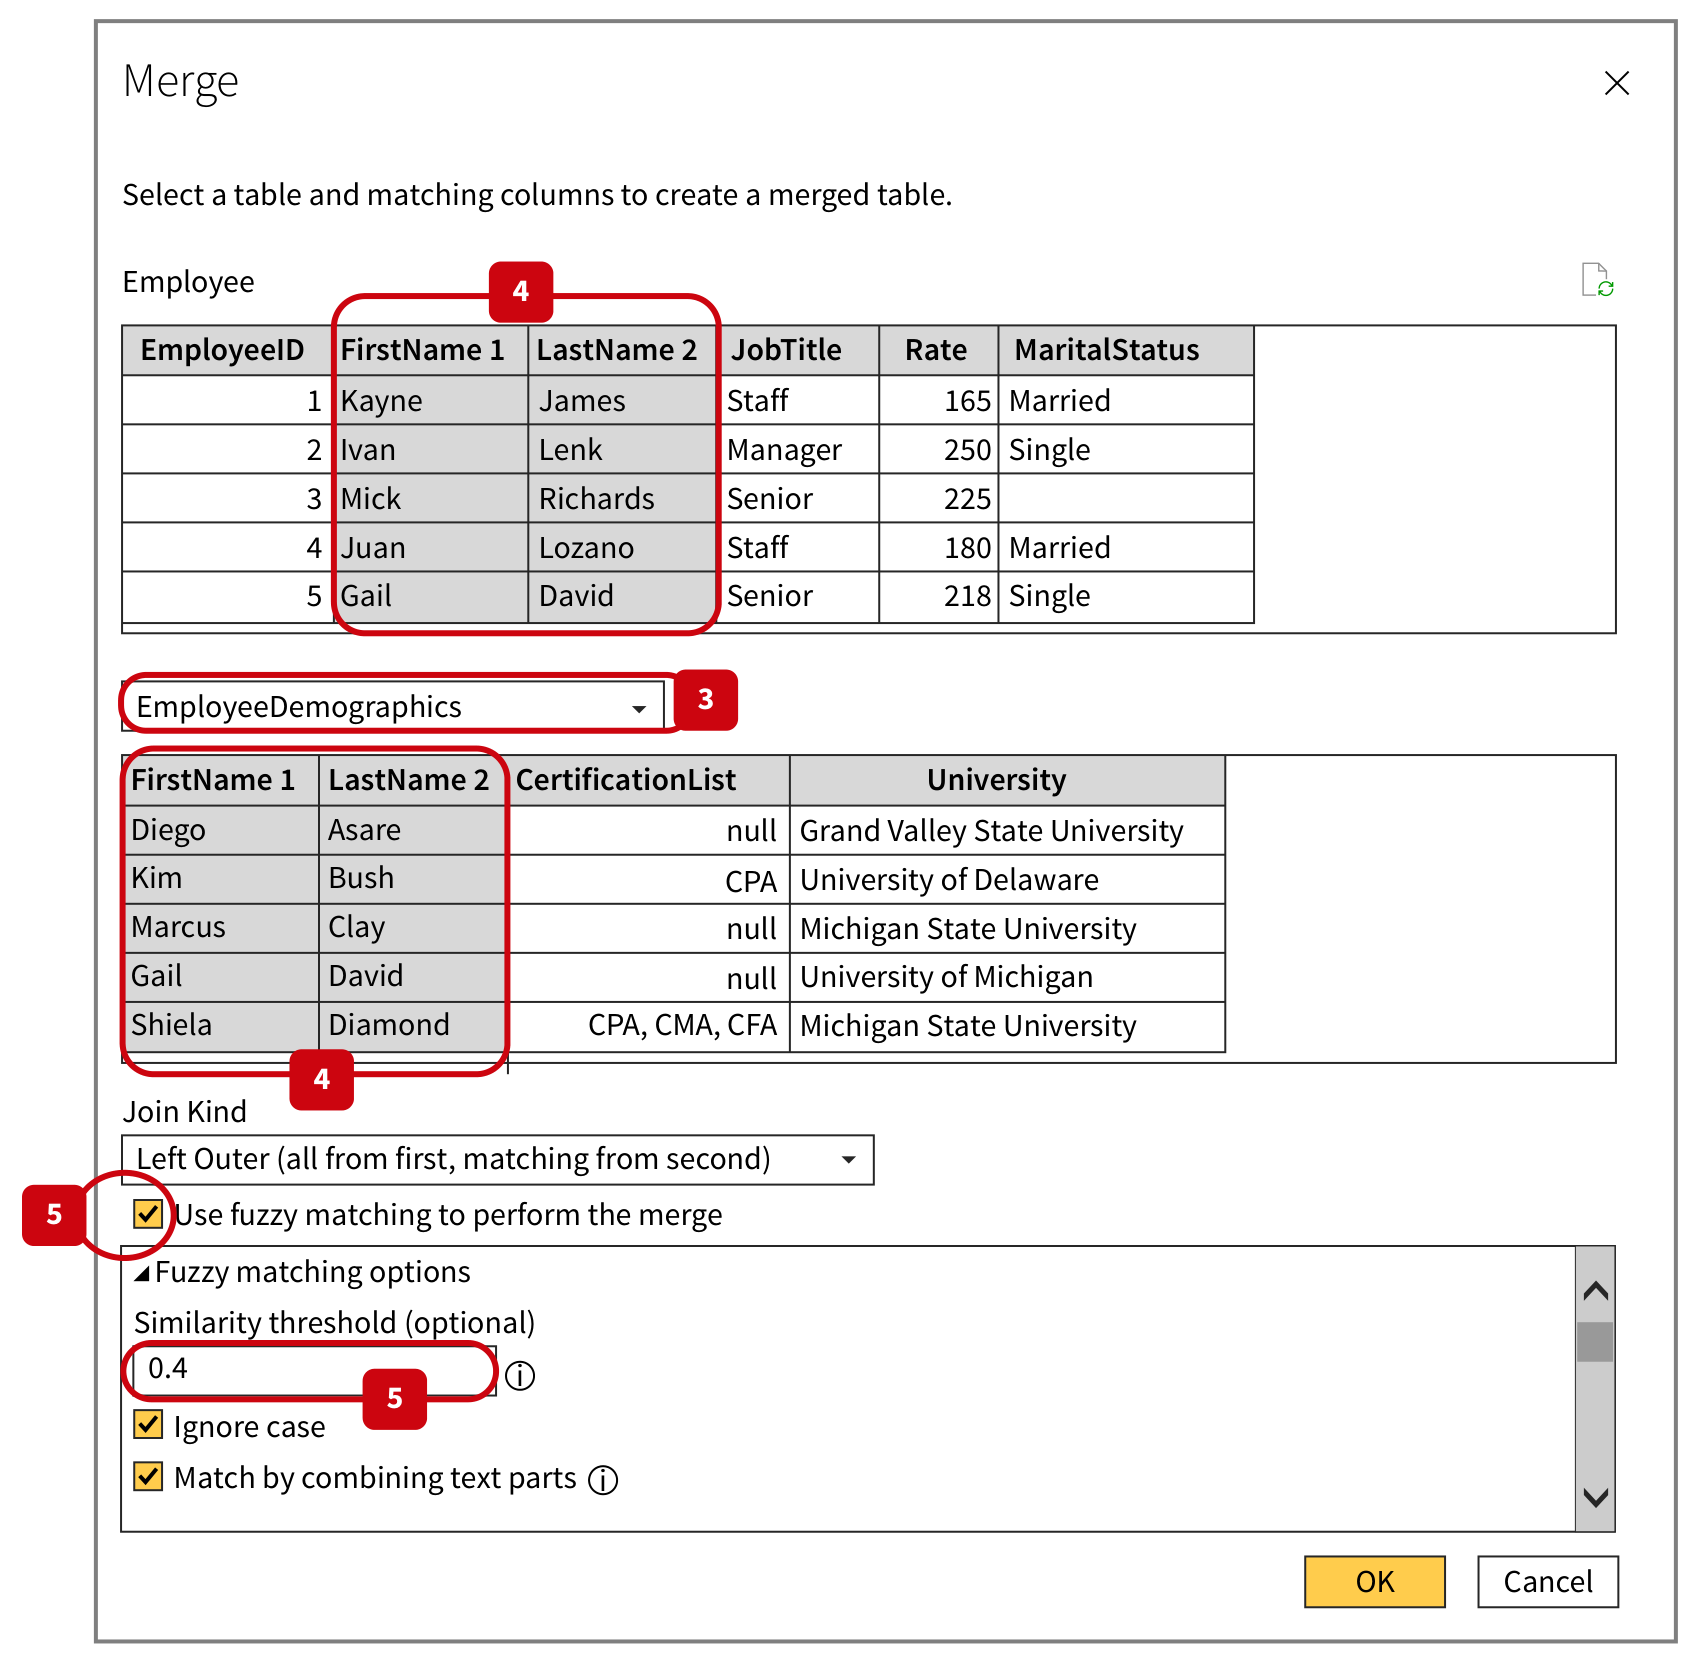
\includegraphics[width=0.95\textwidth,height=0.75\textheight,keepaspectratio]{../textbookForPractice/Figures/Ch_05/ILLUSTRATION 5.58.png}
    \end{figure}
\end{frame}

\begin{frame}{ILLUSTRATION 5.59}

    \begin{figure}[h]
        \centering
        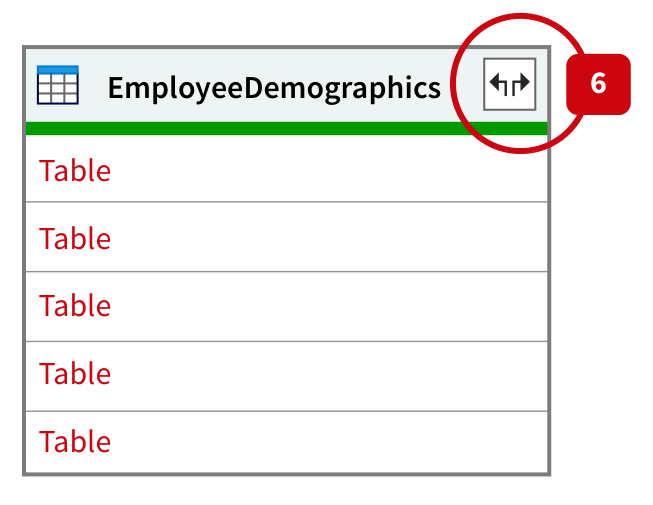
\includegraphics[width=0.95\textwidth,height=0.75\textheight,keepaspectratio]{../textbookForPractice/Figures/Ch_05/ILLUSTRATION 5.59.png}
    \end{figure}
\end{frame}

\begin{frame}{ILLUSTRATION 5.60}

    \begin{figure}[h]
        \centering
        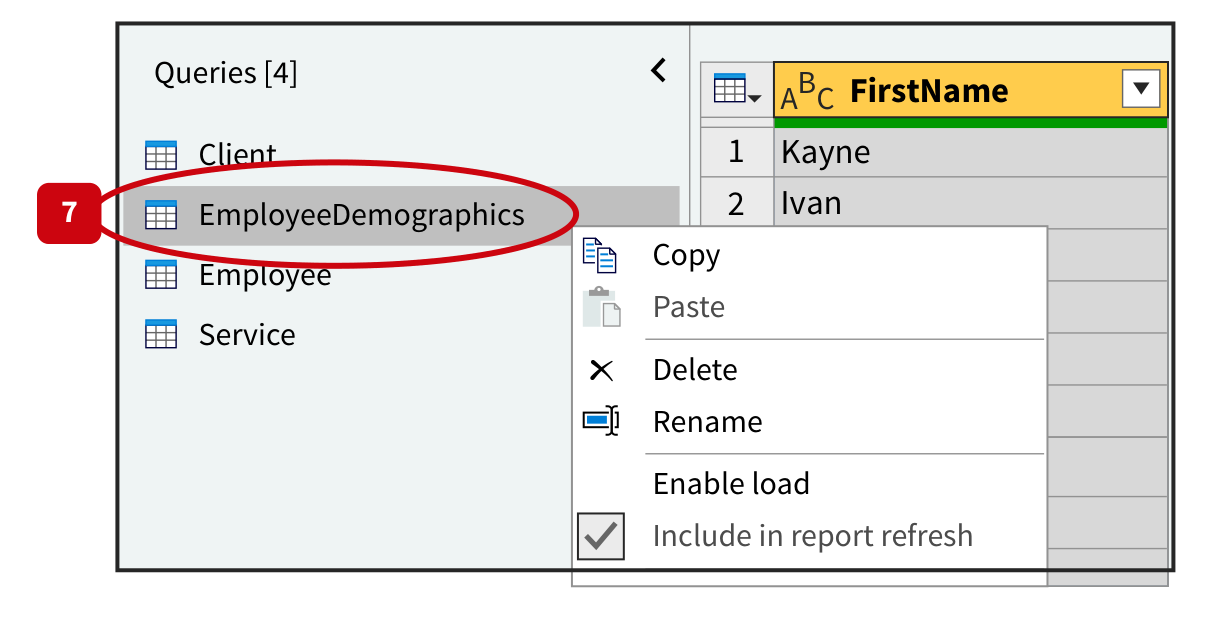
\includegraphics[width=0.95\textwidth,height=0.75\textheight,keepaspectratio]{../textbookForPractice/Figures/Ch_05/ILLUSTRATION 5.60.png}
    \end{figure}
\end{frame}

\begin{frame}{ILLUSTRATION 5.61}

    \begin{figure}[h]
        \centering
        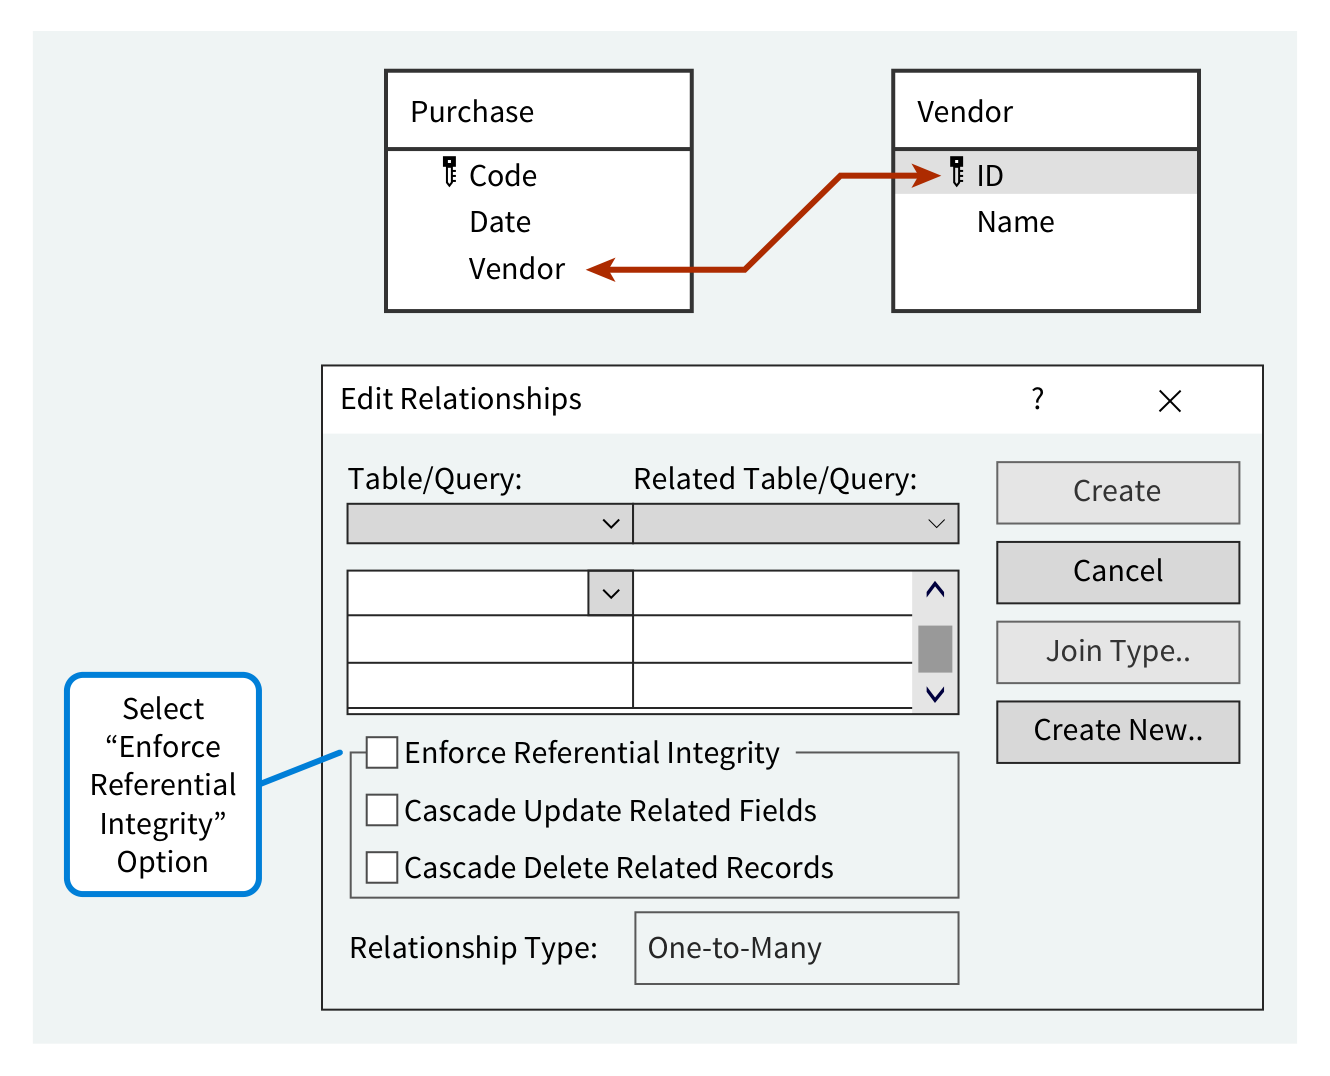
\includegraphics[width=0.95\textwidth,height=0.75\textheight,keepaspectratio]{../textbookForPractice/Figures/Ch_05/ILLUSTRATION 5.61.png}
    \end{figure}
\end{frame}

\begin{frame}{ILLUSTRATION 5.62}

    \begin{figure}[h]
        \centering
        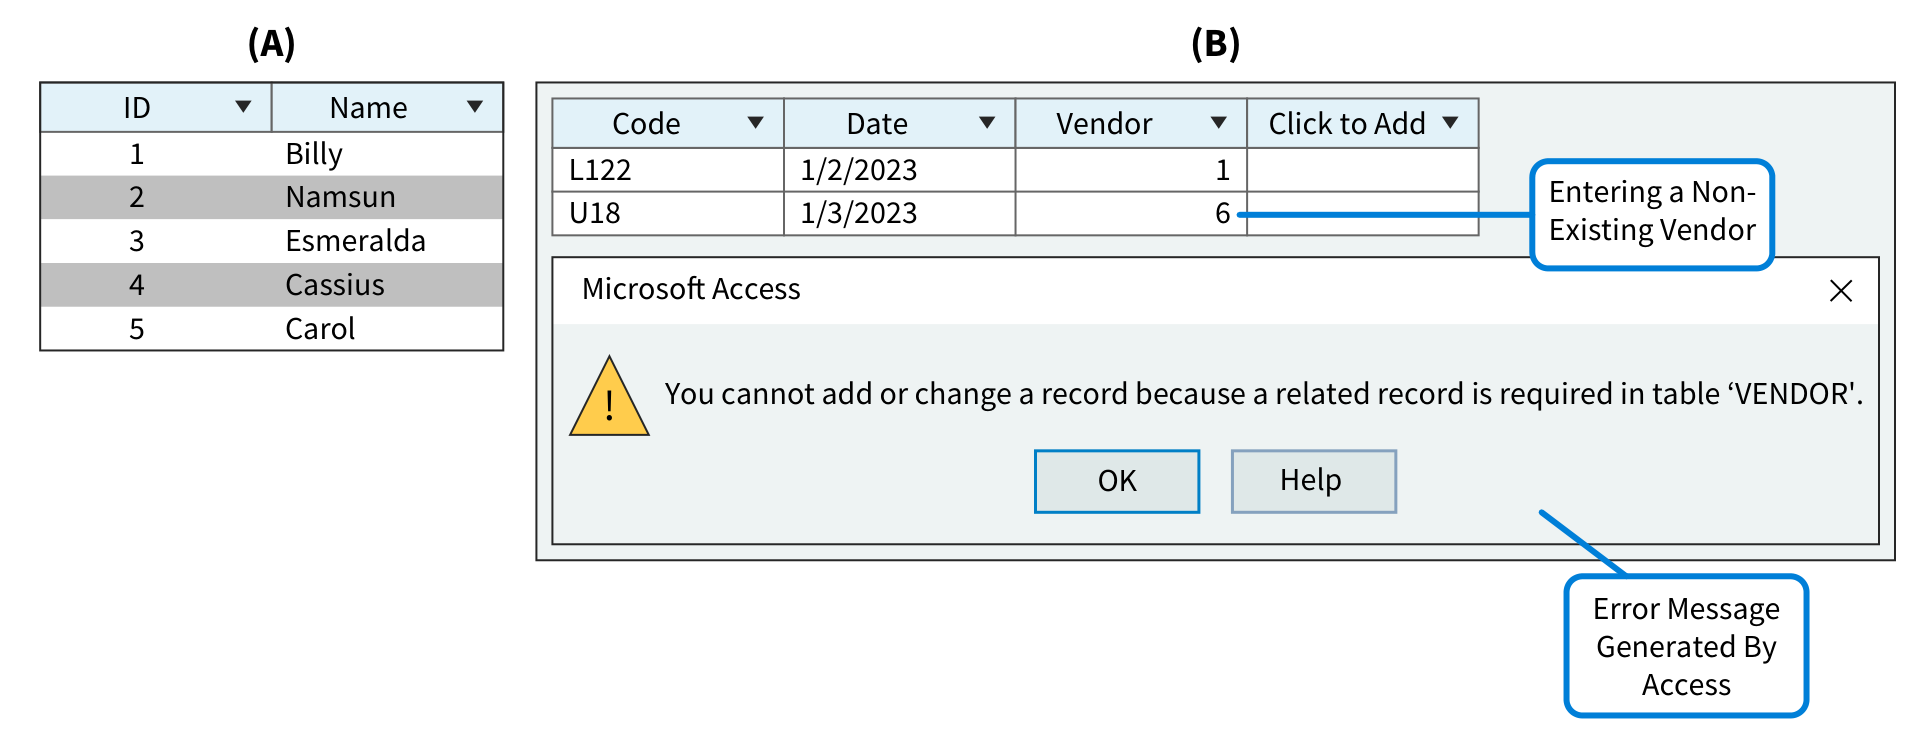
\includegraphics[width=0.95\textwidth,height=0.75\textheight,keepaspectratio]{../textbookForPractice/Figures/Ch_05/ILLUSTRATION 5.62.png}
    \end{figure}
\end{frame}

\begin{frame}{Apply It 5.1}

    \begin{figure}[h]
        \centering
        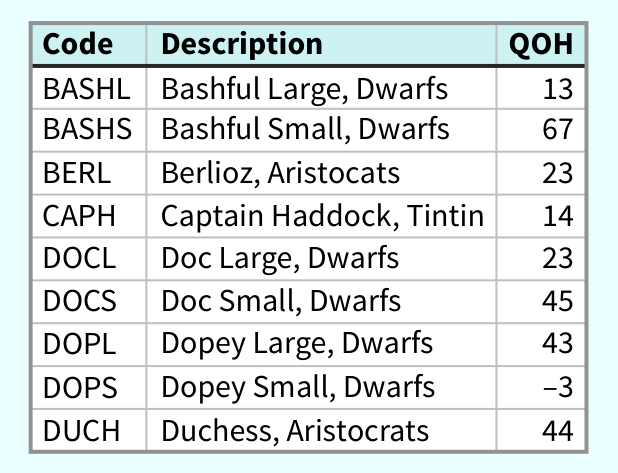
\includegraphics[width=0.95\textwidth,height=0.75\textheight,keepaspectratio]{../textbookForPractice/Figures/Ch_05/Apply It 5.1.png}
    \end{figure}
\end{frame}

\begin{frame}{Apply It 5.2}

    \begin{figure}[h]
        \centering
        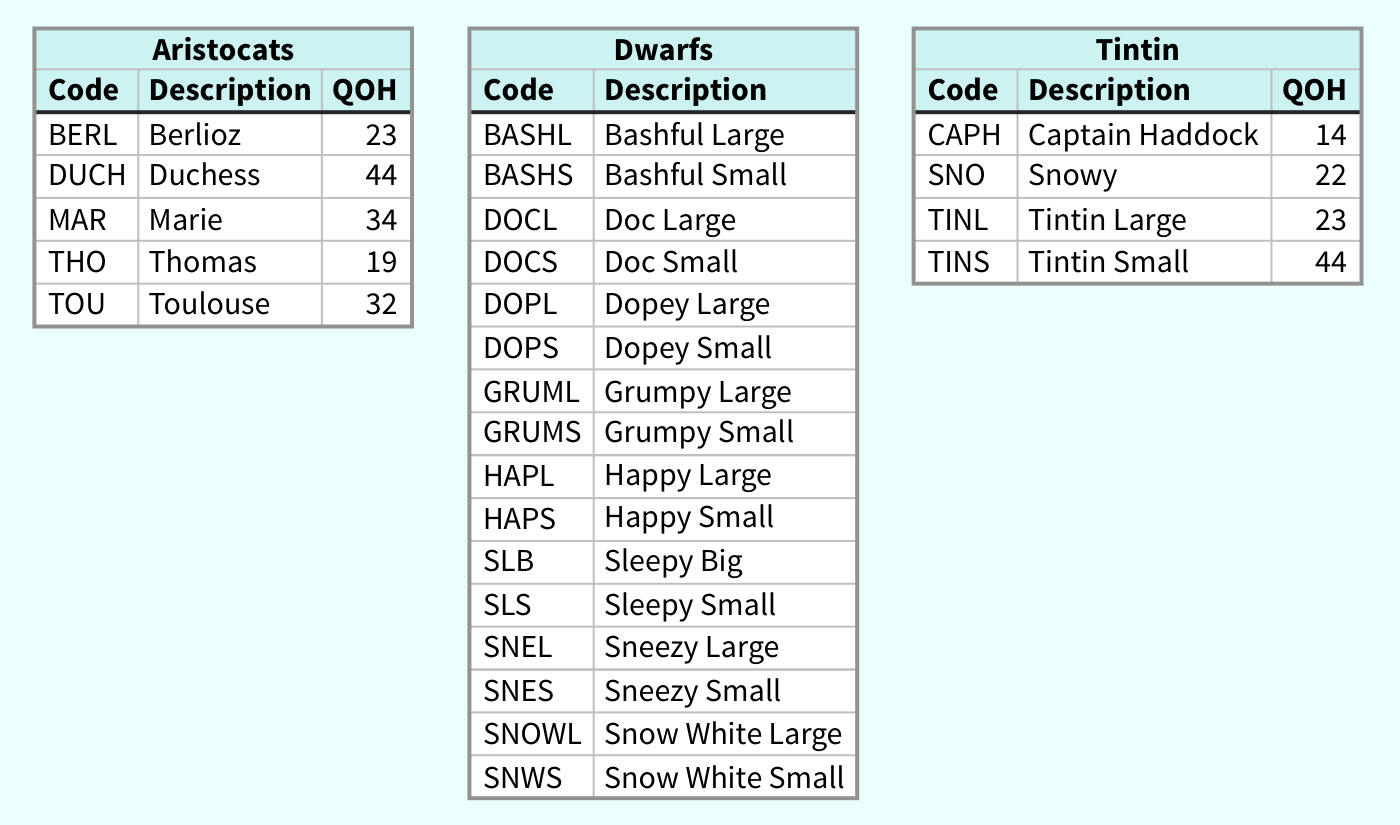
\includegraphics[width=0.95\textwidth,height=0.75\textheight,keepaspectratio]{../textbookForPractice/Figures/Ch_05/Apply It 5.2.png}
    \end{figure}
\end{frame}

\begin{frame}{Apply It 5.3}

    \begin{figure}[h]
        \centering
        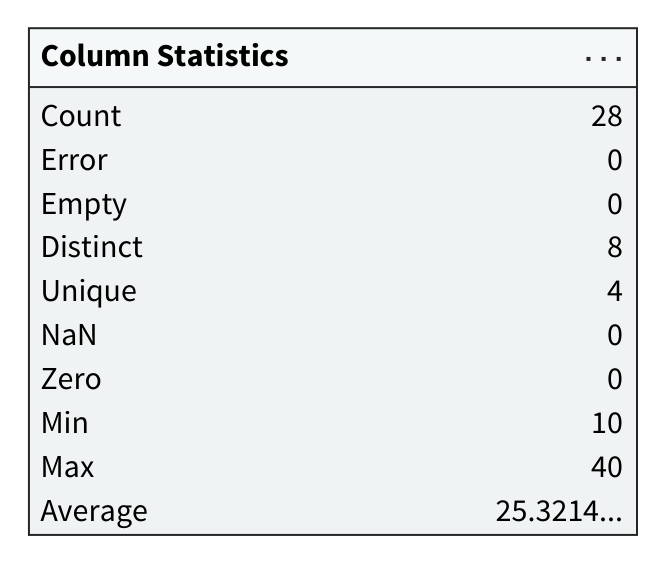
\includegraphics[width=0.95\textwidth,height=0.75\textheight,keepaspectratio]{../textbookForPractice/Figures/Ch_05/Apply It 5.3.png}
    \end{figure}
\end{frame}

\begin{frame}{Apply It 5.5}

    \begin{figure}[h]
        \centering
        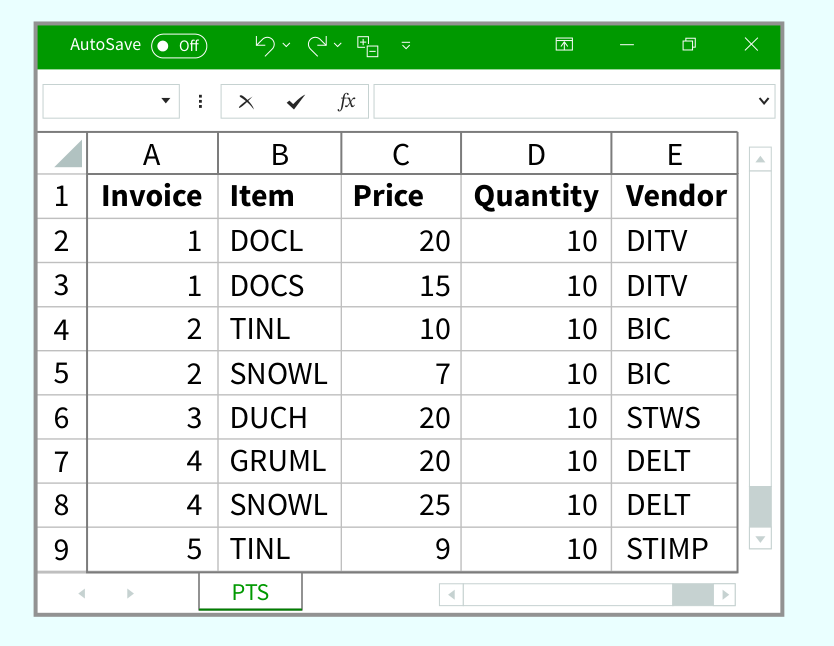
\includegraphics[width=0.95\textwidth,height=0.75\textheight,keepaspectratio]{../textbookForPractice/Figures/Ch_05/Apply It 5.5.png}
    \end{figure}
\end{frame}

\begin{frame}{Apply It 5.6}

    \begin{figure}[h]
        \centering
        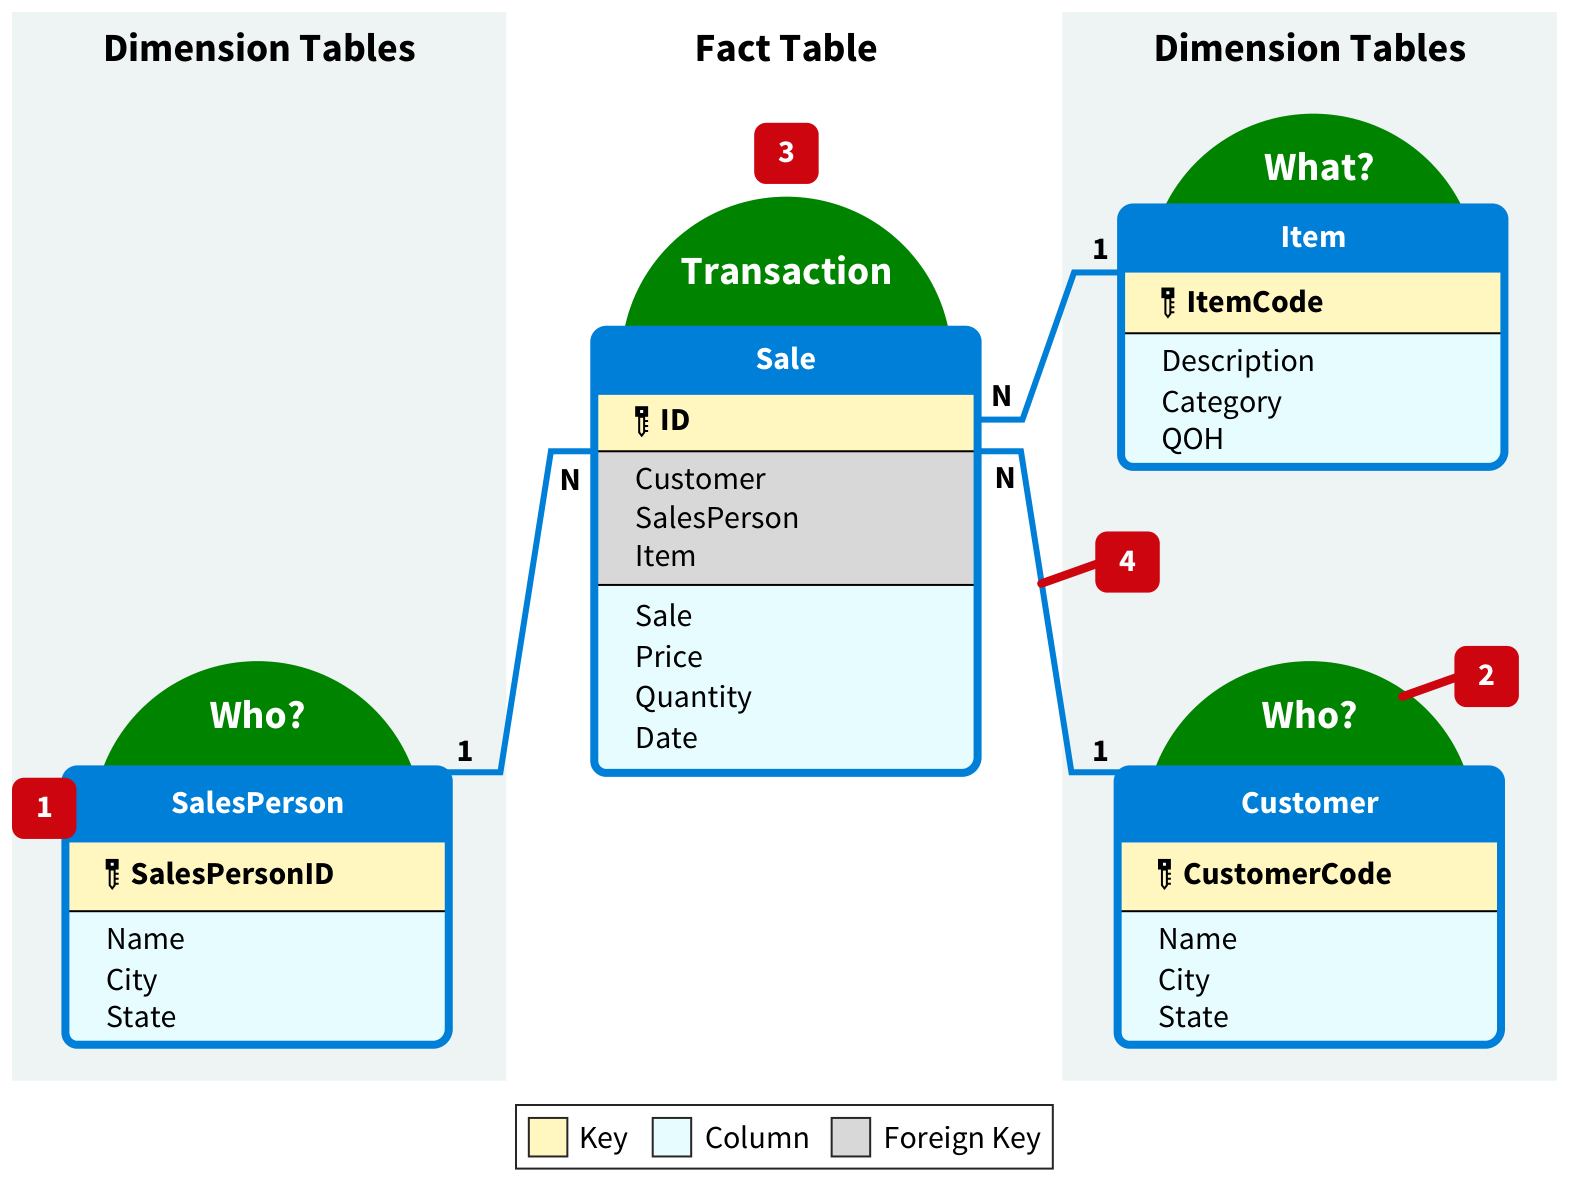
\includegraphics[width=0.95\textwidth,height=0.75\textheight,keepaspectratio]{../textbookForPractice/Figures/Ch_05/Apply It 5.6.png}
    \end{figure}
\end{frame}

\begin{frame}{Apply It 5.7}

    \begin{figure}[h]
        \centering
        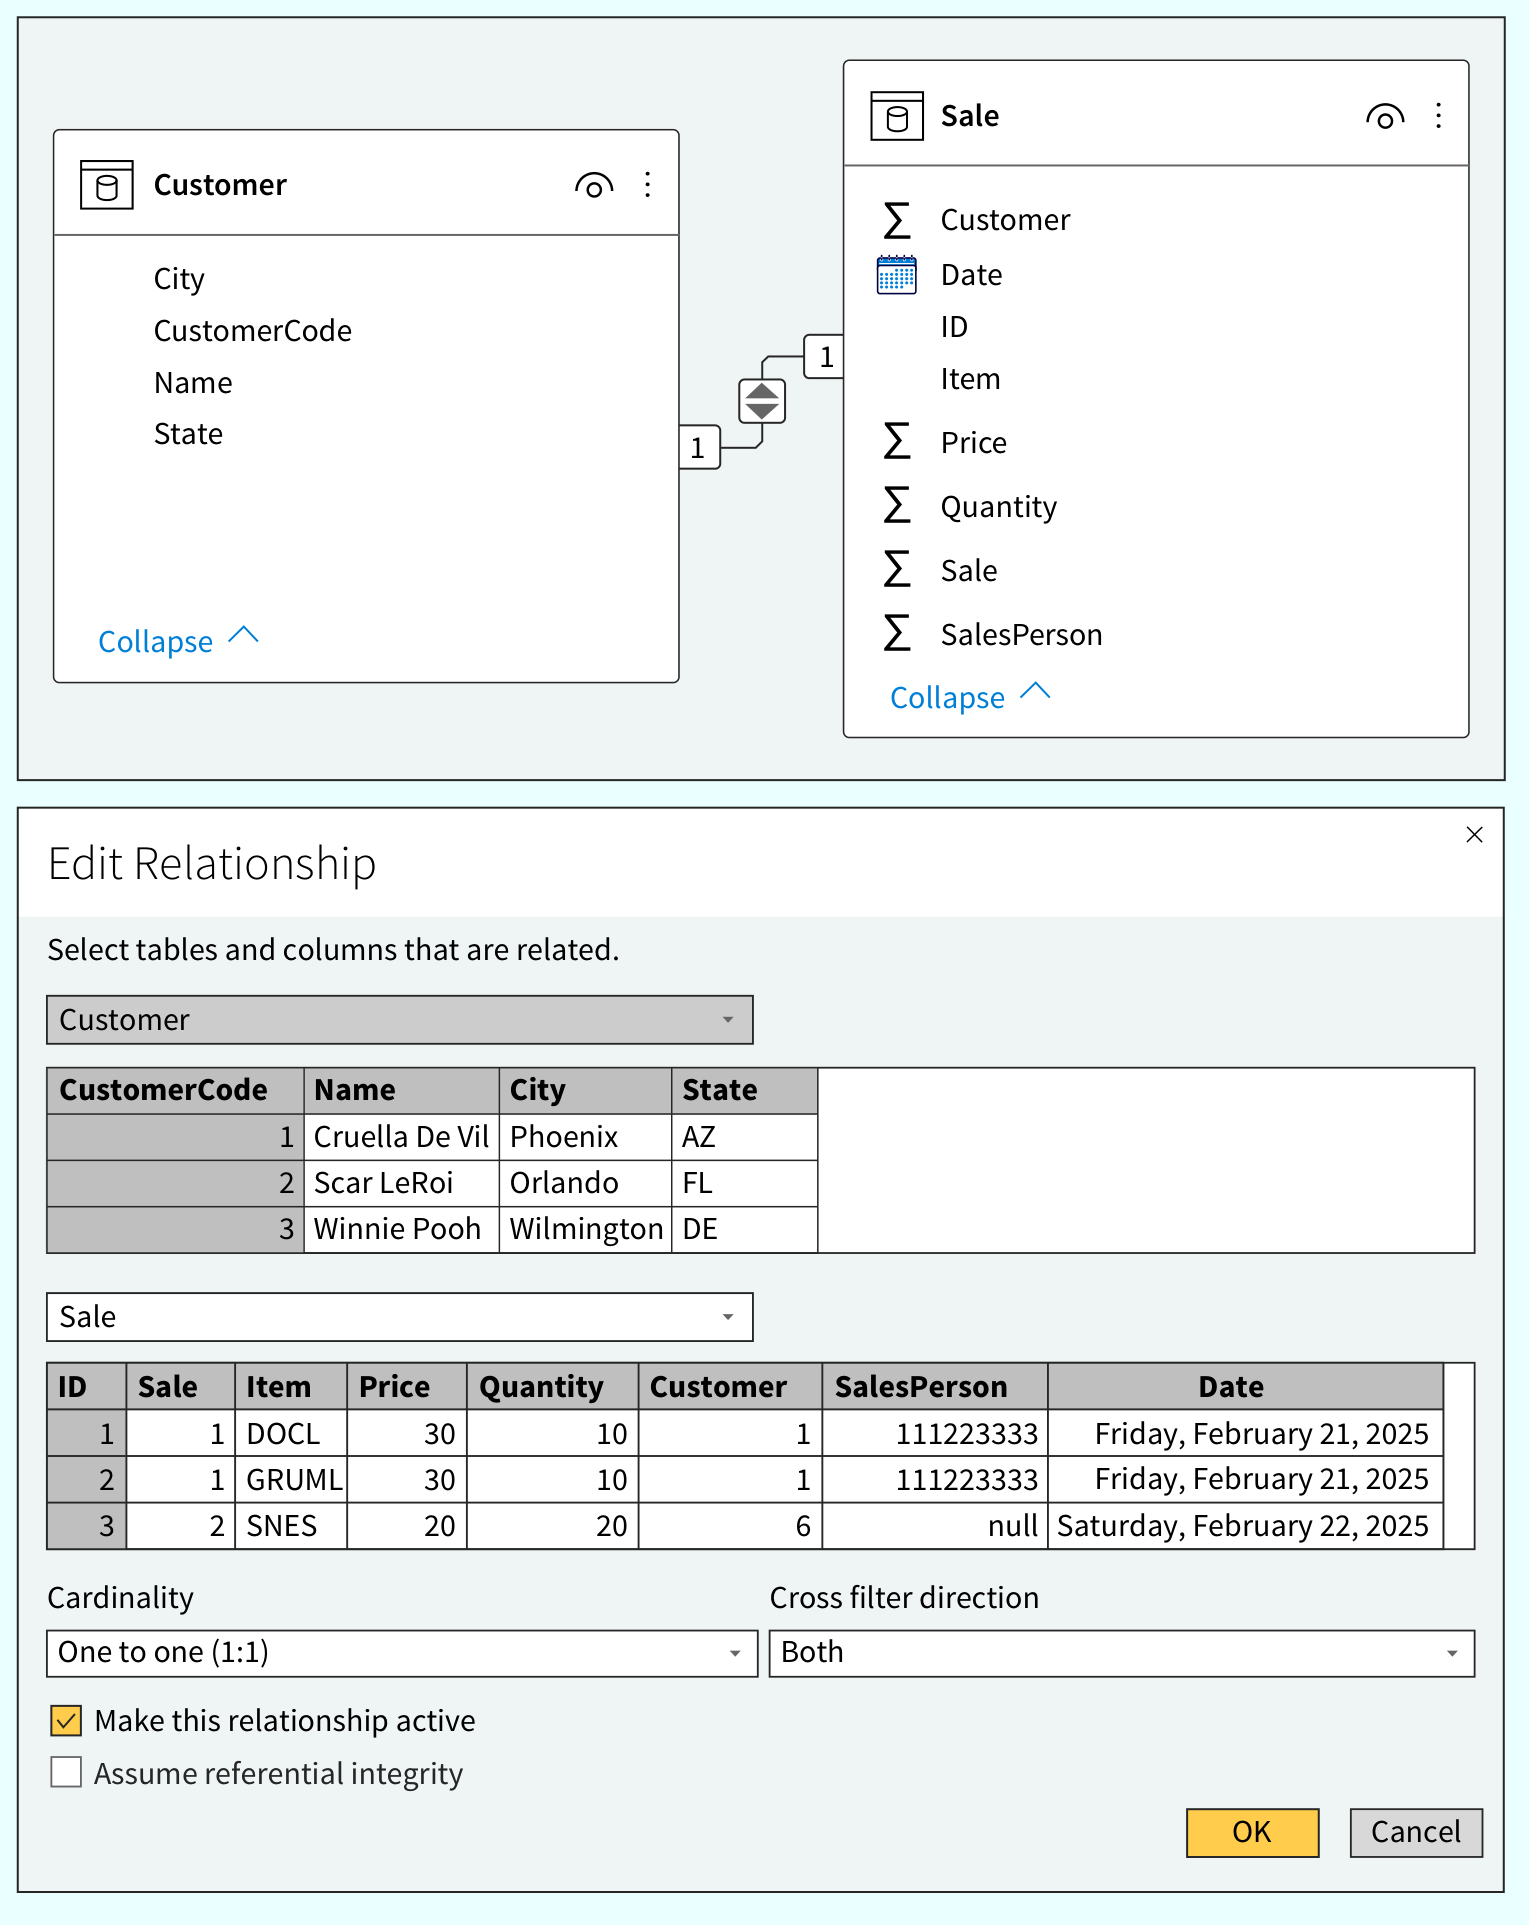
\includegraphics[width=0.95\textwidth,height=0.75\textheight,keepaspectratio]{../textbookForPractice/Figures/Ch_05/Apply It 5.7.png}
    \end{figure}
\end{frame}

\begin{frame}{Phần Bài tập Ngắn (Brief Exercises)}
\begin{center}
    \Huge \textbf{Brief Exercises}
\end{center}
\end{frame}

\begin{frame}{BE 5.1 \& BE 5.2}
    \begin{columns}
        \begin{column}{0.5\textwidth}
            \begin{figure}[h]
                \centering
                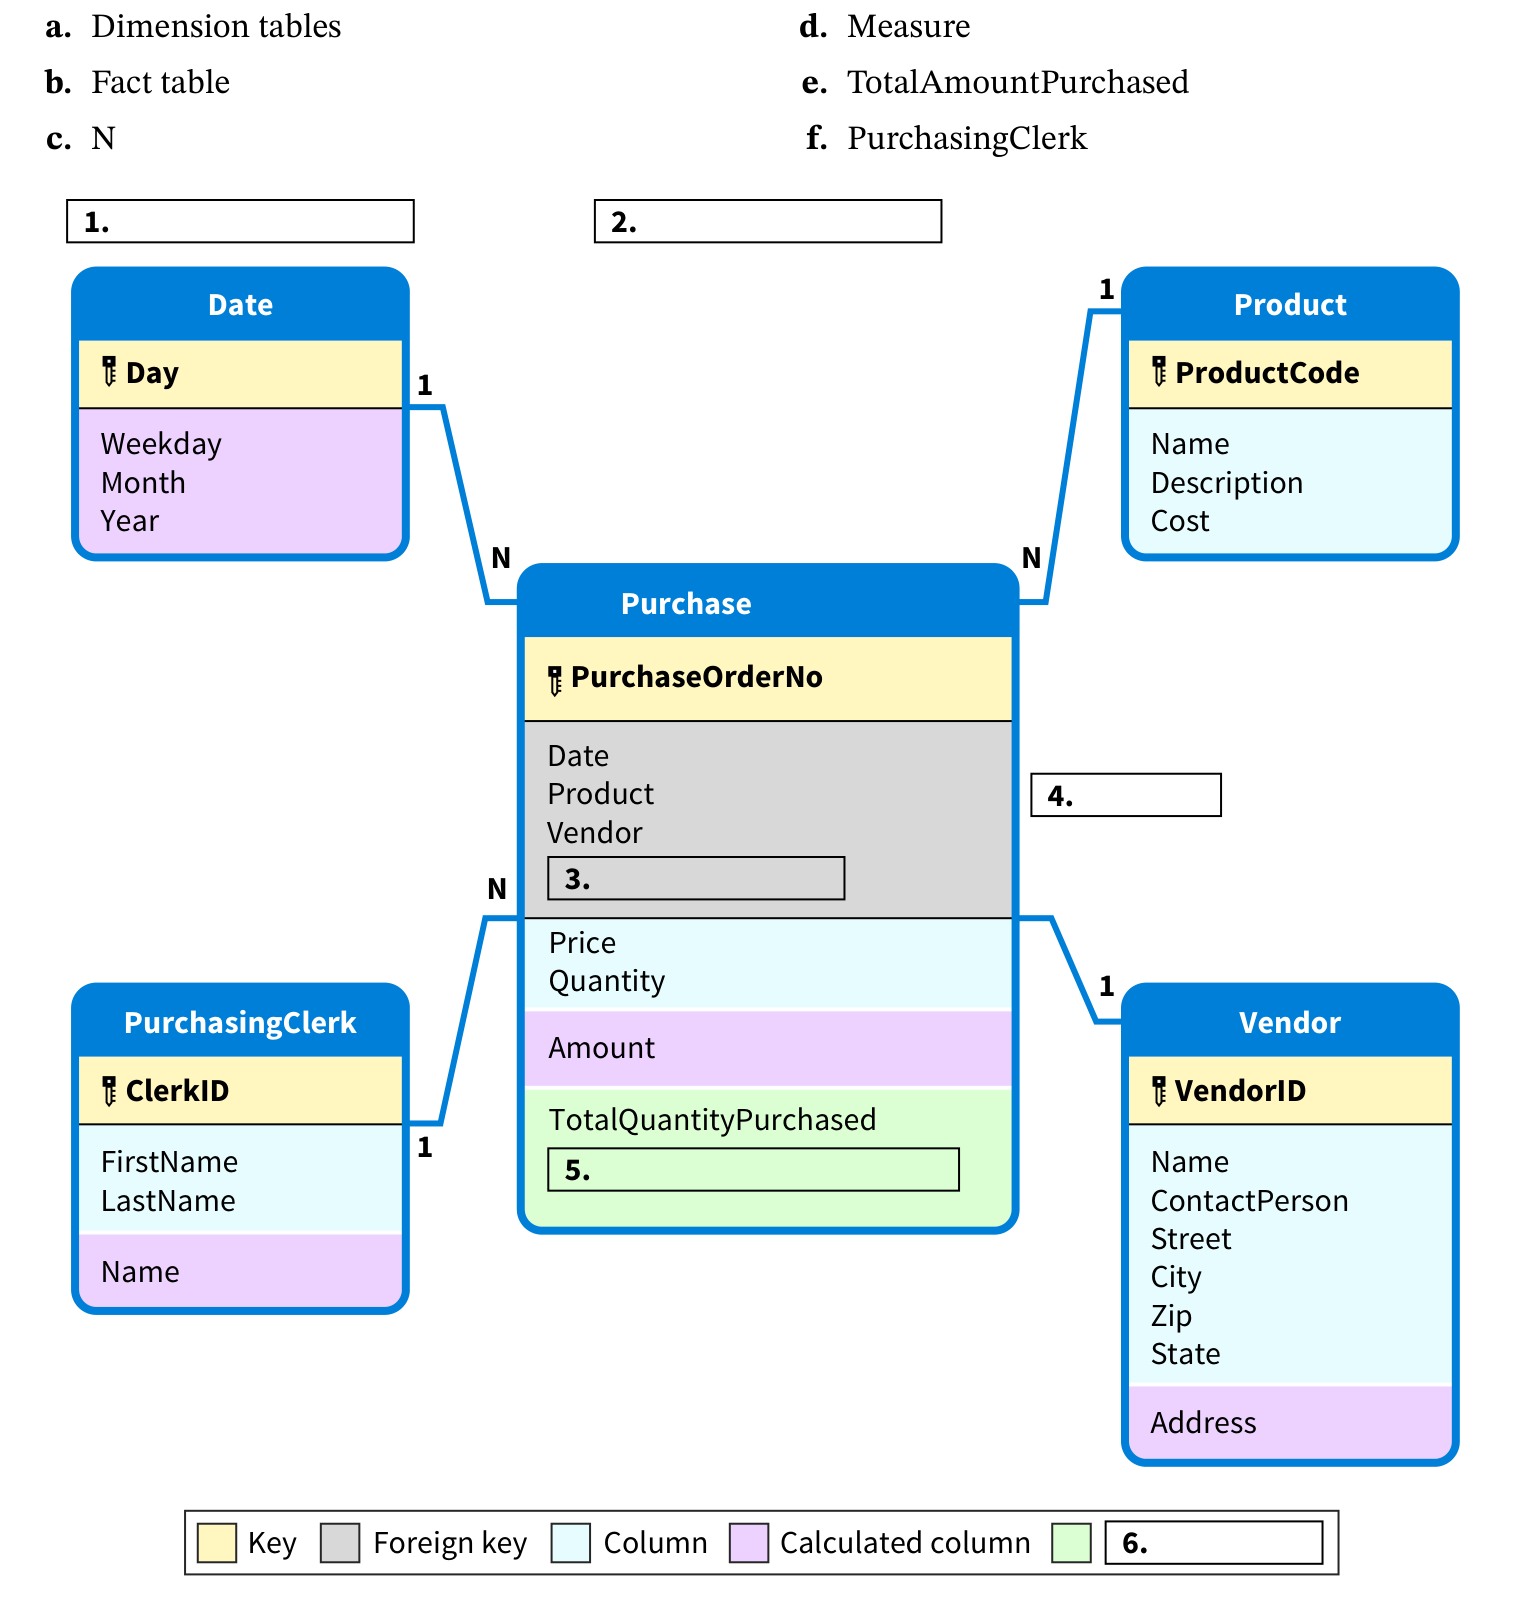
\includegraphics[width=\textwidth,height=0.7\textheight,keepaspectratio]{../textbookForPractice/Figures/Ch_05/BE 5.1.png}
            \end{figure}
        \end{column}
        \begin{column}{0.5\textwidth}
            \begin{figure}[h]
                \centering
                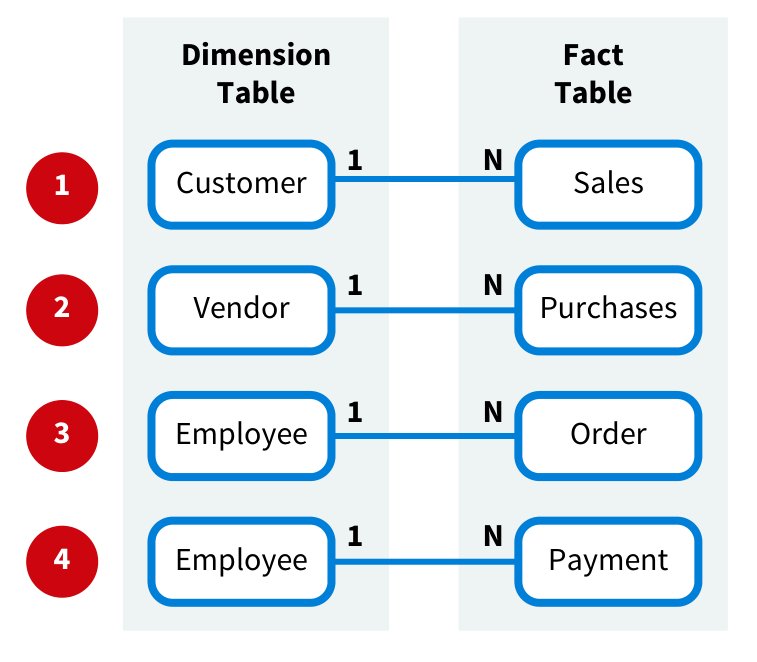
\includegraphics[width=\textwidth,height=0.7\textheight,keepaspectratio]{../textbookForPractice/Figures/Ch_05/BE 5.2.png}
            \end{figure}
        \end{column}
    \end{columns}
\end{frame}

\begin{frame}{BE 5.3 \& BE 5.4}
    \begin{columns}
        \begin{column}{0.5\textwidth}
            \begin{figure}[h]
                \centering
                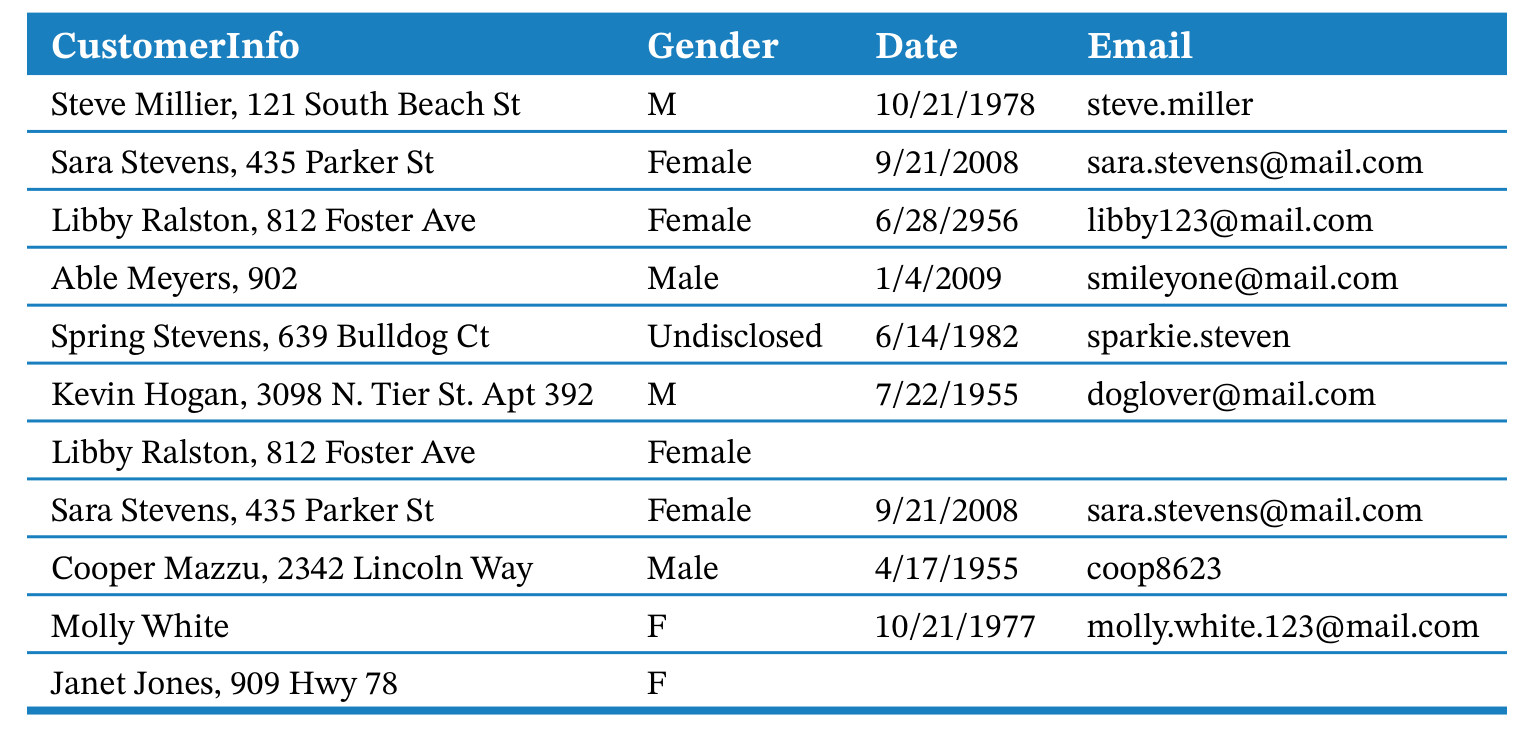
\includegraphics[width=\textwidth,height=0.7\textheight,keepaspectratio]{../textbookForPractice/Figures/Ch_05/BE 5.3.png}
            \end{figure}
        \end{column}
        \begin{column}{0.5\textwidth}
            \begin{figure}[h]
                \centering
                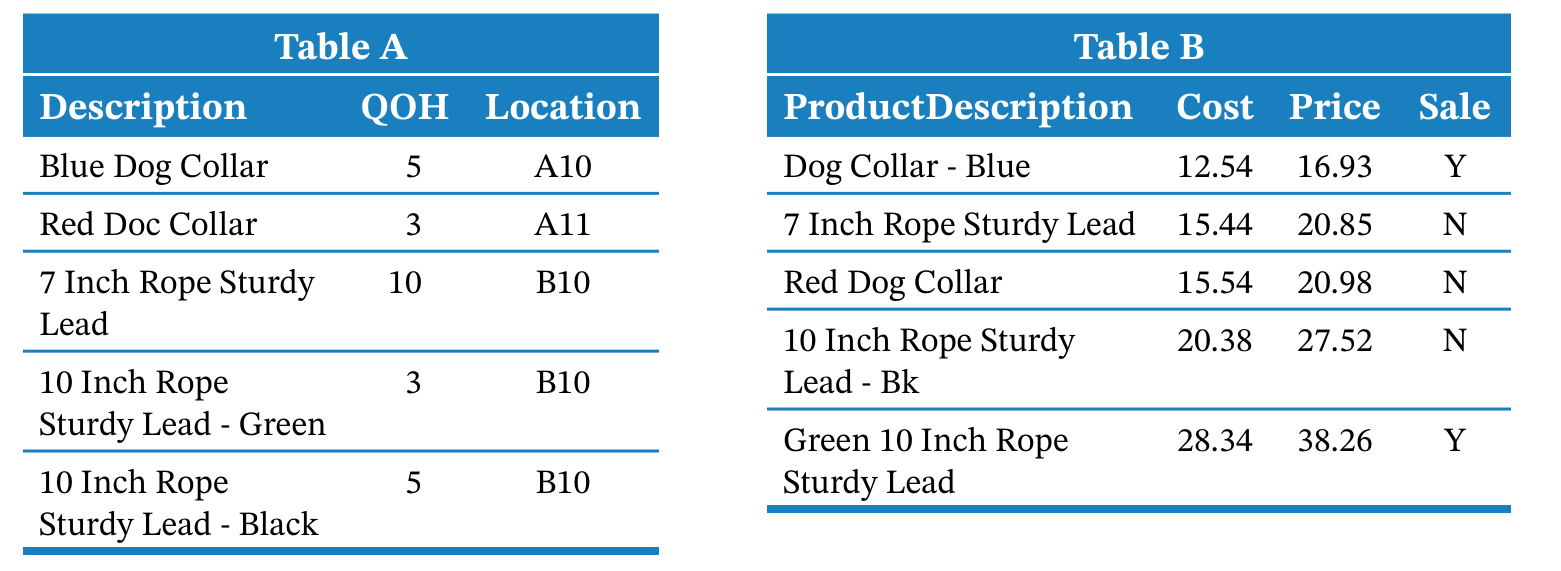
\includegraphics[width=\textwidth,height=0.7\textheight,keepaspectratio]{../textbookForPractice/Figures/Ch_05/BE 5.4.png}
            \end{figure}
        \end{column}
    \end{columns}
\end{frame}

\begin{frame}{BE 5.5 \& BE 5.6}
    \begin{columns}
        \begin{column}{0.5\textwidth}
            \begin{figure}[h]
                \centering
                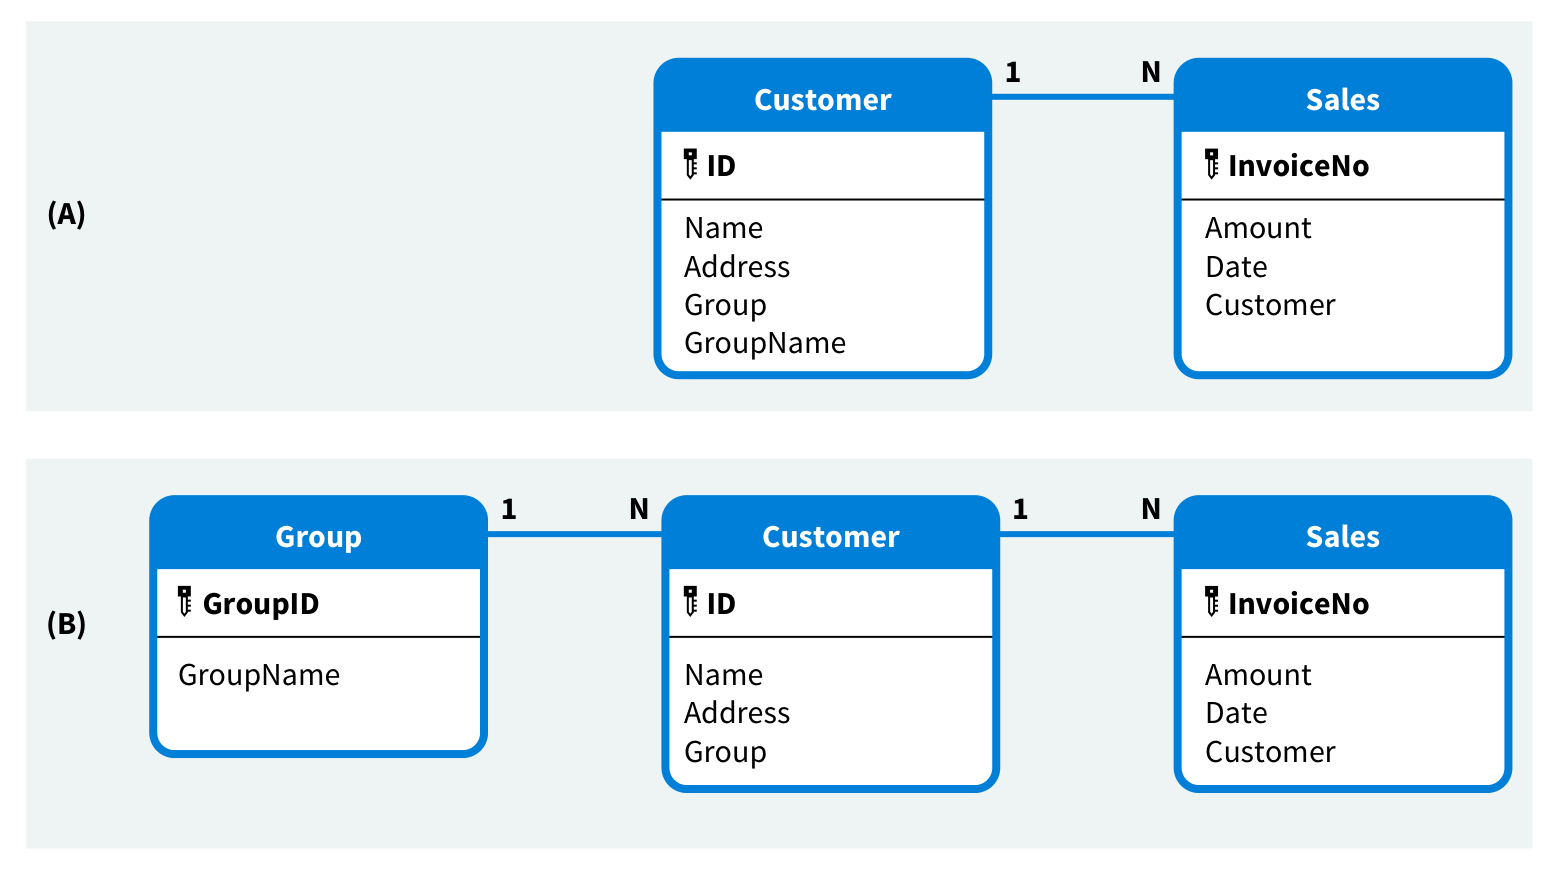
\includegraphics[width=\textwidth,height=0.7\textheight,keepaspectratio]{../textbookForPractice/Figures/Ch_05/BE 5.5.png}
            \end{figure}
        \end{column}
        \begin{column}{0.5\textwidth}
            \begin{figure}[h]
                \centering
                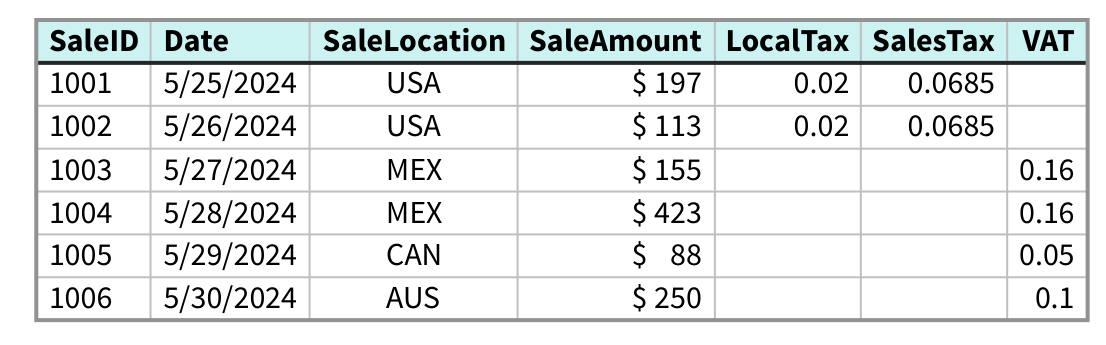
\includegraphics[width=\textwidth,height=0.7\textheight,keepaspectratio]{../textbookForPractice/Figures/Ch_05/BE 5.6.png}
            \end{figure}
        \end{column}
    \end{columns}
\end{frame}

\begin{frame}{BE 5.13 \& BE 5.15}
    \begin{columns}
        \begin{column}{0.5\textwidth}
            \begin{figure}[h]
                \centering
                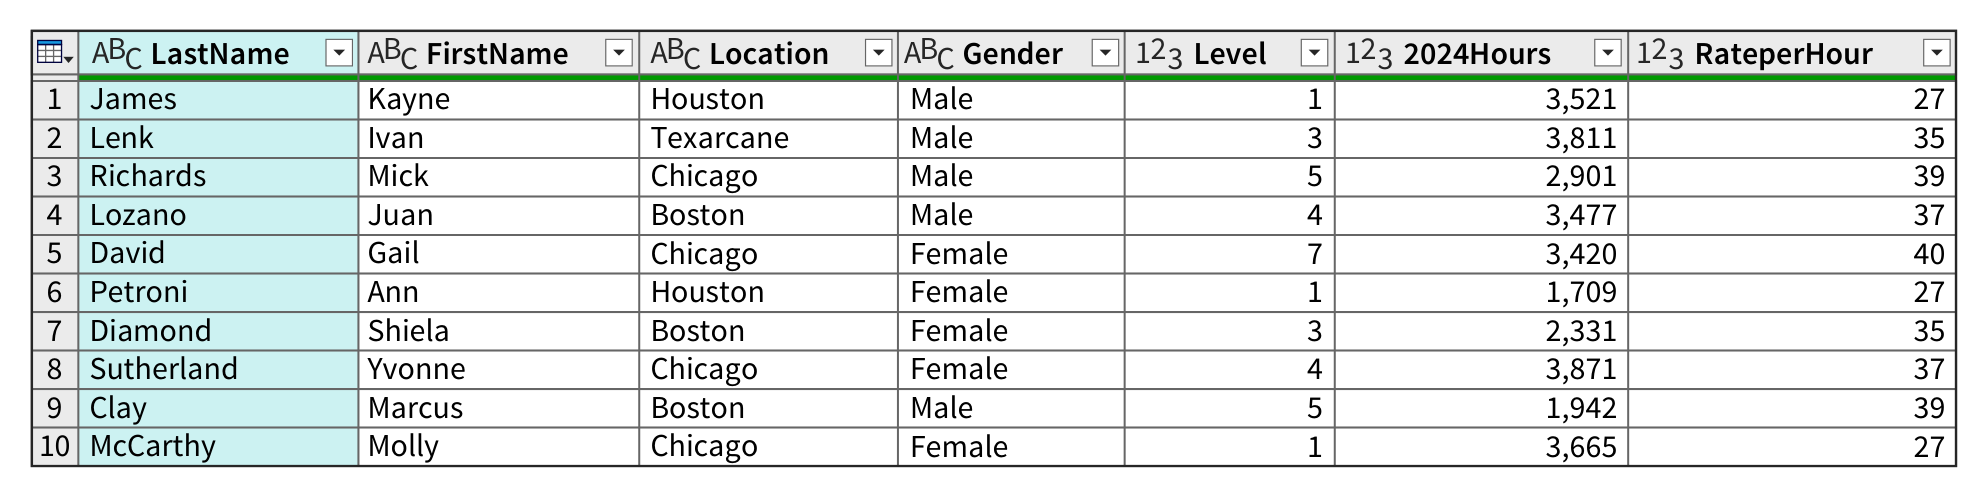
\includegraphics[width=\textwidth,height=0.7\textheight,keepaspectratio]{../textbookForPractice/Figures/Ch_05/BE 5.13.png}
            \end{figure}
        \end{column}
        \begin{column}{0.5\textwidth}
            \begin{figure}[h]
                \centering
                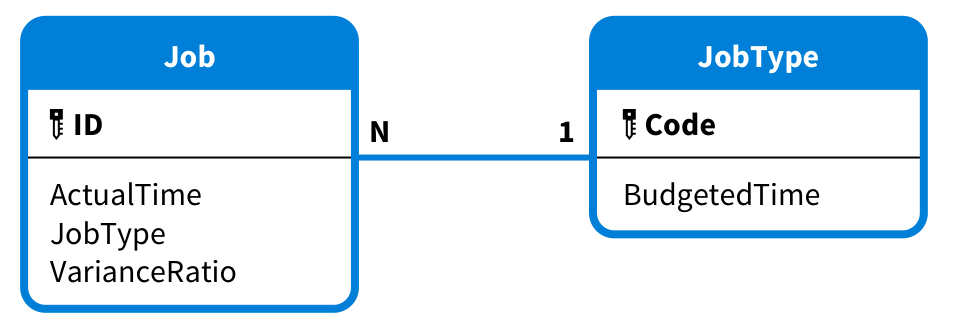
\includegraphics[width=\textwidth,height=0.7\textheight,keepaspectratio]{../textbookForPractice/Figures/Ch_05/BE 5.15.png}
            \end{figure}
        \end{column}
    \end{columns}
\end{frame}

\begin{frame}{BE 5.16}

    \begin{figure}[h]
        \centering
        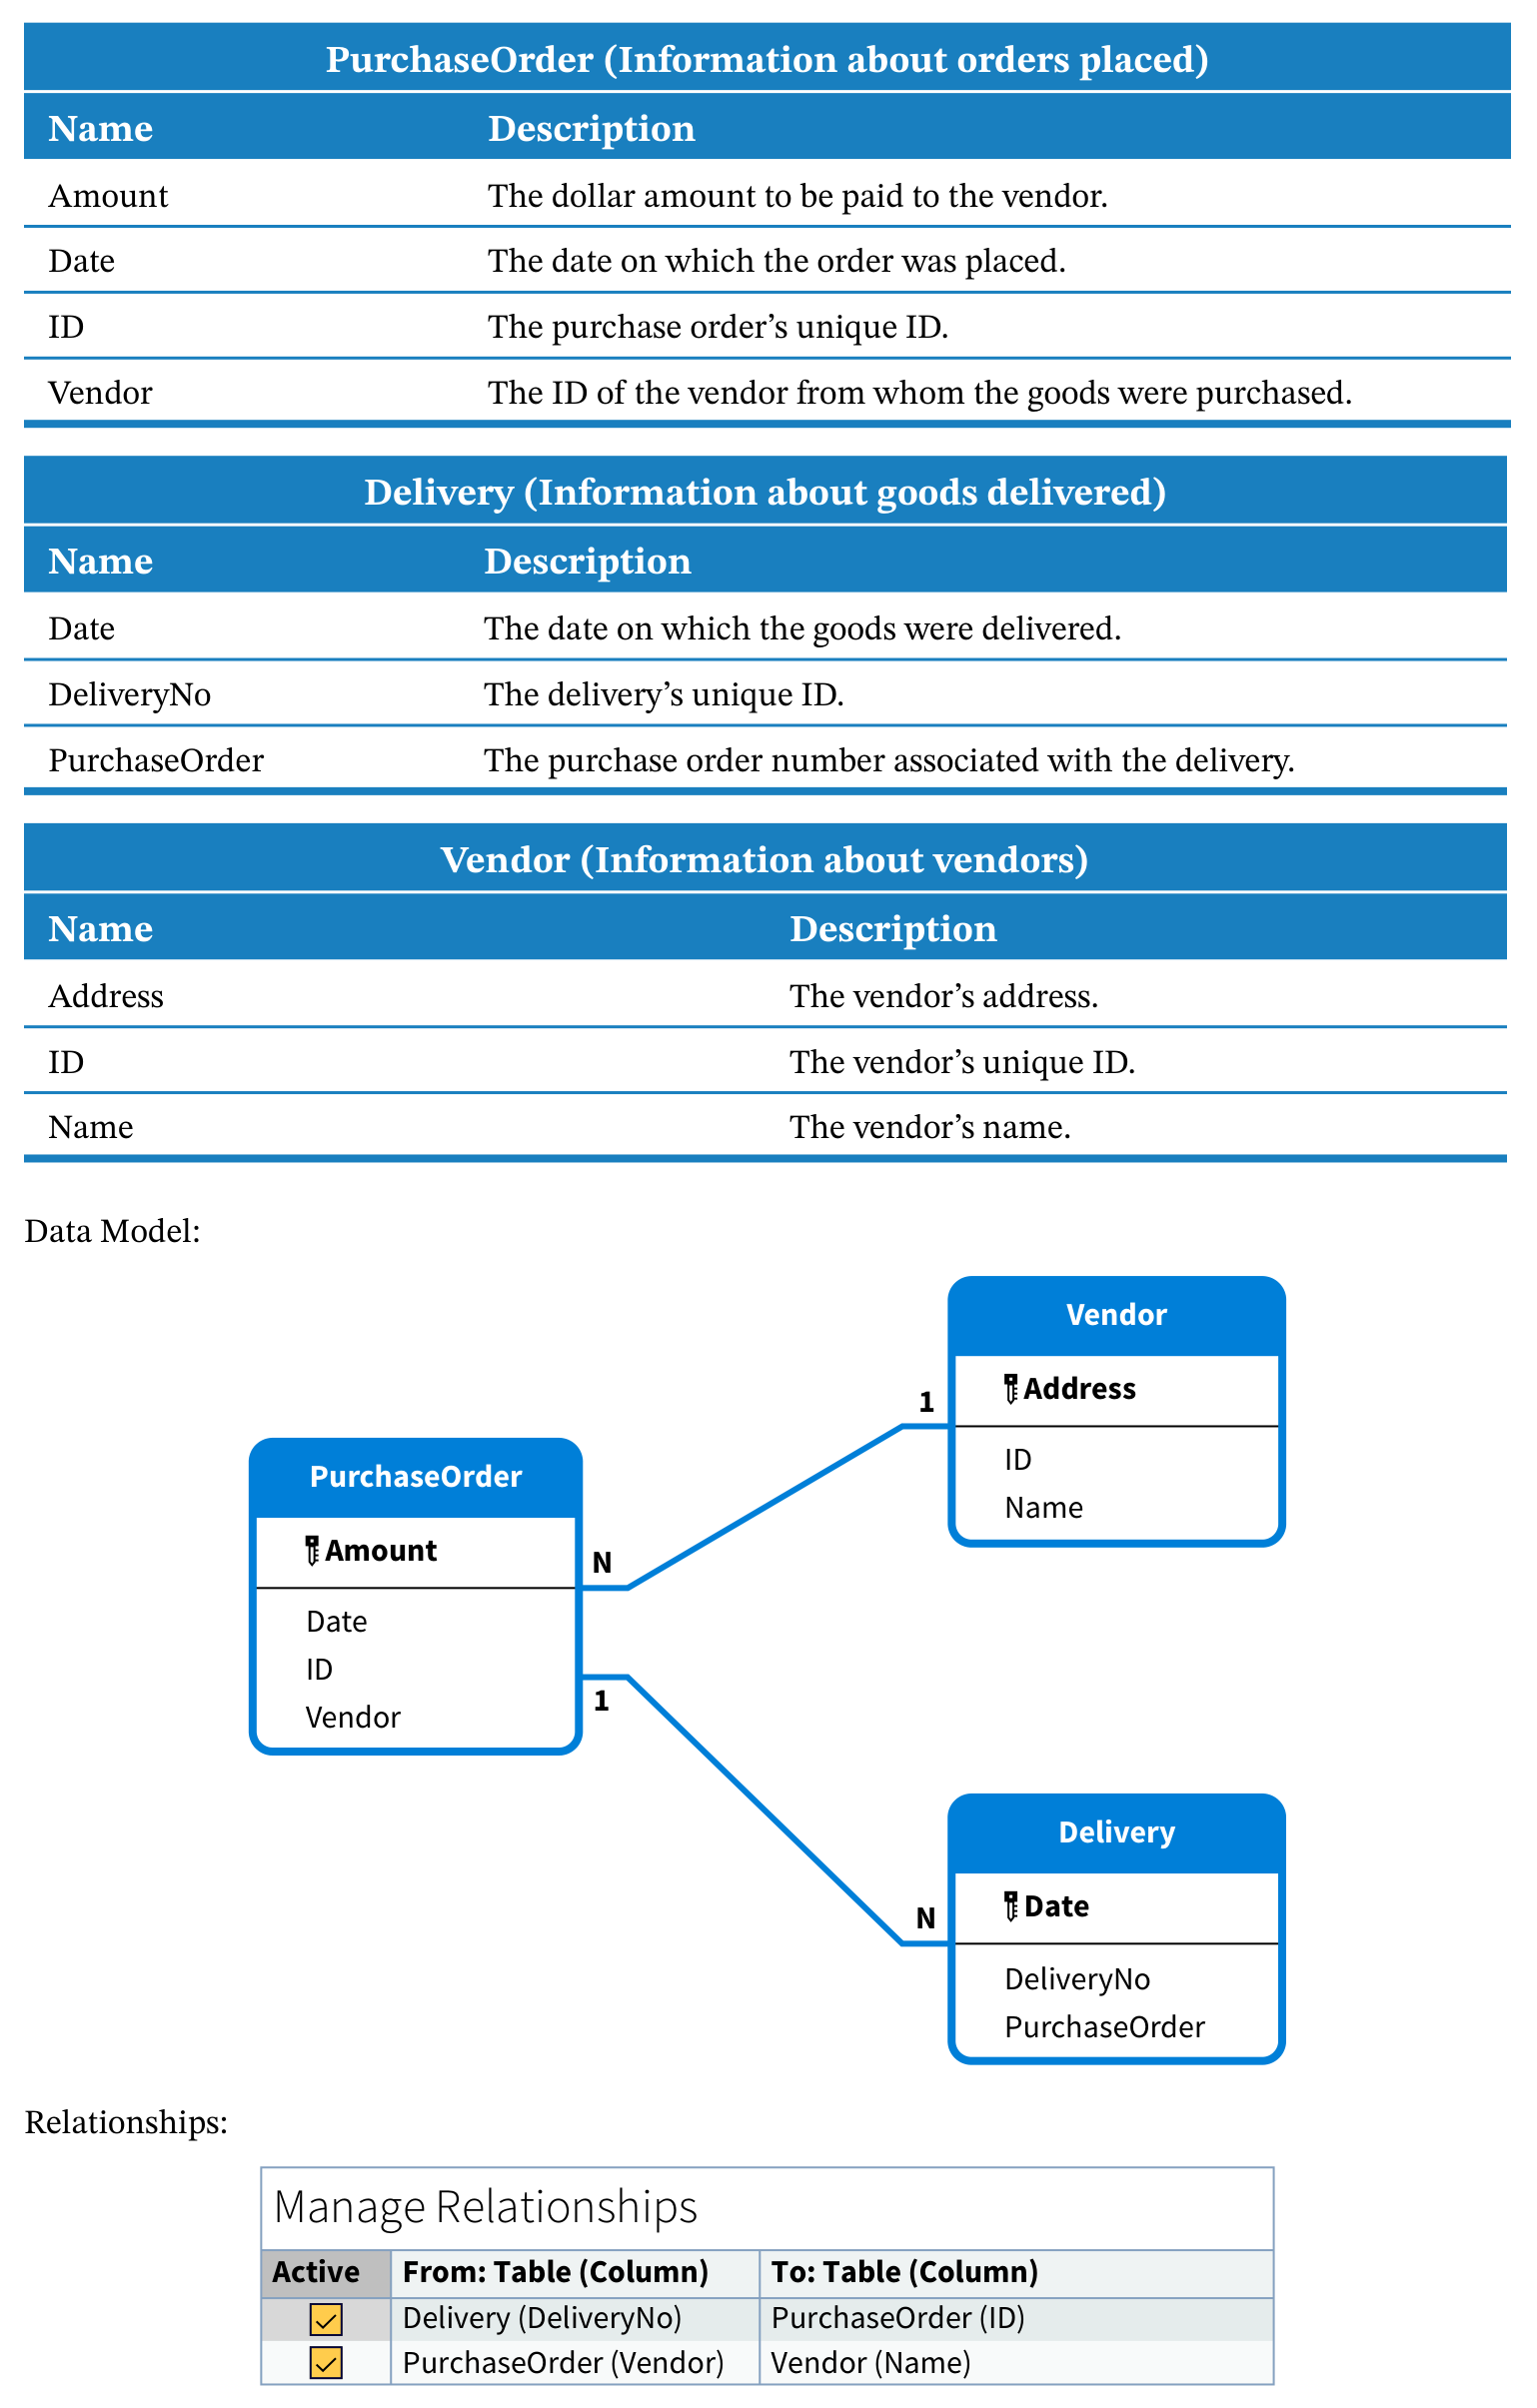
\includegraphics[width=0.95\textwidth,height=0.75\textheight,keepaspectratio]{../textbookForPractice/Figures/Ch_05/BE 5.16.png}
    \end{figure}
\end{frame}

\begin{frame}{Phần Bài tập (Exercises)}
\begin{center}
    \Huge \textbf{Exercises}
\end{center}
\end{frame}

\begin{frame}{EX 5.2 \& EX 5.3}
    \begin{columns}
        \begin{column}{0.5\textwidth}
            \begin{figure}[h]
                \centering
                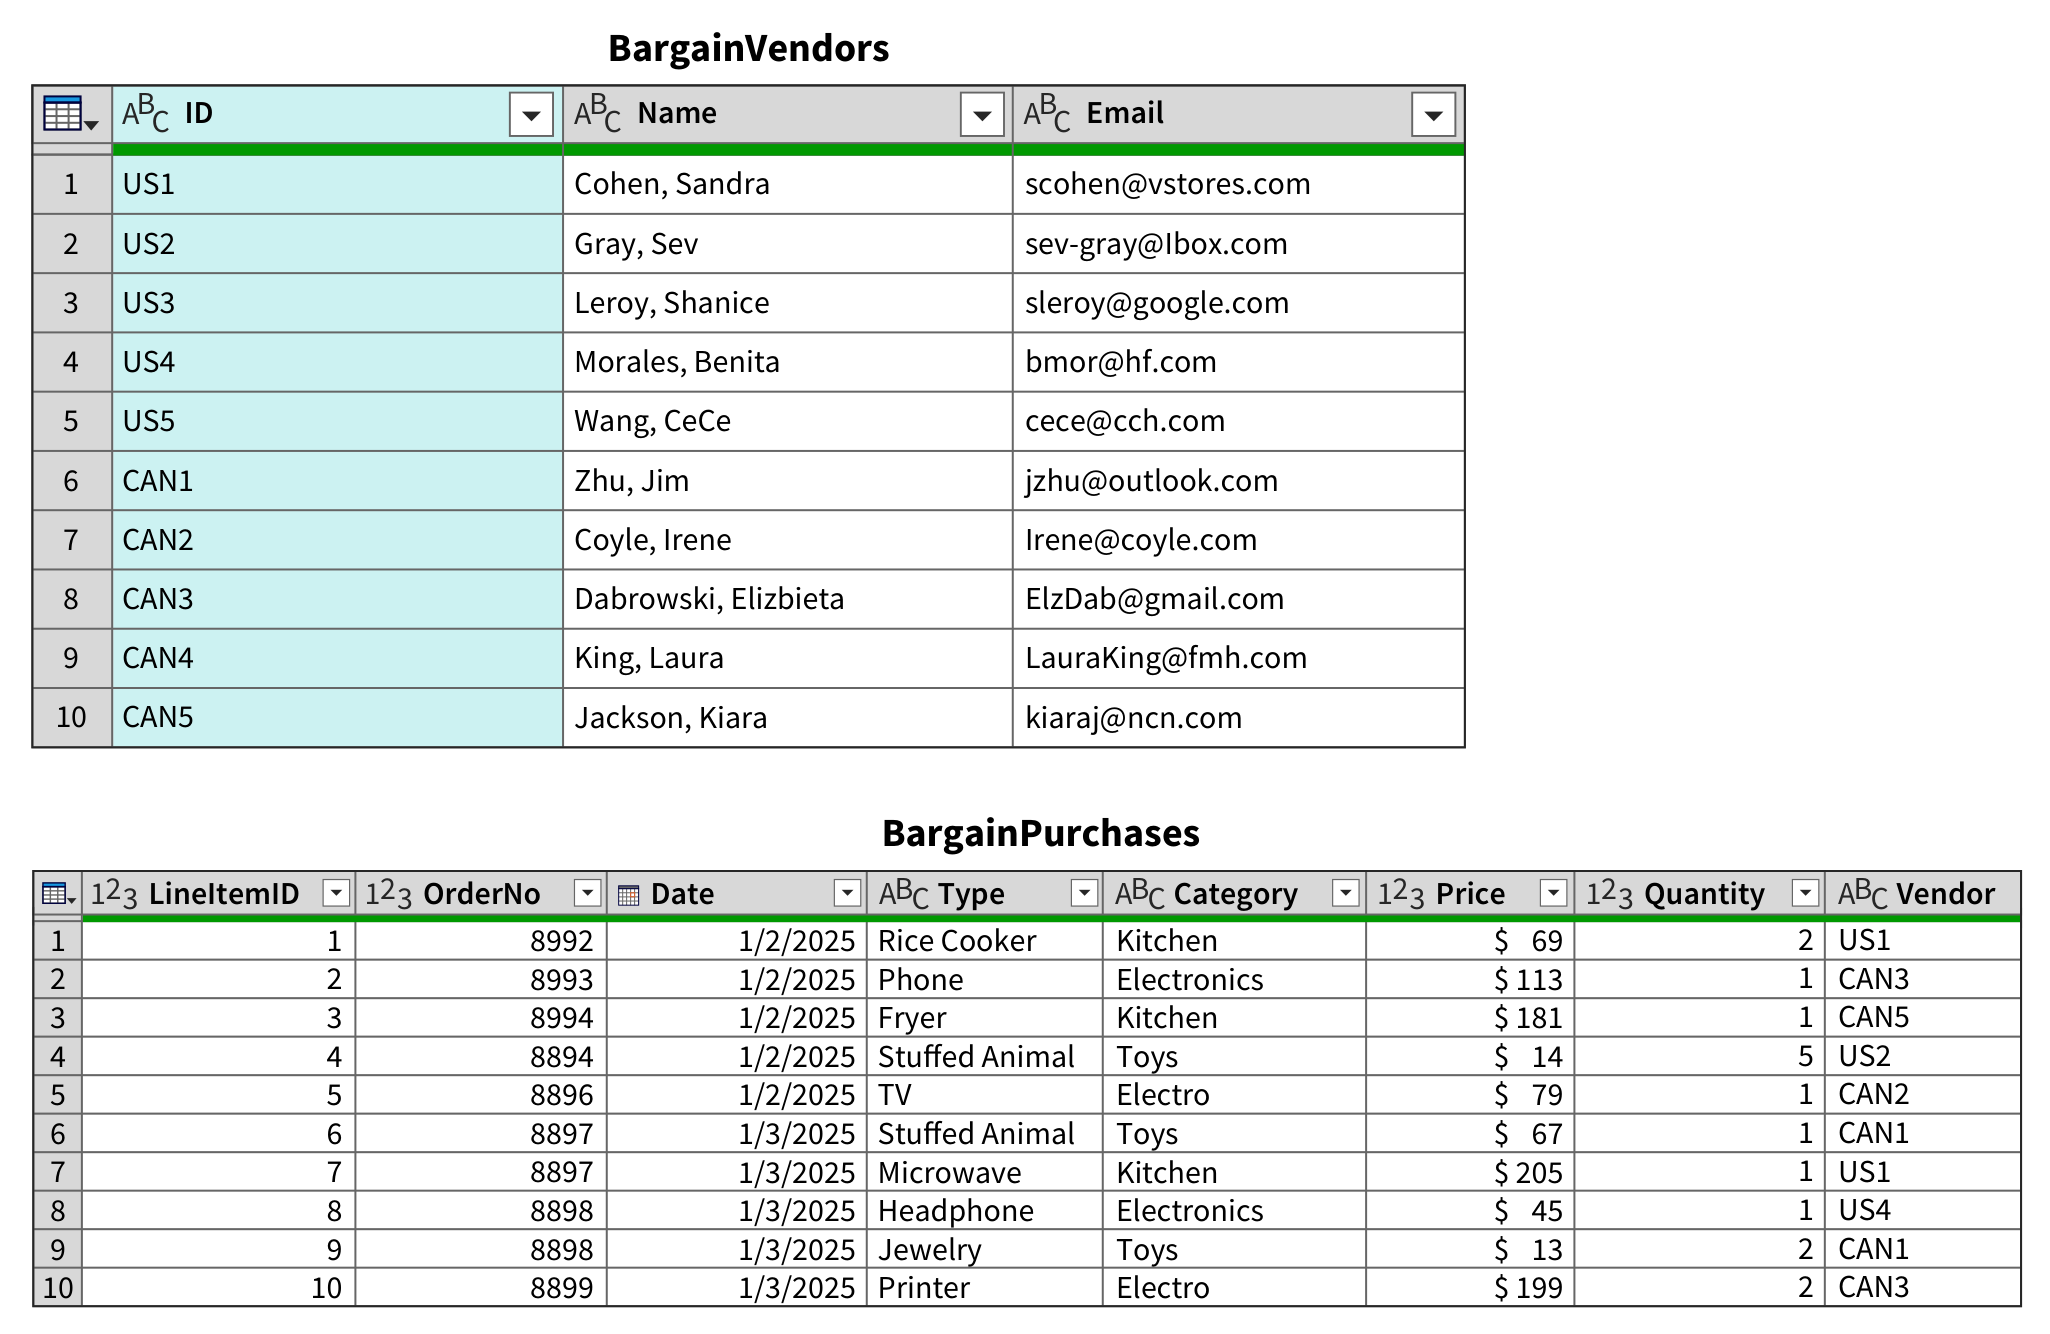
\includegraphics[width=\textwidth,height=0.7\textheight,keepaspectratio]{../textbookForPractice/Figures/Ch_05/EX 5.2.png}
            \end{figure}
        \end{column}
        \begin{column}{0.5\textwidth}
            \begin{figure}[h]
                \centering
                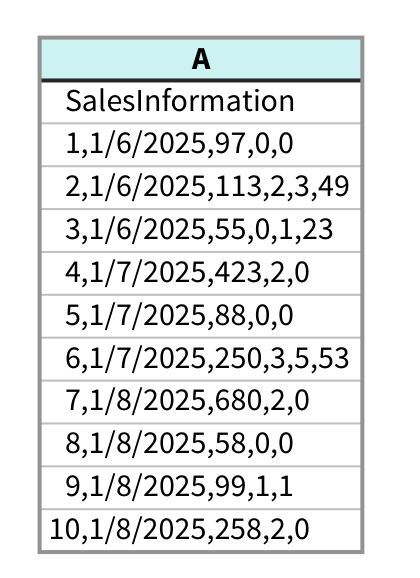
\includegraphics[width=\textwidth,height=0.7\textheight,keepaspectratio]{../textbookForPractice/Figures/Ch_05/EX 5.3.png}
            \end{figure}
        \end{column}
    \end{columns}
\end{frame}

\begin{frame}{EX 5.6 \& EX 5.7}
    \begin{columns}
        \begin{column}{0.5\textwidth}
            \begin{figure}[h]
                \centering
                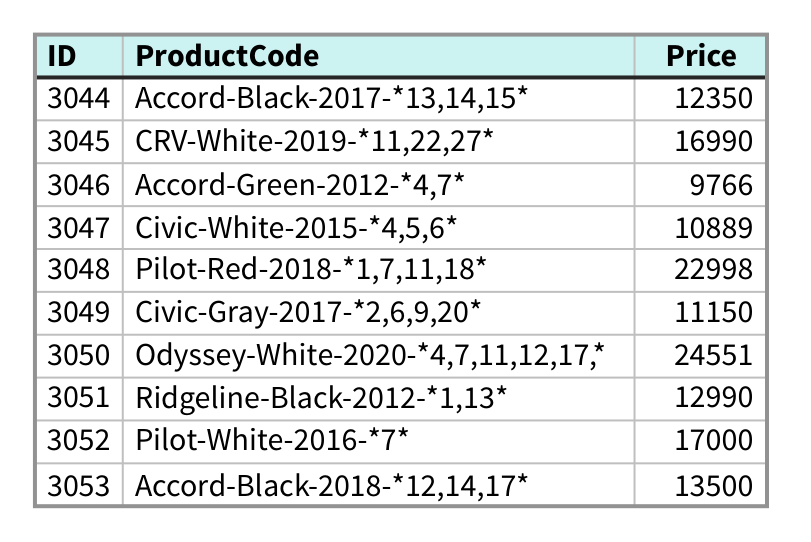
\includegraphics[width=\textwidth,height=0.7\textheight,keepaspectratio]{../textbookForPractice/Figures/Ch_05/EX 5.6.png}
            \end{figure}
        \end{column}
        \begin{column}{0.5\textwidth}
            \begin{figure}[h]
                \centering
                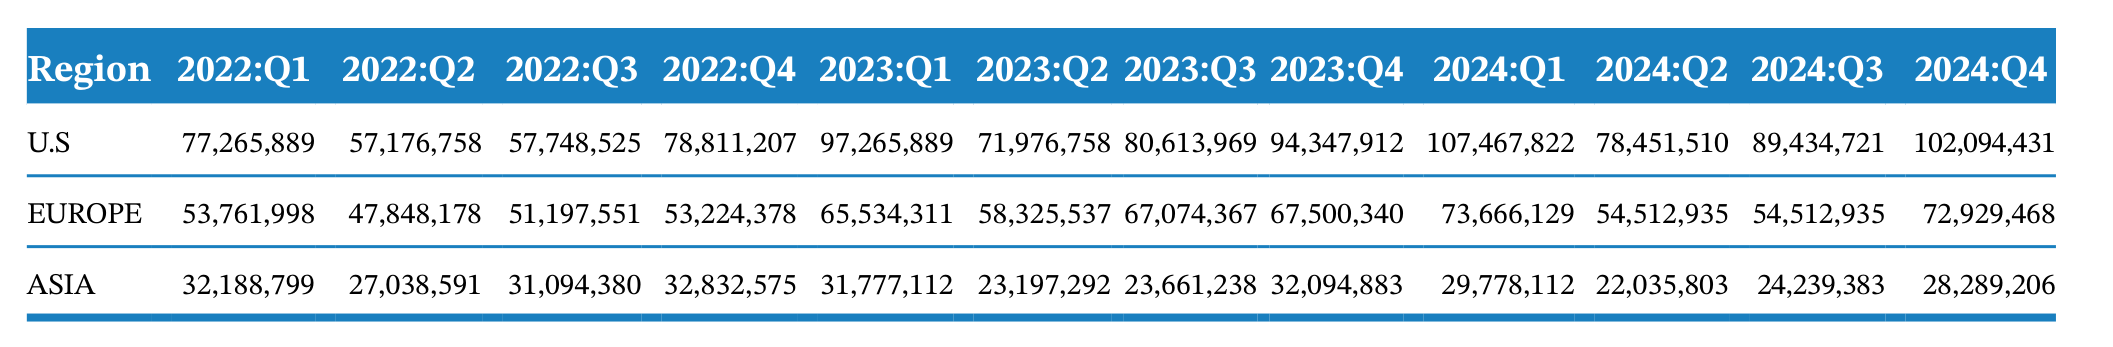
\includegraphics[width=\textwidth,height=0.7\textheight,keepaspectratio]{../textbookForPractice/Figures/Ch_05/EX 5.7.png}
            \end{figure}
        \end{column}
    \end{columns}
\end{frame}

\begin{frame}{EX 5.8}

    \begin{figure}[h]
        \centering
        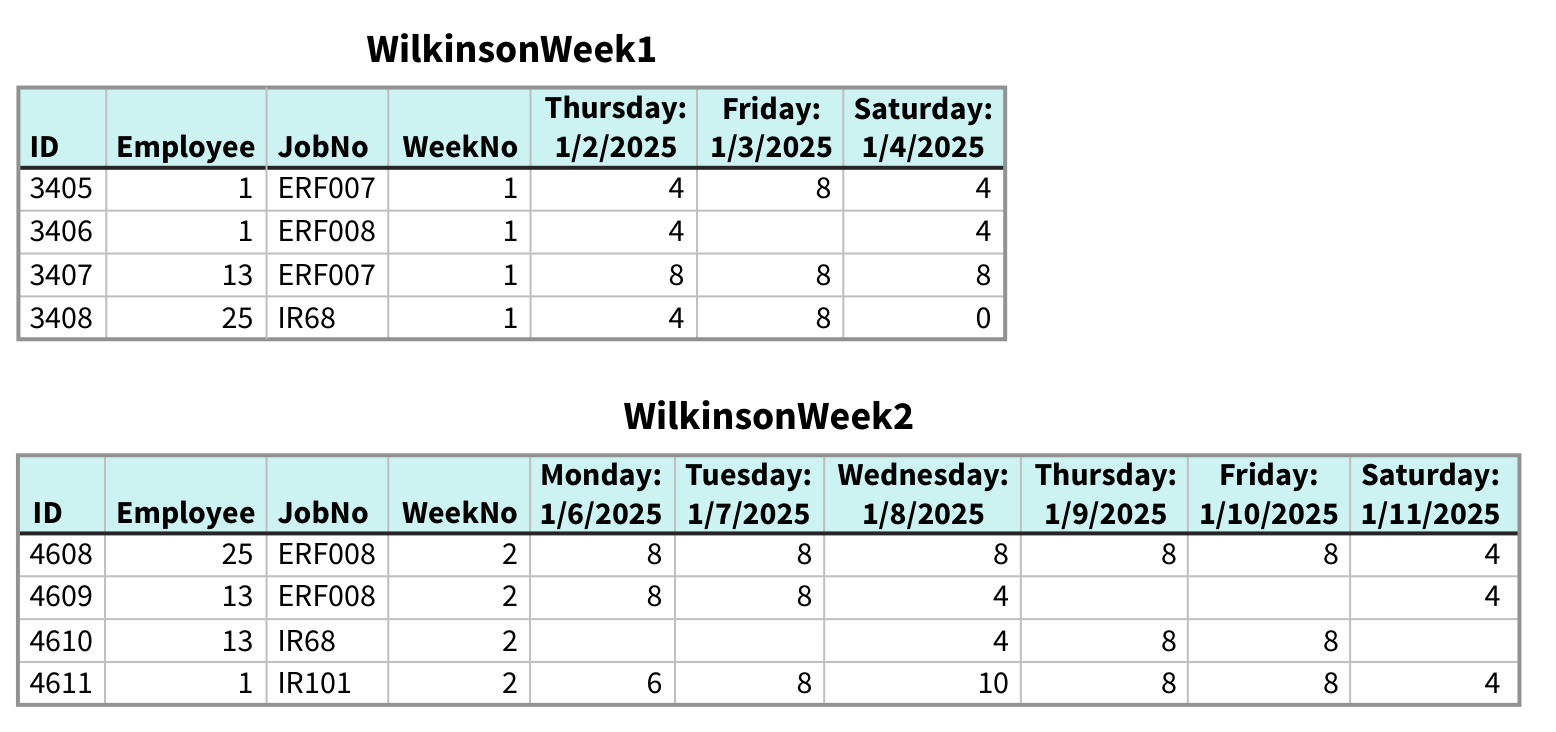
\includegraphics[width=0.95\textwidth,height=0.75\textheight,keepaspectratio]{../textbookForPractice/Figures/Ch_05/EX 5.8.png}
    \end{figure}
\end{frame}

\begin{frame}{Tình Huống Ứng Dụng Chuyên Môn (PAC)}
\begin{center}
    \Huge \textbf{Professional Application Cases (PAC)}
\end{center}
\end{frame}

\begin{frame}{PAC 5.1 \& PAC 5.2}
    \begin{columns}
        \begin{column}{0.5\textwidth}
            \begin{figure}[h]
                \centering
                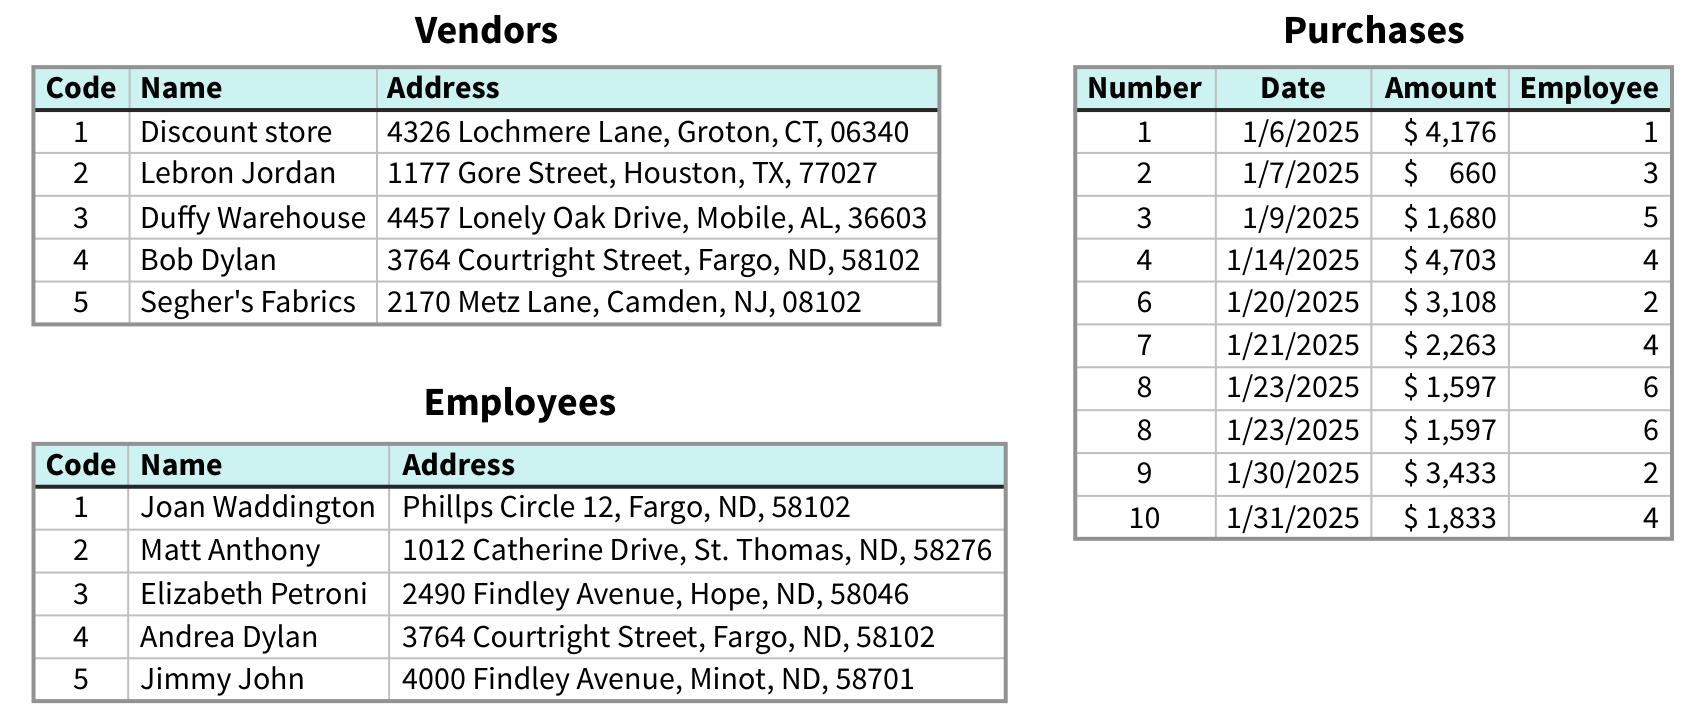
\includegraphics[width=\textwidth,height=0.7\textheight,keepaspectratio]{../textbookForPractice/Figures/Ch_05/PAC 5.1.png}
            \end{figure}
        \end{column}
        \begin{column}{0.5\textwidth}
            \begin{figure}[h]
                \centering
                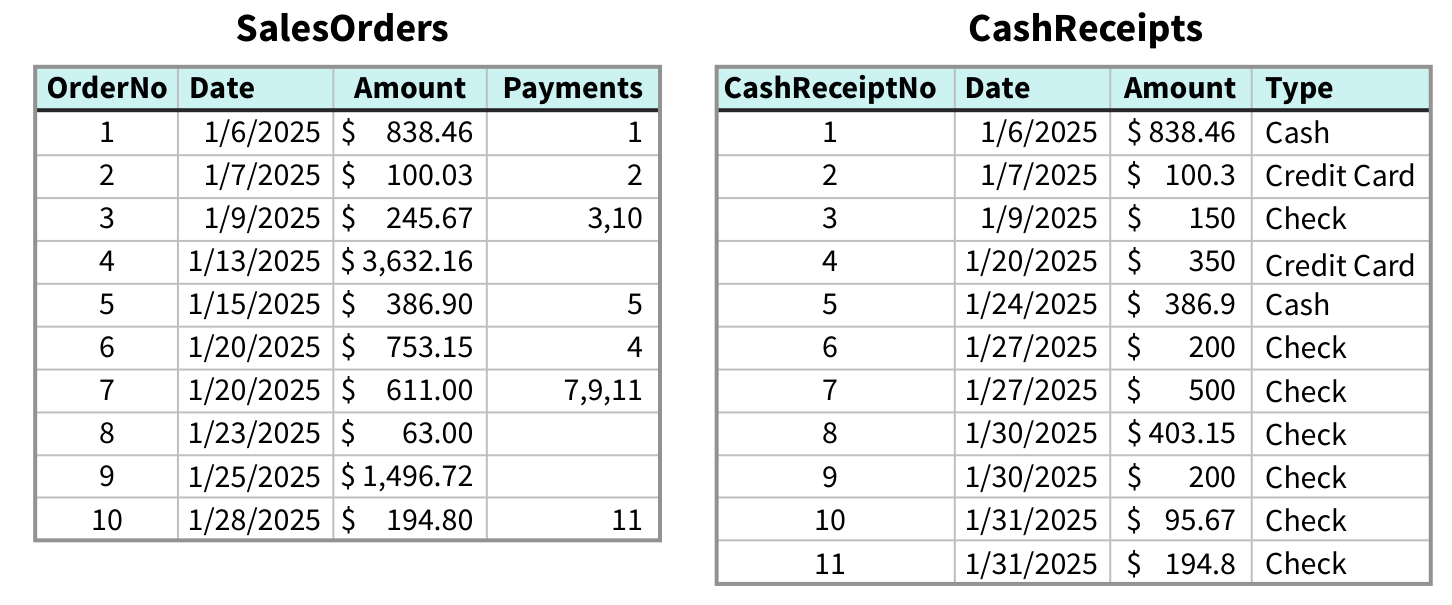
\includegraphics[width=\textwidth,height=0.7\textheight,keepaspectratio]{../textbookForPractice/Figures/Ch_05/PAC 5.2.png}
            \end{figure}
        \end{column}
    \end{columns}
\end{frame}

\begin{frame}{PAC 5.3 \& PAC 5.4A}
    \begin{columns}
        \begin{column}{0.5\textwidth}
            \begin{figure}[h]
                \centering
                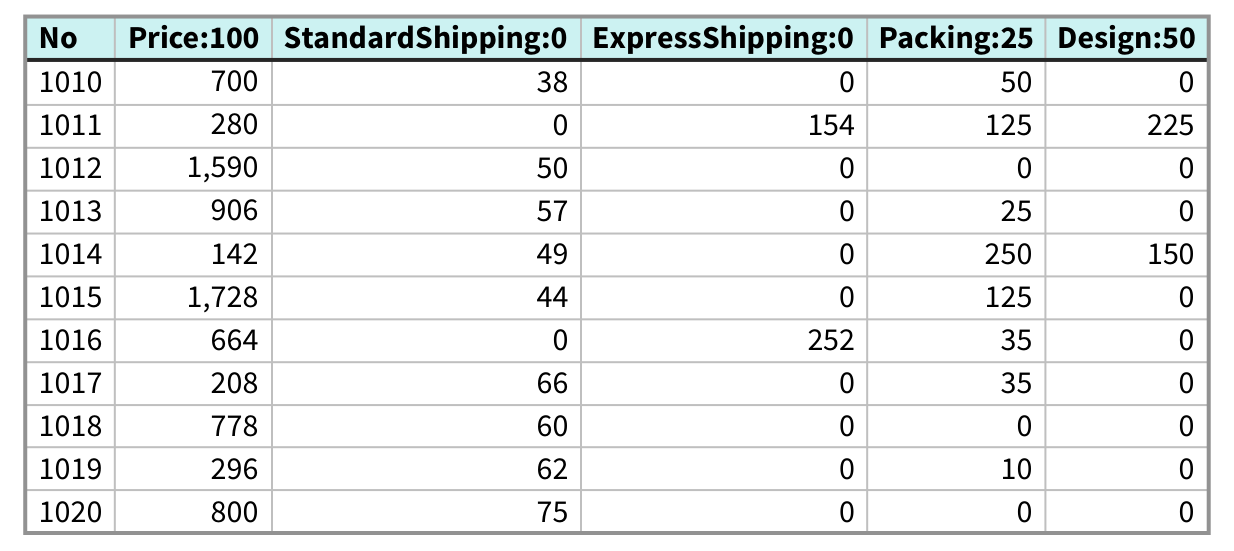
\includegraphics[width=\textwidth,height=0.7\textheight,keepaspectratio]{../textbookForPractice/Figures/Ch_05/PAC 5.3.png}
            \end{figure}
        \end{column}
        \begin{column}{0.5\textwidth}
            \begin{figure}[h]
                \centering
                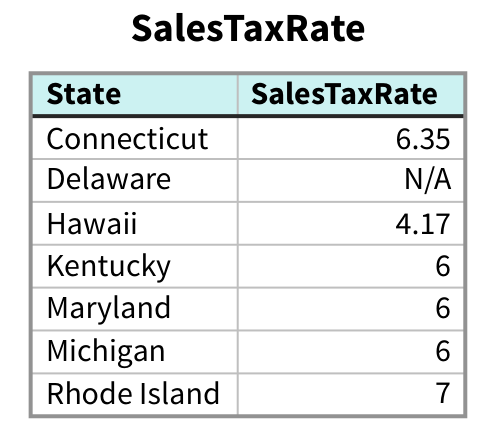
\includegraphics[width=\textwidth,height=0.7\textheight,keepaspectratio]{../textbookForPractice/Figures/Ch_05/PAC 5.4A.png}
            \end{figure}
        \end{column}
    \end{columns}
\end{frame}

\begin{frame}{PAC 5.4B \& PAC 5.4A\_1}
    \begin{columns}
        \begin{column}{0.5\textwidth}
            \begin{figure}[h]
                \centering
                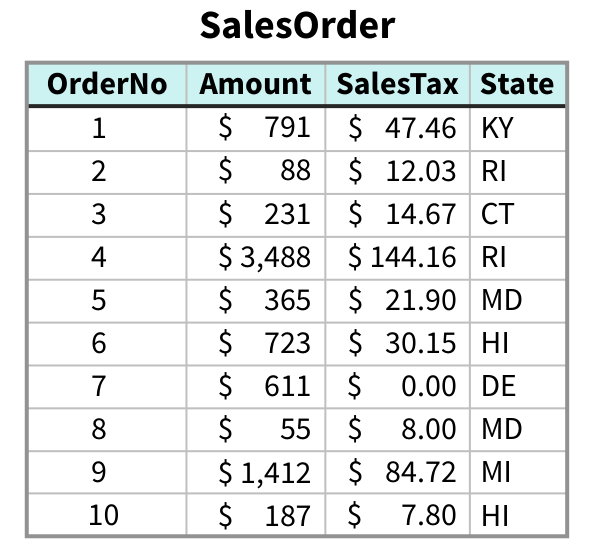
\includegraphics[width=\textwidth,height=0.7\textheight,keepaspectratio]{../textbookForPractice/Figures/Ch_05/PAC 5.4B.png}
            \end{figure}
        \end{column}
        \begin{column}{0.5\textwidth}
            \begin{figure}[h]
                \centering
                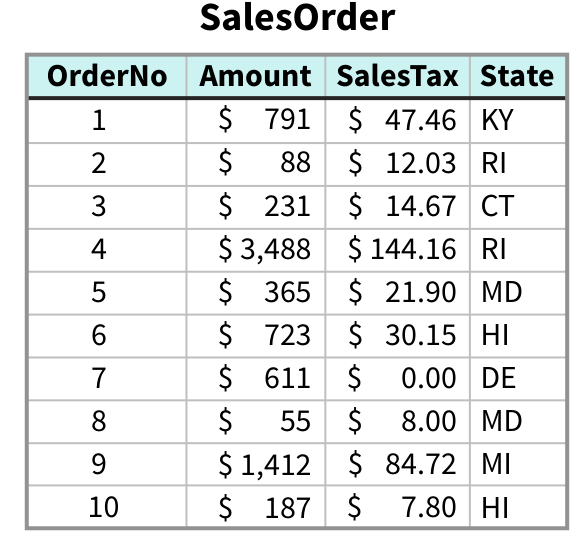
\includegraphics[width=\textwidth,height=0.7\textheight,keepaspectratio]{../textbookForPractice/Figures/Ch_05/PAC 5.4A_1.png}
            \end{figure}
        \end{column}
    \end{columns}
\end{frame}

\begin{frame}{Tóm tắt Mục tiêu Học tập Chương 5}
\begin{itemize}
    \item \textbf{LO 5.1:} Data Profiling giúp xác định "sức khỏe" dữ liệu trước khi xử lý.
    \item \textbf{LO 5.2:} Nắm vững vai trò của từng bước trong quá trình ETL.
    \item \textbf{LO 5.3 \& 5.7:} Sử dụng đúng mẫu Trích xuất (Full/Incremental) và mẫu Tải (Refresh/Incremental) để tối ưu hiệu suất.
    \item \textbf{LO 5.4 - 5.6:} Áp dụng thành thạo các kỹ thuật chuyển đổi Cột (Clean, Split), Bảng (Join, Append), và xây dựng Mô hình dữ liệu chuẩn (Star Schema).
\end{itemize}
\end{frame}

\begin{frame}{Applying critical thinking 5.3}
    \begin{figure}[h]
        \centering
        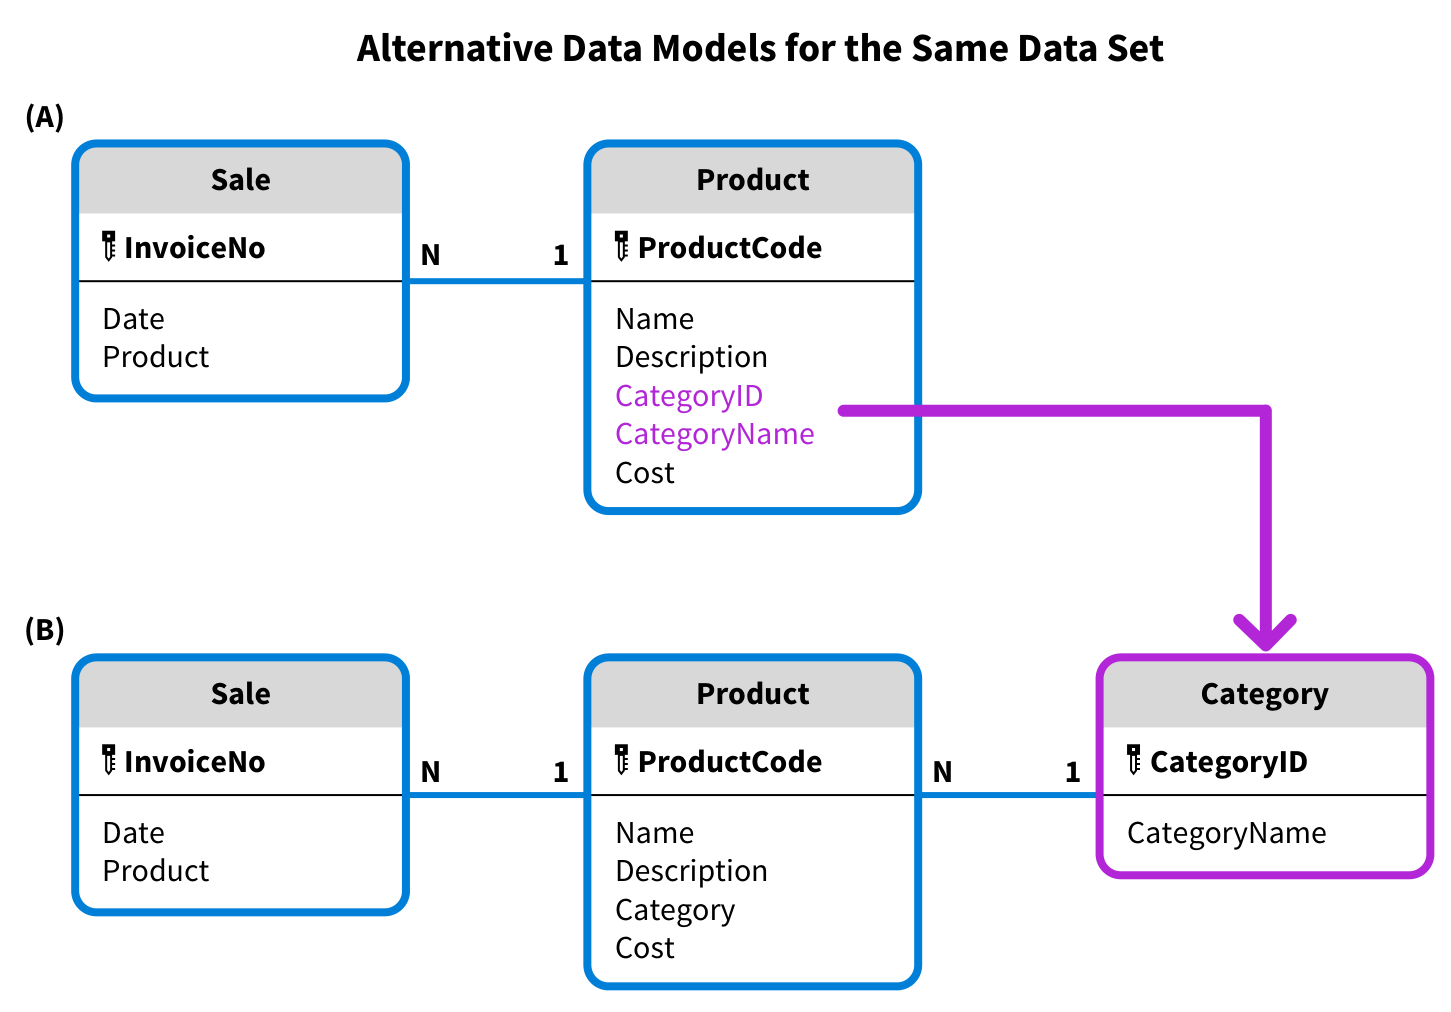
\includegraphics[width=0.95\textwidth,height=0.75\textheight,keepaspectratio]{../textbookForPractice/Figures/Ch_05/Applying critical thinking 5.3.png}
    \end{figure}
\end{frame}

\begin{frame}{LO 6.0}
    \begin{figure}[h]
        \centering
        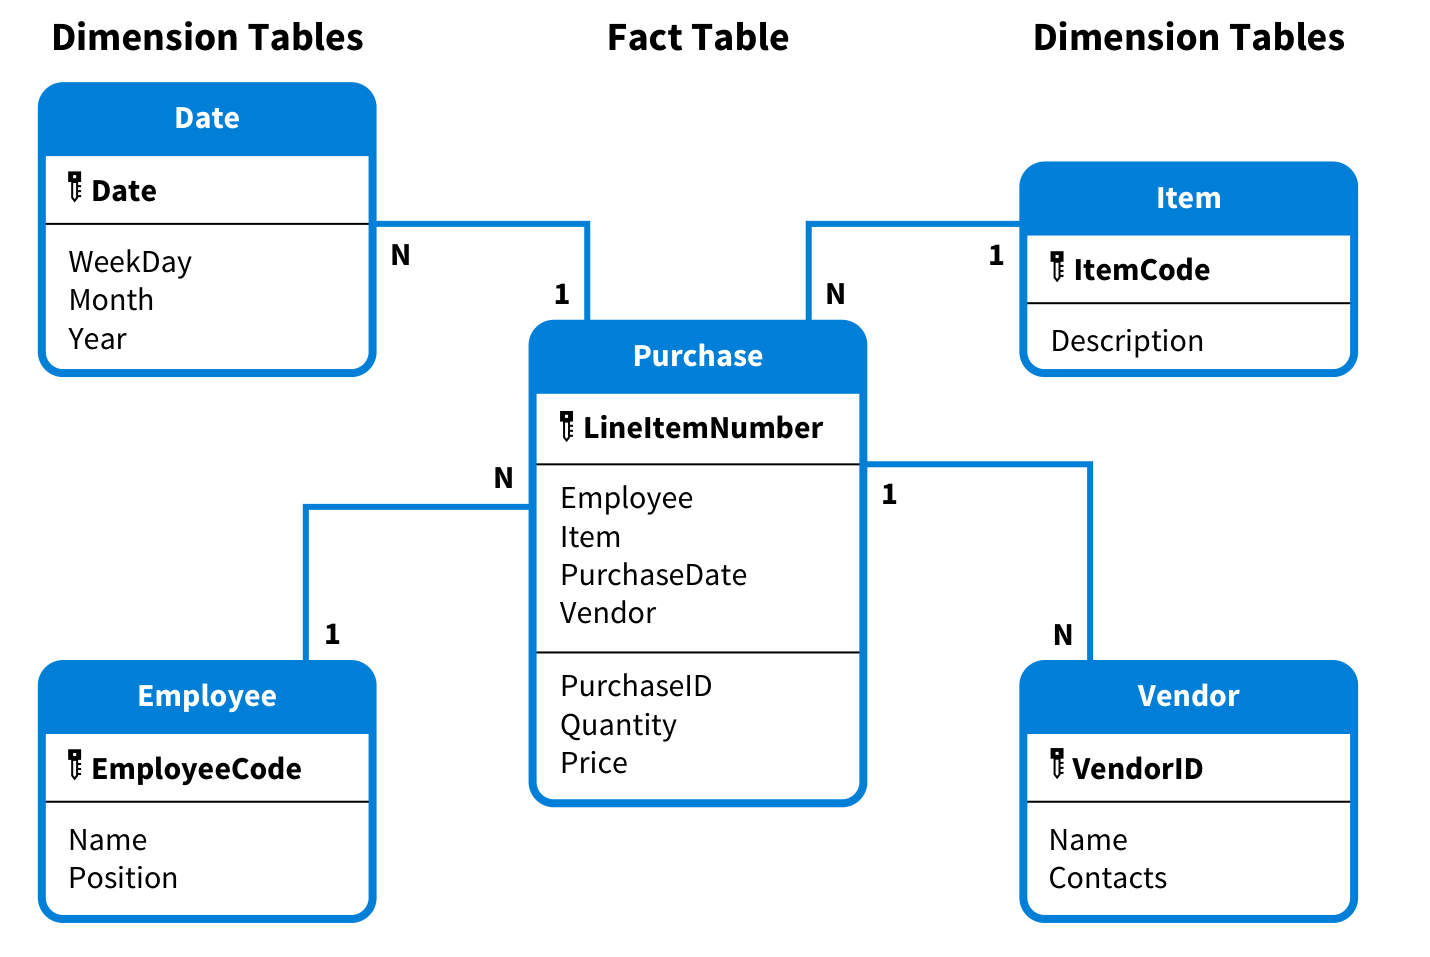
\includegraphics[width=0.95\textwidth,height=0.75\textheight,keepaspectratio]{../textbookForPractice/Figures/Ch_05/LO 6.0.png}
    \end{figure}
\end{frame}

\begin{frame}{LO 7.0}
    \begin{figure}[h]
        \centering
        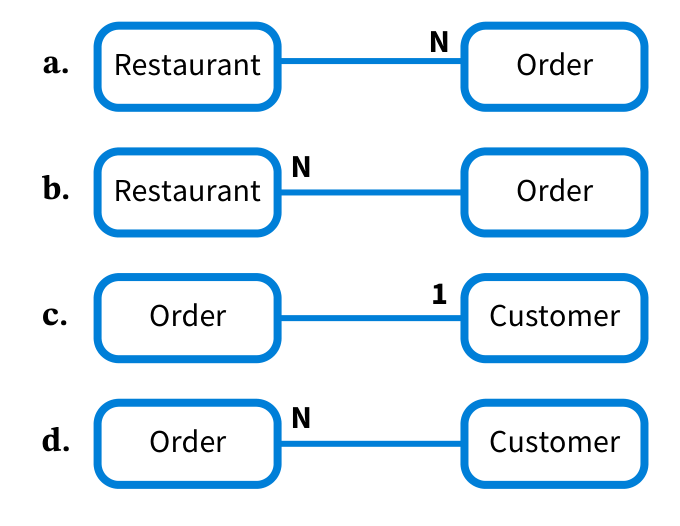
\includegraphics[width=0.95\textwidth,height=0.75\textheight,keepaspectratio]{../textbookForPractice/Figures/Ch_05/LO 7.0.png}
    \end{figure}
\end{frame}

\begin{frame}{Kết thúc}
    \begin{center}
        \Huge \textbf{Hỏi \& Đáp} \\
        \vspace{1cm}
        \Large Cảm ơn các bạn đã lắng nghe!
    \end{center}
\end{frame}

\end{document}
